%==================================================================================================
%   LUKES THESIS TEMPLATE 1.2
%   -------------------------
%   This template is based upon the offcial IMM PhD Thesis template, it is enhanced with a number
%   of new features and a number of errors have fixed. This template is intended to be complied to
%   PDF using PDFLATEX and is tested using the MiKTeX 2.9 LaTeX distribution.
%   It is based on the official DTU-IMM Thesis template by Finn Kuno Christensen in 2009.
%   Small bugfixes by Kasper Laursen in 2012.
%   -------------------------
%   Last Updated: 2012-09-19
%   Contact: lthhe@imm.dtu.dk
%
%	Edited by Emilio Potenza & Marco Galardini
%==================================================================================================
%
%==================================================================================================
% DOCUMENT SETUP
%==================================================================================================
\documentclass[11pt,twoside]{book}                  %Official DTU-IMM Thesis document setup
%
%Set to 'print' for printed version, use 'net' for online version
\def\thesisversion{print}
%
%==================================================================================================
% PACKAGES
%==================================================================================================
\usepackage{LukeThesis}                             %Import Thesis base style
%input{PhDMacros}
\usepackage[width=15pt, height=50pt]{thumbs}							   %Macros for thumb-index

\newcommand{\newthumb}{\addthumb{Section \thechapter}{\thechapter}{black}{gray}}
\newcommand{\myparagraph}[1]{\paragraph{#1}\mbox{}\vspace{10pt}\\}                                   %Thesis specific macros

%
%==================================================================================================
% MANUAL EMILIO, GALA & GIOVANNI :)
%==================================================================================================
\usepackage{mathptmx}
\usepackage{svg}
\usepackage{textcomp}
\usepackage{lscape}
%\usepackage{se­qs­plit}
%\usepackage{gensymb}
\linespread{1.15}


%
%==================================================================================================
% THESIS PROPERTIES (Modifiy these fields with your details)
%==================================================================================================
\def\thesisauthor{Giovanni Bacci}                     %Author
\def\thesistitle{}  %Title
\def\thesishandin{31 December}                       %Submission date (Day-Month}
\def\thesisdegree{PhD}                              %Degree ('B.Eng', 'B.Sc.', 'M.Sc.' or 'PhD')
\def\thesisyear{2014}                               %Submission year
\def\thesisnumber{1}                             %DTU-IMM Serial number (do not include year
\def\thesisISSN{1}                          %ISSN number

\def\thesiskeywords{}  %PDF keywords
\derivethesisprops                                  %Derive dependent properties

\setlength\parindent{0pt}   % no indent in all text
%
%==================================================================================================
% SECTION NUMBERING SETUP
%==================================================================================================
\setcounter{tocdepth}{3}                            %2 adds sections up to subsections
\setcounter{secnumdepth}{3}                         %Subsubsections get a number when this is 3
%
%==================================================================================================
% THESIS STRUCTURE  (Modifiy to include more chapters etc)
%==================================================================================================
\begin{document}
%------------------------
%Pre-frontmatter material
%------------------------
\coverfrontmatter
\preprefrontmatter
%\fancyprefrontmatter
\prefrontmatter

\normalsize
%--------------------
%Frontmatter material
%--------------------
\frontmatter
\pagenumbering{roman}                               %Set frontmatter numbering style


%*******************************************************
% Acknowledgments
%*******************************************************
\pdfbookmark[1]{Quotes}{quotes}

\thispagestyle{empty}

\begin{flushright}{\slshape
	\textit{The secrets of evolution are time, and death: there's an unbroken thread that stretches between those first cells and us} \\
	Carl Sagan \\*[0.5cm]
	\textit{A man provided with paper, pencil, and rubber, and subject to strict discipline, is in effect a universal machine} \\
	Alan Turing \\*[0.5cm]
	\textit{All history is one immortal man who continually learns} \\
	Pascal, cited by Philip K. Dick \\*[0.5cm]
	\textit{In the most carefully constructed experiment under the most carefully controlled conditions, the organism will do whatever it damn well pleases}\\
	Chip Morningstar \& F. Randall Farmer}
\end{flushright}



\newpage

\begingroup
\let\clearpage\relax
\let\cleardoublepage\relax
\let\cleardoublepage\relax

\chapter{Acknowledgements}

First of all I would like to thank my supervisors: Professor \textbf{Alessio Mengoni} and Doctor \textbf{Anna Benedetti} for their constant presence and contagious enthusiasm.

I also would like to thank the COMBO (Florence computational biology group) in the persons of \textbf{Marco Galardini}, \textbf{Marco Fondi} and \textbf{Emanuele Bosi} for their advices and all discussions made over an old whiteboard.

Many thanks to \textbf{Francesco Vitali} for sharing with me the experience of a PhD in the Department of Biology of the Florence University.

Thanks to all of those who have gravitated around the Specola and Sesto Fiorentino during these years, and especially \textbf{Alice Checcucci}, \textbf{Isabel Maida}, \textbf{Elena Perrin}, \textbf{Angela Frascella}, \textbf{Giulia Spini} and \textbf{Amaranta Focardi} for all the good laughs.

Many thanks to my family which has always supported me in all these long years of neverending studies: I wouldn't have made it without their presence.

Last but not least, thanks to \textbf{Adele Giannetti} for standing by me every time I was not-so-enthusiastic about what was going on.

\endgroup



                            %Acknowledgements
\markboth{}{}                                       %Set headings (left)(right)

%*******************************************************
% Publications
%*******************************************************
\pdfbookmark[2]{Publications}{publications}

\chapter{Publications list}

Most of the data presented in this thesis has been published in the following \textit{peer-reviewed} papers:
\begin{itemize}

\item \textbf{Bacci, G.}, Bazzicalupo, M., Benedetti, A., \& Mengoni, A. (2014). StreamingTrim 1.0: a Java software for dynamic trimming of 16S rRNA sequence data from metagenetic studies. \textit{Molecular ecology resources}, 14(2), 426-434.

\item Mengoni, A., Focardi, A., \textbf{Bacci, G.}, \& Ugolini, A. (2013). High genetic diversity and variability of bacterial communities associated with the sandhopper \textit{Talitrus saltator} (Montagu)(Crustacea, Amphipoda). \textit{Estuarine, Coastal and Shelf Science}, 131, 75-82.

\item \textbf{Bacci, G.}, Pagoto, E., Passaponti, M., Vannocci, P., Ugolini, A., \& Mengoni, A. (2014). Composition of supralittoral sediments bacterial communities in a Mediterranean island. \textit{Annals of Microbiology}, 1-13.

\item Borruso, L., \textbf{Bacci, G.}, Mengoni, A., De Philippis, R., \& Brusetti, L. (2014). Rhizosphere effect and salinity competing to shape microbial communities in \textit{Phragmites australis} (Cav.) Trin. ex-Steud. \textit{FEMS microbiology letters}, 359(2), 193-200.

\item Bevivino, A., Paganin, P., \textbf{Bacci, G.}, Florio, A., Pellicer, M. S., Papaleo, M. C., ... \& Dalmastri, C. (2014). Soil Bacterial Community Response to Differences in Agricultural Management along with Seasonal Changes in a Mediterranean Region. \textit{PloS one}, 9(8), e105515.

\item Canfora, L., \textbf{Bacci, G.}, Pinzari, F., Papa, G. L., Dazzi, C., \& Benedetti, A. (2014). Salinity and bacterial diversity: to what extent does the concentration of salt affect the bacterial community in a saline soil?. \textit{PloS one}, 9(9), e106662.

\item \textbf{Bacci, G.}, Bani, A., Bazzicalupo, M., Ceccherini, M.T., Galardini, M., Nannipieri, P., Pietramellara, G., \& Mengoni, A. Evaluation of the performances of Ribosomal Database Project (RDP) Classifier for taxonomic assignment of 16S rRNA metabarcoding sequences generated from Illumina-Solexa NGS. Manuscripts in press in \textit{Journal of Genomics}.

\end{itemize}

% Book chapter
\noindent \textit{Book chapter}
\begin{itemize}

\item \textbf{Bacci, G.} (2015). Raw Sequence Data and Quality Control. In \textit{Bacterial Pangenomics} (pp. 137-149). Springer New York.

\end{itemize}


% Submitted for publication
\noindent \textit{Submitted for publication}

\begin{itemize}

\item \textbf{Bacci, G.}, Ceccherini, M.T., Bani, A., Bazzicalupo, M., Castaldini, M., Galardini, M., Giovannetti, L., Mocali, S., Pastorelli, R., Pantani, O.L., Arfaioli, P., Pietramellara, G., Viti, C., Nannipieri, P., \& Mengoni, A. Exploring the dynamics of bacterial community composition in soil: the pan-bacteriome approach. Manuscripts submitted to: \textit{Antonie van Leeuwenhoek}.

\item \textbf{Bacci, G.}, Abdelrhman, K.F.A., Marras, B., Nistri, A., Schintu, M., Ugolini, A., \& Mengoni, A. The gut microbiota of talitrid amphipods provides insight into the ecology of supralittoral sediments detritivors. Manuscripts submitted to: \textit{FEMS Microbiology Ecology}.

\item Paganin, P., Fiscarelli, E.V., Tuccio, V., Chiancianesi, M., \textbf{Bacci, G.}, Morelli, P., Dolce, D., Dalmastri, C., De Alessandri, A., Lucidi, V., Taccetti, G., Mengoni, A., \& Bevivino, A. Changes in Cystic Fibrosis Airway Microbial Community Associated
with a Severe Decline in Lung Function. Manuscripts submitted to: \textit{PloS one}.

\item Galardini, M., Spini, G., Rossi, M., Roncaglia, B., Bani, A., \textbf{Bacci, G.}, Pini, F., Brilli, M., Biondi, E.G., Bazzicalupo, M., \& Mengoni, A. Evolution of intra-specific regulatory networks in \textit{Sinorhizobium meliloti}. Manuscripts submitted to: \textit{PLOS Computational Biology}

\end{itemize}


% Other articles in preparation related to this thesis
\textit{In preparation}

\begin{itemize}

%\item Di Carli M., De Rossi P., Paganin P., Del Fiore A., Lecce F., Capodicasa C., Bianco L., Perrotta G., Mengoni A., \textbf{Bacci, G.}, Benvenuto E., Vitali F., Daroda L., Dalmastri C., Donini M., Bevivino A. Bacterial community composition and proteome content of fresh-cut lettuce as affected by packaging.

\item \textbf{Bacci, G.}, Paganin, P., Lopez, L., Vanni, C., Dalmastri, C., Cantale, C., Daddiego, L., Perrotta, G., Taccetti, G., De Alessandri, A., Fiscarelli, E.E., Lucidi, V., Bevivino, A., \& Mengoni, A. Taxonomic signatures of CF airway microbiota distinguish between stable and severe declining patients. Manuscripts to be  submitted to: \textit{Proceedings of the National Academy of Sciences}


\end{itemize}


% Conference papers
\textit{Conference papers}

\begin{itemize}

\item \textbf{Bacci, G.} (2012, June). \textit{Elementi di Bioinformatica}. Paper presented at Scuola di Biodiversità e Bioindicazione della Società Italiana Scienza del Suolo. Rome, Italy.

\item \textbf{Bacci, G.}, Bazzicalupo, M., Benedetti, A., \& Mengoni, A. (2013, October). \textit{StreamingTrim 1.0: a Java software for dynamic trimming of 16S rRNA sequence data from metagenetic studies}. Paper presented at Bioinformatiha 2. Florence, Italy.

\item \textbf{Bacci, G.}, Bazzicalupo, M., Benedetti, A., \& Mengoni, A. (2013, December). \textit{StreamingTrim 1.0: a Java software for dynamic trimming of 16S rRNA sequence data from metagenetic studies}. Poster presented at 2\textsuperscript{nd} T\"{u}nen symposium on soil Metagenomics: mining and learning from metagenomes. Braunschweig, Germany.

\item Canfora, L., \textbf{Bacci, G.}, Pinzari, F., Papa, G. L., Dazzi, C., \& Benedetti, A. (2013, December). \textit{Metagenomic approach applied to the microbial community of a saline soil with high spatial variability}. Poster presented at 2\textsuperscript{nd} T\"{u}nen symposium on soil Metagenomics: mining and learning from metagenomes. Braunschweig, Germany.

\item \textbf{Bacci, G.} (2014, May). \textit{Inspecting the dynamics of bacterial communities. The pan-bacteriome approach}. Paper presented at Cortona Procarioti. Cortona, Italy.

\item \textbf{Bacci, G.}, Bazzicalupo, M., Benedetti, A., \& Mengoni, A. (2014, May). \textit{StreamingTrim 1.0: a Java software for dynamic trimming of 16S rRNA sequence data from metagenetic studies}. Paper presented at PhD Day\textsuperscript{5}. Sesto Fiorentino, Italy.

\end{itemize}

%The source files of this thesis will be available after the discussion as a git repository on \href{https://github.com/mgalardini/PhDGala}{GitHub} (@mgalardini).
									%Publication list
\markboth{}{}

%*******************************************************
% Abstract
%*******************************************************
\pdfbookmark[3]{Abstract}{abstract}
\chapter{Abstract}
Bacteria are everywhere and they make up for their microscopic dimension in sheer number. Thanks to their great functional and taxonomic variability, bacteria plays a pivotal role in several environments. In soil they are responsible for some of the most important biogeochemical cycles and for the cycling of organic compounds. They reside even on both the surface and in deep layers of human skin, in the saliva and oral mucosa, in the conjunctiva, and in the gastrointestinal tracts performing tasks that can be useful for the human host. They were able to colonize extreme environments and, thanks to their ability to break down hazardous substances into less toxic or non toxic substances, they are used as bioremediation agents for removing pollutant from contaminated sites. Nevertheless, the study of microbial diversity patterns is still hampered by the enormous diversity of microbial communities and the lack of resources to sample them exhaustively.\\
Difficulties in bacterial cultivation and isolation are even today one of the main obstacle for the correct identification of both bacterial taxonomies and bacterial functions. A range of novel methods, most of which are based on rRNA and rDNA analyses, have uncovered part of the microbial diversity in several environments but the percentage of characterized organisms remains low (approximately 1-5\% of the whole bacterial biodiversity). The next step in the ``genomic era'' is to extract genomic, taxonomic and functional informations directly from bacterial communities genome (the metagenome). This concept moved our perspective of bacterial diversity to a ``meta'' point of view. To this end, the advent of the Next Generation Sequencing (NGS) techniques has made it technically possible to exhaustively sequence entire bacterial communities without the need to isolate single strains. Therefore, developing new methods and protocols for studying bacterial patterns in different environments is becoming one of the most competitive challenge to date.\\
The work here presented is part of this perspective and it can be easily divided into three different major parts. The first one (named ``Small tools for big data") deals with all issues related to processing and exploitation of sequence data in a metagenomic analysis. In particular, performing this kind of analysis require generating a huge amount of data which can't be easily managed even by most sophisticated computers. For this reason is crucial developing bioinformatic algorithms able to handle a big number of sequences with a small amount of memory and processor resources. Results obtained within this part of the work have underlined the need both to improve available tools and to develop new software for analysing metagenomic data. Specifically, one of the most used tool for taxonomic classification of rRNA sequences from metabarcoding analyses was benchmarked: the ``Ribosomal Database Project'' Classifier (RDP Classifier). This analysis has shown a decreasing level of resolution passing from Phylum to Genus level highlighting the need of continuous improvements in current classification algorithms. On the other hand, a new tool for quality refinement of metagenomic data has been developed. This tool is able to remove low quality segments from raw sequence data retaining as much information as possible. Furthermore, the amount of memory required for this tool to work is proportional to the length of the sequence analysed and it is not related to the number of sequences to analyse, making this tool very useful for metagenomics analyses.\\
The second part of this work includes three different chapters named: ``Bacteria-environment interaction'', ``A life in transition: bacteria in harsh environments'' and ``Bacteria in agro-environments''. Basically, this part covers both functional and taxonomic classification of bacteria in different environments. In particular, changes in bacterial community composition have been inspected from three different perspectives: natural environments, extreme environments and agricultural environments. In all these ambiances, bacteria were found capable of shaping their composition based on either external perturbing agents (anthropic gradient, salinity, pollution...) or time. Developing methods for studying bacterial community is one of the crucial tasks in metagenomics where even obtain an overview of bacterial community data could be a very difficult task (especially in complex environment like soil).\\
In the last part of my work, bacterial communities have been analysed as both human and animal hosts. From the animal side, the gut microbiota of talitrid amphipods has been analysed in order to inspect changes in bacterial communities related to different species and locations. Results obtained have shown that is possible to generate a bacterial fingerprint for both inspected factors, underlining that, either different species or different diets are able to influence bacterial gut composition. From the human side, the composition of bacterial communities has been inspected in patients with a specific pathological conditions: cystic fibrosis. Understanding differences in bacterial populations related to this pathological state is very important for either developing new treatments or improving existing ones. In addition, reported results highlight the importance of microbiome inspection for the selection of bacterial groups that may be related to the uprising of a particular human disease.\\                                   %English summary of Thesis
\markboth{}{}                                       %Set headings (left)(right)

%*******************************************************
% Sommario
%*******************************************************
\pdfbookmark[4]{Sommario}{sommario}
\chapter{Sommario}
\begin{otherlanguage}{italian}

I batteri sono capaci di colonizzare quasi tutti gli ambienti presenti sul pianeta terra. Infatti, grazie alla loro plasticità funzionale e tassonomica, sono in grado di giocare un roulo importante in molti ambienti diversi. Nel suolo sono tra i principali responsabili del ciclo dei compositi organici ed altri importanti cicli biogeochimici ma riescono a vivere anche all'interno di organismi più grandi come ad esempio l'uomo. Infatti intere comunità batteriche sono state caratterizzare in diversi distretti del corpo umano come: sulla pelle, nella saliva, nella mucosa orale, ma anche nella congiuntiva e nel tratto gastrointestinale svolgendo funzioni essenziali per lo sviluppo dell'ospite. La loro plasticità li rende in grado di crescere e colonizzare anche gli ambienti più estremi e, grazie alla loro capacità di trasformare sostanze pericolose in sostanze poco (o per niente) tossiche, sono utilizzati anche come agenti per la bioremediation. Purtroppo però lo studio delle popolazioni microbiche rimane difficoltoso sia per la loro grande variabilità che per la mancanza di metodi per campionare esaustivamente complesse popolazioni.\\
Uno dei maggiori ostacoli all'identificazione di specie batteriche è la coltivazione e l'isolamento delle specie di interesse in condizioni di laboratorio. Infatti è stimato che solo l'1\% dei batteri sia in grado di essere coltivato e studiato usando metodi microbioloigici standard. Metodi di analisi innovativi, la maggiorn parte dei quali basati sull'analisi della sequenza del DNA ribosomiale, hanno permesso di scoprire nuove specie e funzioni batteriche ma la percentuale dei microorganismi caratterizzati rimane bassa (circa 1-5\% della biodiversità batterca totale). Il prossimo passo nell'era genomica sarà l'estrazione delle informazioni tassonomiche e funzionali direttamente dal genoma delle comunità batteriche (il cosiddetto ``metagenoma''). Questa sfida sta spostando la concezione della diversità batterica verso una prospettiva ``meta''. Per questo l'avvento delle tecniche di sequenziamento di nuova generazione (NGS) ha reso tecnicamente possibile il sequenziamento di intere comunità batteriche senza il bisogno di isolare singole specie. Lo sviluppo di nuovi metodi e protocolli per lo studio dei pattern batterici in ambienti diversi sta diventando una delle sfide più difficili dei nostri tempi.\\

\end{otherlanguage}                                   %Italian summary of Thesis
\markboth{}{}                                       %Set headings (left)(right)


%------------------
% Table of contents
%------------------

\newpage\mbox{}\newpage
\chaptermark{Contents}
\pdfbookmark{\contentsname}{toc}
\renewcommand{\sectionmark}[1]{\markright{#1}}
\sectionmark{Contents}
\addtolength{\parskip}{-\baselineskip}
\tableofcontents
\addtolength{\parskip}{\baselineskip}
\renewcommand{\sectionmark}[1]{\markright{\thesection\ #1}}

%------------------
% List of figures
%------------------

\newpage\mbox{}\newpage
\chaptermark{Figures list}
\pdfbookmark{Figures list}{toc}
\renewcommand{\sectionmark}[1]{\markright{#1}}
\sectionmark{Figures list}
\addtolength{\parskip}{-\baselineskip}
\listoffigures
\addtolength{\parskip}{\baselineskip}
\renewcommand{\sectionmark}[1]{\markright{\thesection\ #1}}

%------------------
% List of figures
%------------------

\newpage\mbox{}\newpage
\chaptermark{Tables list}
\pdfbookmark{Tables list}{toc}
\renewcommand{\sectionmark}[1]{\markright{#1}}
\sectionmark{Tables list}
\addtolength{\parskip}{-\baselineskip}
\listoftables
\addtolength{\parskip}{\baselineskip}
\renewcommand{\sectionmark}[1]{\markright{\thesection\ #1}}

%-------------
% Main content
%-------------

\mainmatter
\part{Introduction}
\newthumb
%%%%%%%%%%%%%%%%%%%%%%%%%%%%%%%%%%%%%%%%%%%%%%
\logvartrue
\chapter{Background}
%%%%%%%%%%%%%%%%%%%%%%%%%%%%%%%%%%%%%%%%%%%%%%

Bacteria are often cited as examples of one of the Earth's most primitive living forms. Unfortunately, they are still associated almost exclusively to infection diseases. The reality is rather different, in fact only a very small fraction of bacteria is able to cause infections in contrast to a highly diversified and beneficial bacterial world. Most of them not only reciprocally support each other but their immensely varied and efficient metabolism also defines and sustains balanced environments (the biosphere). Solidarity among bacterial cells is one of their most important characteristic. Even infection-causing bacteria are able to benefit from this solidarity, making them more resilient and ``inventive'' than isolated species. In the last 20 years, the development of genomic tools have revolutionized microbial ecological studies and strongly expanded our view on this previously under appreciated microbial world. It is encouraging to see that evolution and ecology are now emerging as regular subjects within microbiology. The next decade should be one of gradually changing and enlarging perspective regarding the place of bacteriology in the biological sciences. There are now comforting signs that we are moving towards a deeper and more realistic appreciation of the roles played by bacteria on our planet.

\section{The Bacterial world}
Microorganisms are essentially everywhere in nature and they have been integral to the history and function of life on Earth. However, until very recently, their importance has been appreciated by only a few specialist. Indeed, bacteria are still most often considered from an anthropocentric point of view, focusing our attention only on the relatively few pathological species and the potential of microorganisms to provide us with useful products and services (\textbf{da mettere un paio di references}). This is a very constrained perspective if we think that bacteria have been the sole form of life on Earth for some two billion years, playing central roles in climatic, geological, geochemical, and biological evolution \cite{cavalier2006cell}.\\
The bacterial world contains a highly heterogeneous group of organisms sharing only one common characteristic, their small size. The patterns of bacteria distribution are influenced by environmental factors such as temperature, pH, salinity, pressure, the presence of nutrients and the sources of carbon and energy \citep{gerhard1986bacterial}. These factors are able to shape Earth's bacterial communities distribution in respect to both space and time, influencing the selective proliferation of a set of bacteria in a distinct environment, based on their metabolic characteristics. Bacteria can use many different types of metabolic strategies and bacterial species can often be differentiated from each other based on their metabolic characteristics. The specific metabolic properties of a microbe are one of the major factors in determining that microbe’s ecological niche, and they can be used to classify bacteria in different metabolic groups (Figure~\ref{fig:bacmet}). Thanks to their high variability, bacteria have been, and still are able to colonize almost every ecological niche in nature.\\
\begin{figure}[!tb]
	\centering
	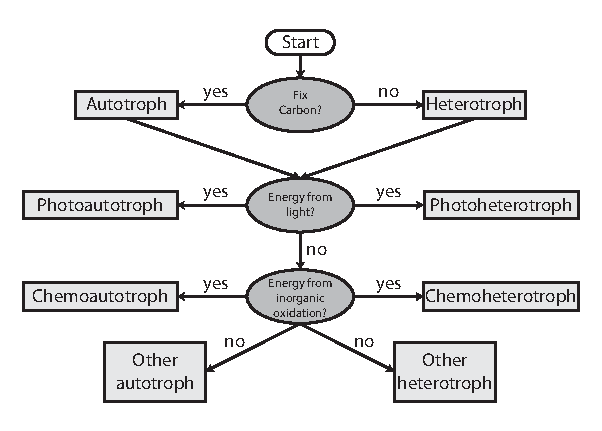
\includegraphics[width=0.7\textwidth]{./figures/Introduction/bacterial_metabolism_bw}
  	\caption{General flowchart used for metabolic classification of bacteria. \label{fig:bacmet}}
\end{figure}
Giving their ability to thrive in a vast set of different environments, bacteria play pivotal roles in several biogeochemical cycles and are responsible for the cycling of organic compounds. They have been found in all kind of environments ranging from the human gut \cite{walter2011human}, to the rhizosphere \cite{philippot2013going}, to conventionally inhospitable habitats such as acid mine run-off \cite{simmons2008population} and geothermal hot springs 	\cite{sharp2014humboldt}. Studies based on cultured microbes have revealed that they are critical components of these environments providing them with essential services \cite{van2008unseen, arrigo2004marine}. For example, the Earth's cycles of hydrogen, carbon, nitrogen, oxygen and sulphur are driven largely by microbial catalysed redox reactions (Figure \ref{}). These reactions require multimeric protein complexes evolved exclusively in microorganism such as bacteria \cite{falkowski2008microbial}. However, a large part of these processes is still unknown making the study of bacterial functions indispensable for the complete comprehension of the dynamics able to modify our planet.\\
Biologists have long appreciated the roles that microbes play in the two distinct disciplines of pathogenesis and ecosystem cycling; although, in these years, the importance of microbes-host association is rapidly growing. Currently, microbes associated with a macroscopic host have their own definition in the word ``microbiota'' coined for the firs time by Joshua Lederberg in 2001 \citep{lederberg2001scientist}. The role of microbiota is occupying a very important position in the host evolution \cite{ley2008evolution}. Indeed, the set of bacteria linked with a macroscopic organism can interact with its host to influence physiology and contribute to health, growth, or fitness \citep{dimkpa2009plant, hooper2012interactions}. For example, studies of model rhizosphere microbiota have taught us that they can impact plant growth \citep{kennedy2007competitive}, stress response \cite{redman2002thermotolerance, yang2009rhizosphere}, and pathogenic defense \cite{cook1995molecular}. In this perspective, for understanding completely a macroscopic organism’s physiology is becoming mandatory the investigation of its microbiota.\\
This great microbial diversity found in various environments (including hosts associated ones) can be measured by a set of indices such as phylogenetic diversity, species diversity, genotype diversity, and gene diversity. Above the species level, microbial diversity has been commonly quantified based on evolutionary distances among observed taxonomic groups from a specific environment. Below this level, microbial diversity has been typically described using population genetic parameters such as gene diversity and genotype diversity. However, despite the fact that species is the fundamental unit of biological classification, what constitute a species remain controversial. In addition, until very recently, most of what we know about microbial diversity and microbial functions were derived from cultured microorganisms . While such studies are essential, the advent of genomic has revolutionized our comprehension of the bacterial world showing that much of what we thought we knew about this microscopic world were in fact highly biased.\\

\subsection{The species concept}
%\begin{wrapfigure}{r}{0.35\textwidth}
%	\vspace{-20pt}
%	\begin{center}
%		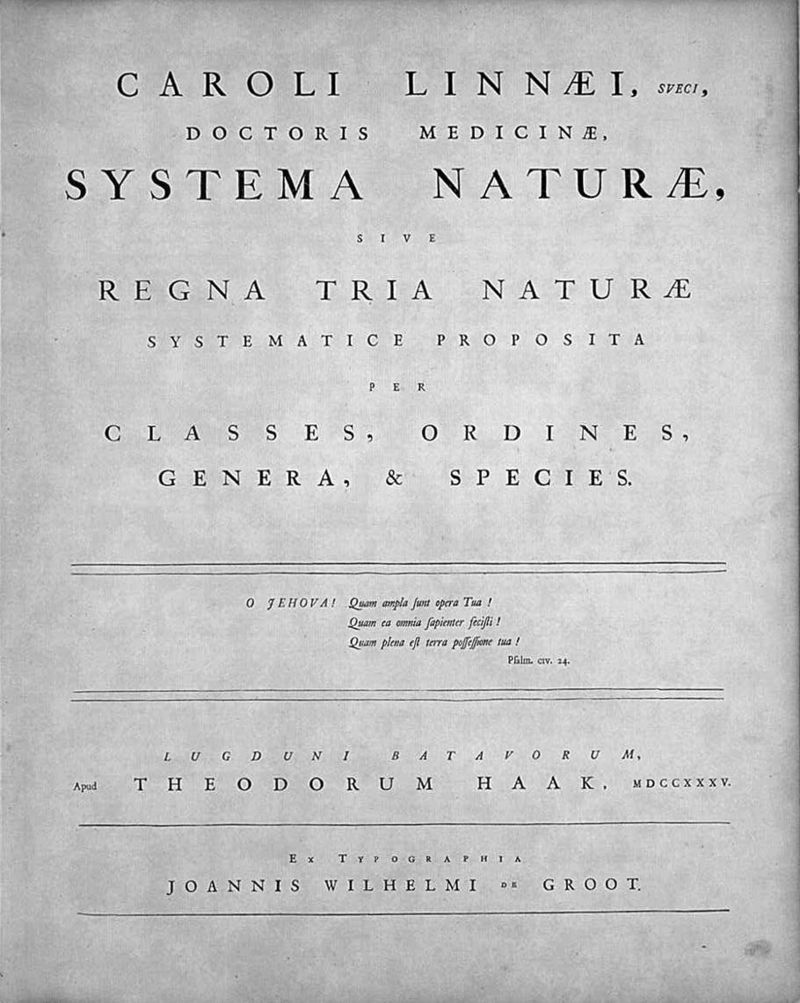
\includegraphics[width=0.33\textwidth]{./figures/Introduction/systema_naturae}
%	\end{center}
%	\caption{The title page of Systema Naturae, Leiden (1735)}
%	\vspace{-10pt}
%\end{wrapfigure}
Attempting to bring order in the astounding variety of organisms with which we share the planet have been an endless human effort. One of the first classification system was developed by Carl Linnaeus in the mid-18th century \cite{linnaeus1800species, bhl10277}. Linnaeus established the existence of three kingdoms: the animal kingdom (\textit{Regnum animale}), the plant kingdom (\textit{Regnum vegetabile}) and the mineral kingdom (\textit{Regnum lapideum}), outlining his ideas for the hierarchical classification of the natural world. In his works Linnaeus did not classify microbes but, since the mid-19th century, his binomial nomenclature has been used by microbiologist to designate microbial species. However, what constitute a species was and remains  controversial especially with the advent of the ``genomic era'' and the explosion of data that it has brought with it \cite{doolittle2006genomics}.\\
Prokaryotic classification is the youngest and most dynamic between all classifications of living organisms. This might be due to the fact that prokaryotes were not even know to exist until a few centuries ago. Developing a prokaryote classification system based on macro-morphological traits, like sexual reproduction or some physical characteristics, has been a very difficult because of their relative simplicity \cite{cowan1965principles}. The absence of useful fossil records, together with the difficulties in identifying possible diagnostic elements from these organisms have concur to the instability of the prokaryote classification system. Indeed, species demarcation in prokaryotes is not defined by a theory-based concept and tends to be more arbitrary, anthropocentric or rooted in practical necessity (e.g. bacteria species like \textit{Neisseria meningitis} or \textit{Bacillus anthracis} have been historically defined on the basis of the disease they cause regardless of other types of considerations).\\
Until the end of the 18th century, no prokaryotic classification was attempted. Ottu M\"{u}ller, a Danish naturalist, was the first to create a systemic arrangement of microorganisms defining two form genera called \textit{Vibrio} and \textit{Monas}; which differentiated the round and elongated type of bacterial cells \cite{logan2009bacterial}. One of the most important step in the classification of microorganisms was the ability to isolate them in pure cultures. Therefore, in 1881, Robert Koch published the first technique of cultivation on a solid media; paving the way for what he called ``the golden age of the medical microbiology''. Following this discovery, researchers were able to retrieve direct informations on a microorganism by cultivating it in pure culture; thus, the amount of bacteria described from the end of the 19th century to the first two decades of the 20th century was impressive. In 1970  a modern identification index for bacteria was first provided with the publication of the ``Bergey's Manual of Determinative Bacteriology''. In the second half of the 20th century the increasing knowledge of the properties DNA, in conjunction with the development of molecular biological techniques pushing the idea that bacteria might be classified using their genomes. Finally, in 1970, the catalogation of the ribosomal RNA (rRNA) and the development of the DNA-DNA hybridization technique permitted to achieve a great breakthrough in the history of bacterial classification \cite{stackebrandt198516, de1975improvements}.\\
Currently, microbial species are defined using the so-called "polyphasic approach", that is grounded on clear rules for both genotypic and phenotypic attributes \cite{vandamme1996polyphasic}. Nowadays, more than 7000 different microbial species have been classified using this approach, but, as actually practised, it faces serious problems. Indeed, the primary criterion for discriminating between different species is a cut-off level for pairwise genomic DNA-DNA hybridization levels; however, this cut-off level has never been based on any particular theoretical assumption \cite{de2005ernst, hey2006failure}. Furthermore, pairwise comparison of microbial strains can be asymmetric (different values can be obtained with the same pair of strains simply exchanging the one used as probe with the one used an target) and intransitive (hybridization levels > 70\% between strains A - B, and A - C may be not necessary the same between B - C). Moreover, a large number of surveys of microbial diversity have equalled species with ``operational taxonomic units'' (OTUs) based on 16S rRNA sequence \cite{ley2006microbial}. However, although 16S rRNA can be used for comparing and classifyning known species, it may have insufficent genetic resolution for the de-novo binning of newly isolated microbes into species. For these reason, newer genomic methods have been developed recently consisting in the identification of discrete sequence clusters based on multiple core genes \cite{fraser2007recombination, gevers2005re}. But all these technical issues are not able to address a primary conceptual question: what is a microbial species?\\
From the beginning of the 20th century the species concept has been redefined multiple times. The first species concept universally accepted was the one developed by Ernst Mayr and then called ``the biological species concept'' (BSC) \cite{mayr1942systematics}. This concept defines species as groups of ``potentially interbreeding natural population which are reproductively isolated from other such groups''. Unfortunately, this definition is not applicable to asexual organisms lacking a meiotic life cycle, as bacteria. In the modern era, other two distinct species concepts have been developed, and both of them are currently accepted by biologist and philosophers. The first one is the ``phenetic species concept'' (PhSC); it is based on ``statistically co-varying characteristics which are not necessarily universal among the members of the taxa'' \cite{claridge1997species, sokal1970biological}. The second one is the ``evolutionary species concept'' (ESC) that defines a species as ``an entity composed of organisms which maintains its identity from other such entities through time and over space, and which has its own independent evolutionary fate and historical tendencies'' \cite{claridge1997species}. However, none of these concepts was specifically developed for the definition of the microbial species; for this reason, several other attempts to fill this gap have been suggested. Here were reported a collection of the most representatives definition of microbial species in order to highlight the lack of consensus:
\begin{itemize}
\item ``A species could be described as a monophyletic and genomically coherent cluster of individual organisms that show a high degree of overall similarity in many independent characteristics, and is diagnosable by a discriminative phenotypic property'' \cite{rossello2001species}.
\item ``Species are considered to be an irreducible cluster of organisms diagnosably different from other such clusters and within which there is a parental pattern of ancestry and descent'' \cite{staley2006bacterial}.
\item ``A species is a group of individuals where the observed lateral gene transfer within the group is much greater than the transfer between groups'' \cite{dykhuizen2005species}.
\end{itemize}
One of the newest concept developed is the so-called method free unitary concept, which defines microbial species as ``metapopulation lineages'' \cite{de2005ernst}. Here, a metapopulation is defined as a set of connected subpopulation and a lineage can be thought of as a metapopulation that extends through time and evolves separately from other lineages. Following this criterion a species does not need to be ``phenotypically distinguible, or diagnosable, or monophiletic, or reproductively isolated, or ecologically divergent, to be species''. The only criterion for a species according to this concept is their evolutionary fate, and no methodological criterion is required for assigning species designations. Although this new conception of microbial species still has not been fully accepted, it continues to have
important consequences. For example its more complete acceptance may provide a solution to the species concept problem, bringing the species concept into line with claims about the general theoretical significance of the species category.\\
Defining the  concept of species for prokaryotes remains a problematic task, despite microbiologists and philosophers have undertaken several efforts to find a correct and shared working scheme. The emergence of new definitions for microbial species is gradually changing the whole concept of prokaryotic evolution in the attempt to find methods and thresholds indipendent criteria. This is giving new life to the study of bacterial genomes as a possible and more comprehensive way for measuring the distance between two different ``metapopulation lineages''.\\

\subsection{Microbial diversity}
Studying natural species in their environment has always been one of the crucial task in Biology and Ecology. For centuries, biologists have studied pattern of plant and animal diversity in different ecological niches; but, until recently, these kind of analyses were impossible for microorganisms even if they were, and still are, one of the most diverse and abundant group of organisms on Earth \cite{curtis2005exploring}. New genetic techniques have revealed extensive microbial diversity that was not possible to to detect with culture-dependent methods. Even though the application of these new techniques, the scientific understanding of microbial distribution patterns is still particularly weak. The definition of new diversity estimators specifically designed for microbial life is needed in order to fully comprehend the role of microorganisms on the planet.\\
In order to inspect the complexity of a natural community the first thing that we ask ourselves is how many different species there are in that community. In other words what we want to know is the ``species diversity'' of the community that we are studying. Species diversity is an abstract measure composed by two component: ``species richness'' ans ``species evenness''. The first component is a measure of the number of different species found; whereas, the latter one quantifies how equal the abundances of these species are \cite{hill1973diversity}. In general species diversity reflects the variety of organisms present in a particular environment; although, speaking about living organisms in an environment requires some considerations. First of all, the community of living organisms able to interact with non-living components of their environment is called an ``ecosystem''. In addition, a single ecosystem can be considered as a composition of multiple smaller habitats that, in turn, are to be considered ecosystems. Giving this great variability how can we refer to the diversity of a single ecological niche or to the whole diversity of an ecosystem?\\
The species diversity of a particular ecosystem is called $\gamma$-diversity and is the sum of two others sub-diversities: the $\alpha$-diversity and the $\beta$-diversity \cite{whittaker1960vegetation}. The term $\alpha$-diversity refers to the mean species diversity in a locale scale like an habitat or a particular site; whereas, the term $\beta$-diversity refers to the differentiation among those habitats or sites (Figure~\ref{fig:diversities}). 
\begin{figure}[!tb]
	\centering
	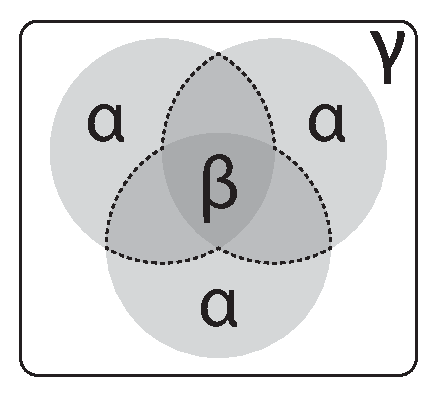
\includegraphics[width=0.7\textwidth]{./figures/Introduction/diversities}
  	\caption{Schematic representation of $\alpha$ (gray circles), $\beta$ (dotted line) and $gamma$ (blach square) diversities.\label{fig:diversities}}
\end{figure}
These indices are linked to the area of interest which can be of different sizes and, the habitats or the sites within it may vary their dimensions, accordingly. Both $\alpha$ and $\gamma$ diversities are subjected to the spatial scale chosen but no consensus has been reached on what spatial scales are appropriate to quantify these indices \cite{whittaker2001scale}. Therefore, it has been proposed that the definition of $\alpha$ and $\gamma$ diversities does not need to refer to a specific spatial scale: these indices can be measured for an existing environment of any size that consists of subunits at any scale. These scale-free definition is not applicable to $\beta$-diversity as it can not be calculated directly from a species data \cite{tuomisto2010diversity}. Beta diversity in his original definition has to be considered as a measure of the species turnover between two sites \cite{whittaker1960vegetation}. The simplest definition of this index is: $\beta = \gamma/\alpha$; where gamma diversity is the total species diversity of a landscape, and alpha diversity is the mean species diversity per habitat. Here $\beta$-diversity quantifies how many subunits there would be if the total species diversity of the whole environment and the mean species diversity per sites remained the same, but the latter shared no species. Given these definitions of diversity measures, studying microbial populations in a particular environment requires the collection of ``samples'' able to inform us about the real natural diversity of that environment, but how can we estimate diversity?\\

\subsubsection{Diversity indices}
Several diversity indices have been used by researchers to quantify diversity, each one with its own characteristics and limits. One of the simplest diversity index is the so-called \textbf{species Richness} (usually noted, and here referred, as $S$), that is the number of different species detected in a given community. Although it gives a measure of the biodiversity of a particular environment, this index does not take into account any distribution parameter (like the relative abundance distribution of the species). In order to have a more detailed perspective of the biodiversity of a site others more complex indices have been developed considering species abundance data and probabilistic functions.
\subsubsection*{True diversity}
\label{sec:tdiversity}
This value is a measure of the effective number of types (or species); it refers to the number of equally-abundant types needed for the average proportional abundance of the types to equal that observed in the dataset of interest (where all types may not be equally abundant). The true diversity in a dataset is calculated by first taking the weighted generalized mean of the proportional abundances of the types in the dataset, and then taking the inverse of this \cite{tuomisto2010diversity}:
\begin{equation*}
{}^q\!D={1 \over \sqrt[q-1]{{\sum_{i=1}^S p_i p_i^{q-1}}}}
\end{equation*}
Here $p_i$ represent the proportional abundance of the $i$-th species, whereas $q$ is a ``sensitivity'' parameter that defines which kind of mean is used. With a sensitivity of 0 the mean corresponds to the weighted harmonic mean, which is 1/S because the $p_i$ values are removed. For a value of $q$ equal to 1 this equation is undefined and for a value equal to 2 the equation corresponds to the arithmetic mean. On the contrary, for increasing values of $q$ the generalized mean approaches the maximum $p_i$ value. In other words, $q$ modifies species weighting, such that increasing $q$ increases the weight given to the most abundant species. Consequently, for the same dataset,it is possible to obtain larger or smaller values of species diversity increasing or decreasing $q$, respectively. In case that all species are equally abundant, the value of $q$ has no effect on the diversity computation, which will be equal to the richness for every value of $q$.\\
\subsubsection*{Shannon-Wiener function}
The Shannon-Wiener function is one of the most popular diversity index used in Biology and Ecology even if its first definition was proposed independently by Claude Shannon and Norbert Wiener to quantify the entropy (uncertainty or information content) in strings of text \citep{shannon1949mathematical, wiener1948cybernetics}. It has been called with a variety of names from Shannon-Weaver index (where Weaver refers to Wallace Weaver, Shannon's co-author) to Shannon entropy, but its correct definition is Shannon-Wiener function as reported in \citep{krebsj}. This index is based on the idea that more different species there are in a sample, and the more equal their proportional abundances are, the more difficult is to correctly predict the next randomly chosen species from the sample. It is most often calculated as follows:
\begin{equation*}
H' = -\sum_{i=1}^S p_i \ln p_i
\end{equation*}
let $p_i$ be the proportional abundance of the $i$-th species; this formula quantifies the uncertainty in predicting the species identity of an individual that is taken at random from the dataset. Historically, this equation is written using the natural logarithm, but it can be written freely choosing the base of the logarithm. Nevertheless, the most popular logarithmic bases are 2, 10 and e, corresponding to three different measurement units, which have been called binary digits (bits), decimal digits (decits) and natural digits (nats), respectively. Before comparing values of this index obtained with different logarithmic bases, it is required to convert them to the same logarithmic base and this can be done, as reported in Shannon work, multiplying one base for the log of the other base (for example if we want to change from the base $a$ to base $b$, this can be obtained with multiplication by $\log_{b}a$).\\
When all species found in a site of interest are equally common, all $p_i$ values equal $1/S$, and the Shannon-Wiener function hence takes the value $ln S$. The more unequal the abundances of the species, the smaller the corresponding Shannon entropy. Practically, if one species is very abundant, and the others are extremely rare (even if there are many of them), Shannon entropy approaches zero. In particular, if one site contains only one species, Shannon entropy exactly equals zero (in other words, there is no uncertainty in predicting the type of the next randomly chosen entity).\\
Another index similar to the Shannon-Wiener function is the \textbf{R\'{e}nyi entropy} \cite{alfred1960measures}. This index takes into account the same sensitivity parameter $q$ explained above in the~\nameref{sec:tdiversity}~section. In particular, the R\'{e}nyi entropy is a generalization of the Shannon entropy to other values of $q$ than unity, and it can be expressed as:
\begin{equation*}
{}^qH = \frac{1}{1-q} \; \ln\left ( \sum_{i=1}^R p_i^q \right )
\end{equation*}
This expression can be written in another format:
\begin{equation*}
{}^qH = \ln\left ( {1 \over \sqrt[q-1]{{\sum_{i=1}^R p_i p_i^{q-1}}}} \right )
\end{equation*}
that is (see~\nameref{sec:tdiversity}~section): 
\begin{equation*}
\ln({}^q\!D)
\end{equation*}
\subsubsection*{Simpson index}
This index was introduced for the first time by Edward H. Simpson in 1949 \cite{simpson1949measurement} for measuring the degree of concentration when individuals are classified into types. In Biology and Ecology this index is used to quantify the probability that two entities taken at random from the dataset of interest represent the same type. It is computed using the following formula: 
\begin{equation*}
\lambda = \sum_{i=1}^S p_i^2
\end{equation*}
In its original definition this index is more a measure of equality than diversity; in fact, the higher the value of this index, the smaller the number of different species in the dataset. Proportional abundances ($p_i$) are by definition constrained to values between zero and one, but their weighted arithmetic mean, and hence the Simpson index, can never be smaller than 1/S, which is reached when all types are equally abundant. As said before, since mean proportional abundance of the types increases with decreasing number of types and increasing abundance of the most abundant type, this index assumes small values in sites with high diversity and,
contrariwise, large values in sites with low diversity. This can be a counter-intuitive behaviour for a measure of diversity, so transformations of $\lambda$ that increase with increasing diversity have been often used. Two of the most popular of such transformations are the \textbf{inverse Simpson index} (defined as $1/\lambda$) and the \textbf{Gini–Simpson index} (defined as $1 - \lambda$) \cite{hill1973diversity,jost2006entropy}. It is worth noticing that both of these modification of the original Simpson index have been used in literature, usually referring to them as Simpson index, so care is needed to avoid accidentally comparing the different indices as if they were the same.\\

\subsubsection{The estimation problem}
Despite the high number of diversity indices and their different characteristics, all biologists who sample natural communities are plagued with the problem of how well a sample reflects a community's ``real'' diversity. Ecologists studying the diversity of macroorganisms have faced this estimation problem and have designed tools for dealing with the problem of sampling \cite{heck1975explicit, magurran1988ecological, colwell1994estimating}. The availability of microbial diversity data have increased the interest in applying these ``ecological'' tools to the microbial world. Several microbial studies have used diversity indices for comparing sample diversity, but their suitability is not completely clear \cite{mcmurdie2014waste}. Others new diversity estimators have been proposed in order to deal with microbiological data. However, the success of these tools has not yet been fully evaluated for microbial communities, and other approaches remains to be explored.\\
Estimating microbial diversity is not a trivial task and finding a way to compare how well this diversity has been estimated can be even harder. One possible way to face this problem is based on the assumption that in any community, the number the number of organism types detected increasing with sampling effort until all types are detected. The relation between the number of observed types and the sampling effort can be used as a possible measure of the total diversity of the sampled community. An accumulation curve is a possible way to inspect this relation simply plotting the cumulative number of types observed versus the sampling effort (as number of sampled units); in this way, differences in ``species diversity'' of the sampled community underlie differences in the shape of the curve. If the sampling effort is pushed to its maximum, the curve would eventually reach an asymptote representing the ``real'' number of different types in the observed community. In other words, the more concave-downward the curve, the better sampled the community. Another possible way to compare how well communities have been sampled is to plot their rank-abundance curves. In this plot, species are ordered from the most to least abundant on the $x$ axis; whereas the abundance of each observed species is plotted on the $y$ axis. Sample containing high number of rare species will produce a long right-hand tail, whereas samples with an equal proportional abundance of species will produce almost squared plots (\textbf{UNA FIGURINA CI POTREBBE STARE}).\\
\subsection*{Rarefaction analysis}
This statistical approach compares observed richness among different sites, treatments, or simply habitats that have been unequally sampled. A rarefaction curve results from averaging randomization of the observed accumulation curve (described above) \cite{foote1992rarefaction}. In particular, rarefaction curves are created by randomly re-sampling the pool of $N$ samples multiple times and then plotting the average number of types detected in each sample from 1 to $N$. As a consequence, rarefaction analysis is able to generate the expected number of species in a small collection of $n$ samples randomly drawing from the large pool of $N$ samples \cite{gotelli2001quantifying}. Normally, these curves grow rapidly at first (while the most common species are found), reaching a plateau as only the rarest species remain to be sampled. Let $N$ be the total number of items, $S$ the richness, $N_i$ the number of items in group $i$, and $M_j$ the number of groups consisting in $j$ elements; the rarefaction analysis is based on these assumptions:

% DA RIVEDERE!!!!
%\begin{align*}
%\sum_{i=1}^S N_i &= N
%\\
%\sum_{j=1}^{\infin} M_j &= K
%\\
%\sum_{j=1}^{\infin} jM_j &= N
%\end{align*}

\begin{equation*}
\sum_{i=1}^S N_i = N
\end{equation*}

If two sample with unequal $N$ have to be compared, it is possible to rarefy the biggest sample using a number of random sub-samples equal to the number of item in the smallest sample. In this way the size of biggest sample is virtually collapsed to the same of the smallest one, and the diversity of the two can now be compared.
\subsection*{Diversity estimators}
Given the fact that our knowledge of the natural world relies on samples; when we study the composition of microbial communities we have to find a way to inform us about the actual diversity of these microbial communities starting from the collected samples. Diversity estimator, as their name says, estimate the total diversity (richness) of a community form one or more samples. These estimators fall into three major classes: extrapolation from accumulation curves, parametric estimators, and non-parametric estimators \cite{hughes2001counting}. Curve extrapolation methods use the previously described accumulation curves, simulating an infinite sampling effort. In this way is possible to compute the total number of items in a sample by estimating the asymptote of the curve. In order for this method to work the simulated accumulation curve has to be fit an assumed functional form; these model functions principally include Michaelis-Menten equation \cite{johnson2011original}, and the nagative exponential function. The advantage of estimating diversity through these methods is that once a species has been counted, there is no need to count it again; consequently, we can focus our attention on identify more rare species than collect again common ones. On the contrary, these methods are not suited for samples where only a small fraction of the total diversity has been identified. Here, curves fit equally well the models but their predicting power is very low (they have different asymptotes). Unfortunately, for microbial communities, is difficult to determine if the whole diversity has been sampled, so this approach does not seem promising for estimating microbial diversity in most natural environments.\\
Parametric estimators are another class of estimation methods. These methods guess the number of unobserved species in a community by fitting collected data to relative abundance models. The most used abundance models for microbial community are: the log-normal model \cite{hill2003using, dumbrell2009relative}, and the Poisson log-normal model \cite{bulmer1974fitting, bohannan2003new}. Nevertheless, using parametric estimators for microbial communities has three main obstacles. First, data on relative species abundances are needed. These kind of data may be subjected to bias for microbial communities (counting microbial species in a community is not simple as already reported in this work). Second, they need a value of ``true'' abundance distribution, which can not be determined for microorganisms unless by fitting experimental data to a known pattern of distribution. Finally, even if one of the chosen models is a good approximation of the relative abundances of species in a community, these estimators require large data sets to correctly evaluate the distribution parameters, and this kind of data sets are not always generated for microbial data.\\
The last class of estimators are the non-parametric estimators, which are the most used ones for microbial communities. These estimators have been adapted from the mark-release-recapture method (MRR) for estimating the size of animal population \cite{fletcher2006analysis}.
These methods are base on the assumption that the more the community is diverse the less probable is to ``recapture'' a ``marked'' and ``released'' species. In other words, in a very diverse community the probability to observe more than once the same ``marked'' species will be low; whereas in a depauperate community the same probability will be high (\textbf{UNA FIGURINA CI POTREBBE STARE}). The most used non-parametric estimators in biological literature are the Chao1 index, and the abundance-based coverage estimator (ACE), both based on an MRR-like ratio for estimating species richness \cite{chao1984nonparametric, chao1993stopping, sogin2006microbial, roesch2007pyrosequencing}. Chao1 index estimates the number of species in a community as:
\begin{equation*}
S_{Chao1} = S_{obs} + \frac{n_1^2}{2n_2}
\end{equation*}
where $S_{obs}$ is the number of detected species, $n_1$ is the number of species observed once (singletons), and $n_2$ is the number of species detected twice (doubletons). This index is very useful with microbial data sets because they tend to be skewed toward the low-abundance classes. In contrast with the Chao1 index, the ACE estimator incorporates data from species with less than 10 individuals; including them in this equation:
\begin{equation*}
S_{ACE} = S_{abund} + \frac{S_{rare}}{C_{ACE}} + \frac{F_1}{C_{ACE}} \gamma_{ACE}^2
\end{equation*}
here, $S_{rare}$ is the number of species with an abundance value smaller than or equal to 10 (rare species); whereas $S_{abund}$ is the number of species with an abundance value grater than 10 (abundant species). It is important to note that $S_{rare} + S_{abund}$ is equal to the total number of species detected in the sample. $C_{ACE}$ estimates the sample coverage in terms of species observed and is equal to:
\begin{equation*}
S_{ACE} = 1 - \frac{F_1}{N_{rare}}
\end{equation*}
where $F_1$ is the number of species with with only one individual and $N_{rare}$ is:
\begin{equation*}
N_{rare} = \sum_{i=1}^{10} iF_i
\end{equation*}
with $F_i$ the number of species with $i$ individuals. The last term to be defined is $\gamma_{ACE}^2$, which estimate the coefficent of variation of $F_i$ and is defined as:
\begin{equation*}
\gamma_{ACE}^2 = max\left[\frac{S_{rare}\sum_{i=1}^{10} i\left(i-1\right)F_i}{C_{ACE}\left(N_{rare}\right)\left(N_{rare}-1\right)} - 1, 0\right]
\end{equation*}
It is not worth noticing that both Chao1 and ACE underestimate the true diversity richness for low sample sizes. For example, the maximum value of $S_{Chao1}$ is $(S_{obs}^2 + 1)/2$ when one species in the sample is a doubleton and all others are singletons. Thus, $S_{Chao1}$ will strongly correlate with sample size until S obs reaches at least the square root of twice the total richness.\\
Despite these methods for studying microbial diversity there is still no method universally accepted. Further work is needed in order to fully evaluated the existing indices and to develop new and more feasible ones for microbial studies. Ideally, with the increasing interest in new sequencing technology and the generation of larger data sets of microbial data will be possible to better evaluate both biases and precision of diversity estimators. Augmenting this new technology  with statistical approaches obtained from ``macro'' studies could offer a powerful means to study the ecology and the evolution of microbial species in natural environments.

%%-----------
%% Backmatter
%%-----------
\backmatter
\chaptermark{Bibliography}
\renewcommand{\sectionmark}[1]{\markright{#1}}
\bibliographystyle{unsrt}                           %Use alpha codes for references
\sectionmark{Bibliography}
\addcontentsline{toc}{chapter}{Bibliography}        %Force addition of Bibliography to TOC    
\bibliography{References}                                  %Introduction

\stopthumb
\mainmatter
\part{Results}
\newthumb
%%%%%%%%%%%%%%%%%%%%%%%%%%%%%%%%%%%%%%%%%%%%%%
\logvartrue
\chapter{Small tools for big data}
%%%%%%%%%%%%%%%%%%%%%%%%%%%%%%%%%%%%%%%%%%%%%%
Working with metagenomic data involves the need to handle huge amounts of data obtained from different conditions and environments. Dealing with these ``big data'' is a non-trivial task both from a biological and computation point of view. Indeed, the collection and storage of metagenomic data requires significant infrastructures and have greatly benefited from the use of cloud computing. The global information storage capacity has almost doubled every four years since the 1980s, collecting larger and larger data sets both from genomic and metagenomic projects. New databases (like SRA) make raw DNA sequences and other primary data available to researchers and represent new insights waiting to be found. However, what are needed now are robust analysis tools able to mine the data to find new insights among members of bacterial communities, informing on their chemistry and biology. For this reason ``big data'' analytic tools will be an invaluable resource for deeply understanding microbiome data in order to develop new solutions to global health problems and provide new insights into microbiology.\\
The topics described above were addressed in the following papers:
\vspace{-2mm}
\begin{itemize}[nosep]
\item \textbf{Bacci, G.} (2015). Raw Sequence Data and Quality Control. In \textit{Bacterial Pangenomics} (pp. 137-149). Springer New York.
\item \textbf{Bacci, G.}, Bani, A., Bazzicalupo, M., Ceccherini, M.T., Galardini, M., Nannipieri, P., Pietramellara, G., \& Mengoni, A. (2015). Evaluation of the performances of Ribosomal Database Project (RDP) Classifier for taxonomic assignment of 16S rRNA metabarcoding sequences generated from Illumina-Solexa NGS. \textit{Journal of Genomics}, 3, 36-39.
\item \textbf{Bacci, G.}, Bazzicalupo, M., Benedetti, A., \& Mengoni, A. (2014). StreamingTrim 1.0: a Java software for dynamic trimming of 16S rRNA sequence data from metagenetic studies. \textit{Molecular ecology resources}, 14(2), 426-434.
\end{itemize}


\section{Raw Sequence Data and Quality Control}
As said, the use of next-generation sequencing technologies has increased over the past decade. One of the problems, related to the utilization of this kind of data, is the pre-processing of raw sequences produced by sequencing machines. This step involves: sequence improvement, removal (trimming) of low-quality segments and deletion of contaminants. Here, is reported a series of useful methods for dealing with metagenomic (and genomic) data. One of the methods proposed, based on dynamic trimming, as implemented in the software StreamingTrim allows a fast and accurate trimming of sequence files, with low memory requirement.\\
\newpage
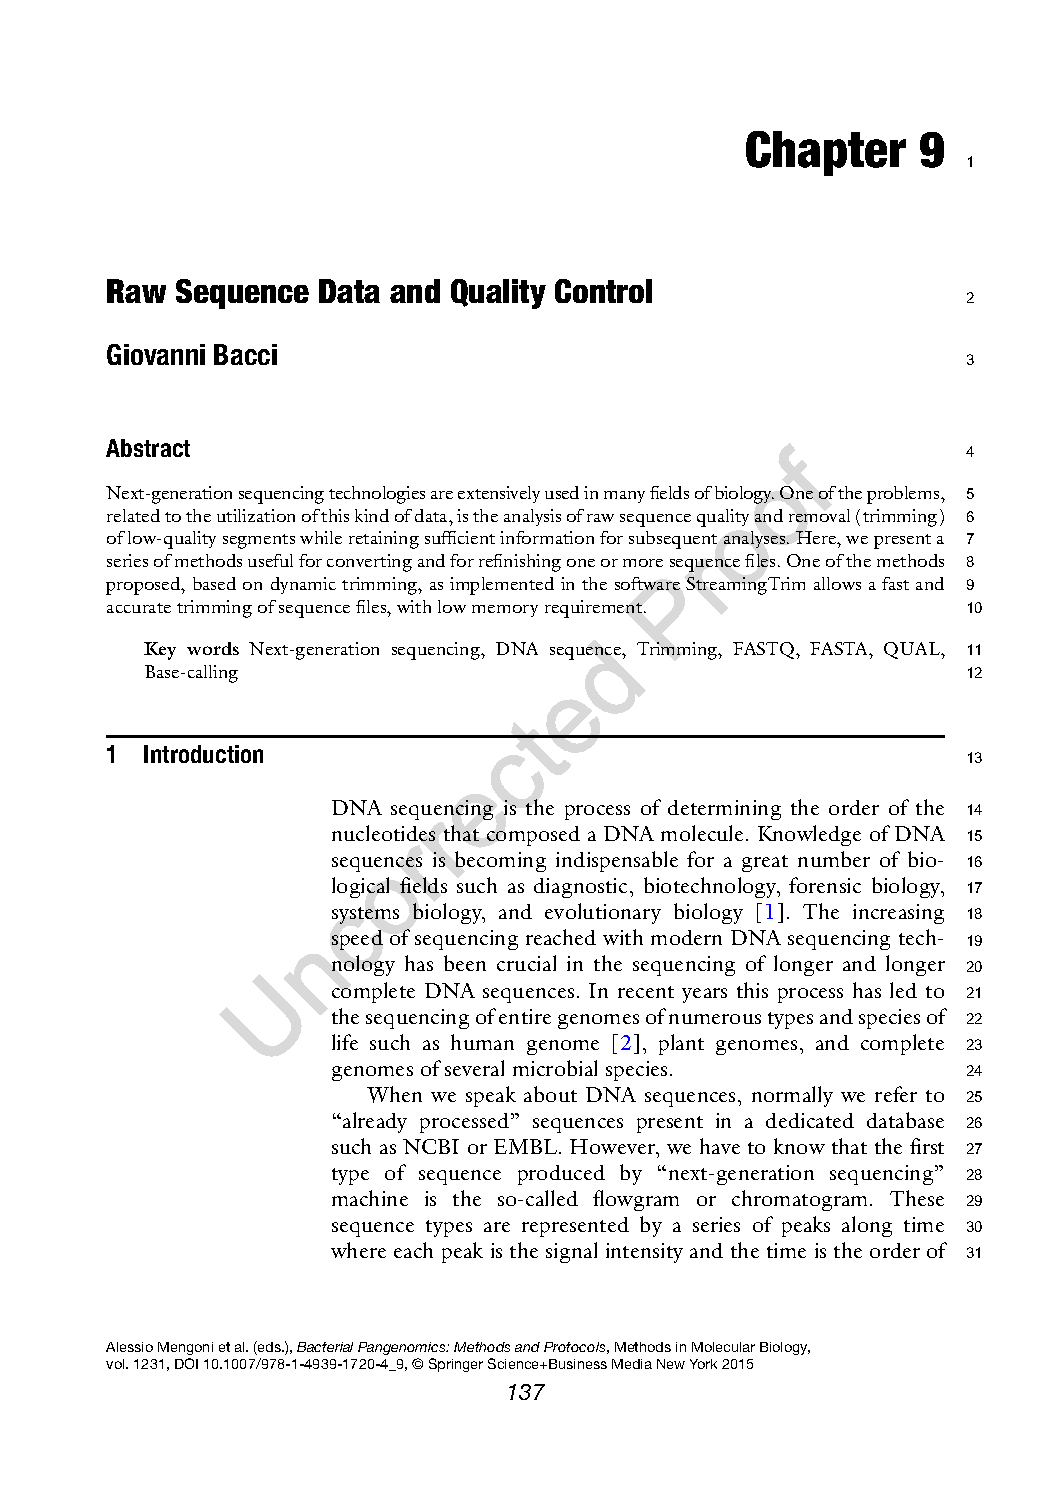
\includepdf[pages=-,offset=10mm 0, scale=0.9]{articles/book.pdf}
\newpage

\section[Evaluation of the performances of Ribosomal Database Project (RDP) Classifier for taxonomic assignment of 16S rRNA metabarcoding sequences generated from Il\-lu\-mi\-na-So\-le\-xa NGS]{Evaluation of the performances of Ribosomal Database Project (RDP) Classifier for taxonomic assignment of 16S rRNA metabarcoding sequences generated from Il\-lu\-mi\-na-So\-le\-xa NGS%
\sectionmark{Evaluation of the performances of RDP Classifier}}
\sectionmark{Evaluation of the performances of RDP Classifier}

Here we report a benchmark of the effect of bootstrap cut-off values of the RDP Classifier tool in terms of data retention along the different taxonomic ranks by using Illumina reads. Results provide guidelines for planning sequencing depths and selection of bootstrap cut-off in taxonomic assignments.\\

\subsection{Introduction}
The use of 16S rRNA massive sequencing has deeply improved the technical possibilities to describe the taxonomic composition and functionality of microbial communities \cite{degnan2011illumina}. Following the reduction in DNA sequencing cost, many studies have been performed using amplicon libraries to taxonomically describe microbial communities in many different environments. The large number of sequence reads can be taxonomically assigned by comparison with taxonomically classified sequences present in dedicated databases of 16S rRNA genes, as for instance SILVA \cite{quast2012silva}, Greengenes \cite{desantis2006greengenes} or the Ribosomal Database Project \cite{wang2007naive}. In particular, one of the most popular tool used to assign sequence reads to the prokaryotic taxonomy is the Na\"ive Bayesian Classifier tool hosted by Ribosomal Database Project (RDP Classifier) \cite{wang2007naive}. The RDP Classifier tool uses a very fast algorithm, based on the Bayes' theorem, suitable for the analysis of large amount of sequence data. This algorithm has been tested on near-full-length 16S rRNA sequences and on randomly generated 16S rRNA sequence fragments of 400, 200, 100 and 50 bases in length from a number (5,014) of type strains belonging to 988 genera \cite{wang2007naive}. An overall accuracy of above 88.7\% and 83.2\% for 400 and 200 base segments, respectively (very similar to the accuracy obtained with the near-full-length 16S rRNA sequence) was reported \cite{wang2007naive}. Moreover, an average accuracy at genus level of 71.1\% and 51.5\% for the 100 and the 50 base segments respectively was found. However, these results have been obtained using a 16S rRNA sequence fragments dataset built with sequences derived from well taxonomically defined organisms. No data have been reported on datasets composed by 16SrRNA sequences from particular regions of the 16S molecule (e.g. V3 and V6) and obtained after amplification of DNA from environmental samples. \\
In the last years, Illumina sequencing technology has emerged as one of the most popular sequencing technology, thanks to the lower prices, higher number of generated sequences and accuracy than pyrosequencing and Ion Torrent technologies \cite{degnan2011illumina, gloor2010microbiome, bartram2011generation, claesson2010comparison, salipante2014performance}. In particular, different Illumina platforms are available (with different cost of sequencing) which provide different number of reads and different reads lengths (see for instance \href{http://www.illumina.com/systems/sequencing.ilmn}{http://\-www.\-illumi\-na\-.com/\-sys\-tems/\-sequen\-cing\-.ilmn}). Additionally, Illumina reads are usually 100-200 nt long (depending on the techniques used) and 16S rRNA amplicon studies have focused on single variable regions of the 16S rRNA gene, as the V3, V4 or V6, which are approximately 100-300 bp long. Consequently, a concern about the amount of reads to generate and the setting of the bootstrap threshold of RDP Classifier to provide biologically meaningful data is present. More specifically, there is a lack of information on the percentage of reads which can be assigned to the various phylogenetic levels with Illumina 16S rRNA metabarcoding.\\

\subsection{Results and Discussion}
Here, we report a benchmark of RDP Classifier based on environmental sequence datasets obtained with Illumina sequencing technology. In particular, we investigated the effect of bootstrap cutoff values on the accuracy of taxonomic attribution of Illumina reads. Results obtained provide a guideline for the selection of optimal bootstrap cutoff values in terms of data retention along the different taxonomic ranks.\\
\begin{table}
\centering
\scriptsize
\begin{tabular}{ p{0.12\textwidth} p{0.06\textwidth} p{0.06\textwidth} p{0.06\textwidth} p{0.08\textwidth} p{0.4\textwidth} }
\hline
BioProject & Region & Length & Samples & Sequences & Environment\\
\hline\hline
PRJEB6047 & V3 & 302bp & 72 & 61023 & Subgingival, supragingival, and tongue plaque from healthy and periodontal subjects \\
PRJNA245381 & V3 & 300bp & 100 & 28634 & Soil contaminated with increasing level of ionic Ag\\
PRJNA217938 & V4 & 288bp & 25 & 476230 & Samples from the surface to depth in Upper Mystic Lake, Winchester, MA\\
PRJNA238275 & V4 & 251bp & 6 & 759518 & Soil associated with the rhizosphere of the coffee plant (\textit{Coffea canephora}) in Brazil\\
PRJNA188383 & V6 & 200bp & 48 & 66887 & Seawater and surface sediments retrieved from the Arctic Ocean\\\hline 
\end{tabular}
\caption{\label{tab:1rdp}Description of the datasets used. ``BioProject'' = accession ID (\href{http://www.ncbi.nlm.nih.gov/bioproject/}{http://\-www.\-ncbi.\-nlm.\-nih\-.gov/\-biopro\-ject/}); ``Region'' = rRNA gene variable region; ``Lenght'' = average read length; ``Samples'' = number of samples; ``Sequences'' = average number of sequences per sample; ``Environment'' = the environment where the study has been conducted.}
\end{table}
Five datasets of 16S rRNA gene Illumina reads, generated from environmental DNA, were analyzed (Table~\ref{tab:1rdp}). These datasets contains a high number of reads per sample (from 28,634 to 759,518 reads per sample) and are including reads obtained from V3, V4 and V6 regions.. Reads present in the analyzed datasets were trimmed with StreamingTrim version 1.0 [9], before taxonomic assignment with the RDP Classifier. The proportion of assigned reads in relation to the bootstrap cutoff value (from 0.1 to 1.0 with an increment of 0.1) for each taxonomic level (from \textit{domain} to \textit{genus}) is reported in Figure~\ref{tab:1rdp}. As expected, the proportion of assigned reads decreased going down along taxonomic levels from \textit{phylum} (from a mean of 100\% to a mean of 25\%, in the two datasets) to \textit{genus} (from a mean of 60\% to a mean of smaller than 5\%, in the two datasets). In particular it is worth noticing that all datasets, which included three variable regions (V3, V4 and V6) of 16S rRNA gene, more than 25\% of the reads could be assigned to the family level using a bootstrap cutoff value of 0.5 (the default cut-off value reported in the RDP Classifier tutorial). Moreover, even at higher cutoff values ({\textgreater} 0.8) an appreciable number of reads were still assigned (5\% - 10\%). Interestingly, the V3 region performed better in the taxonomic attribution at Order and Family levels, indicating that even highly stringent bootstrap cut-off values (e.g. 0.7) may allow to assign more reads from V3 region than from V4 and V6 region, which consequently resulted less taxonomically informative.\\%
\begin{figure}[!tb]
	\centering
	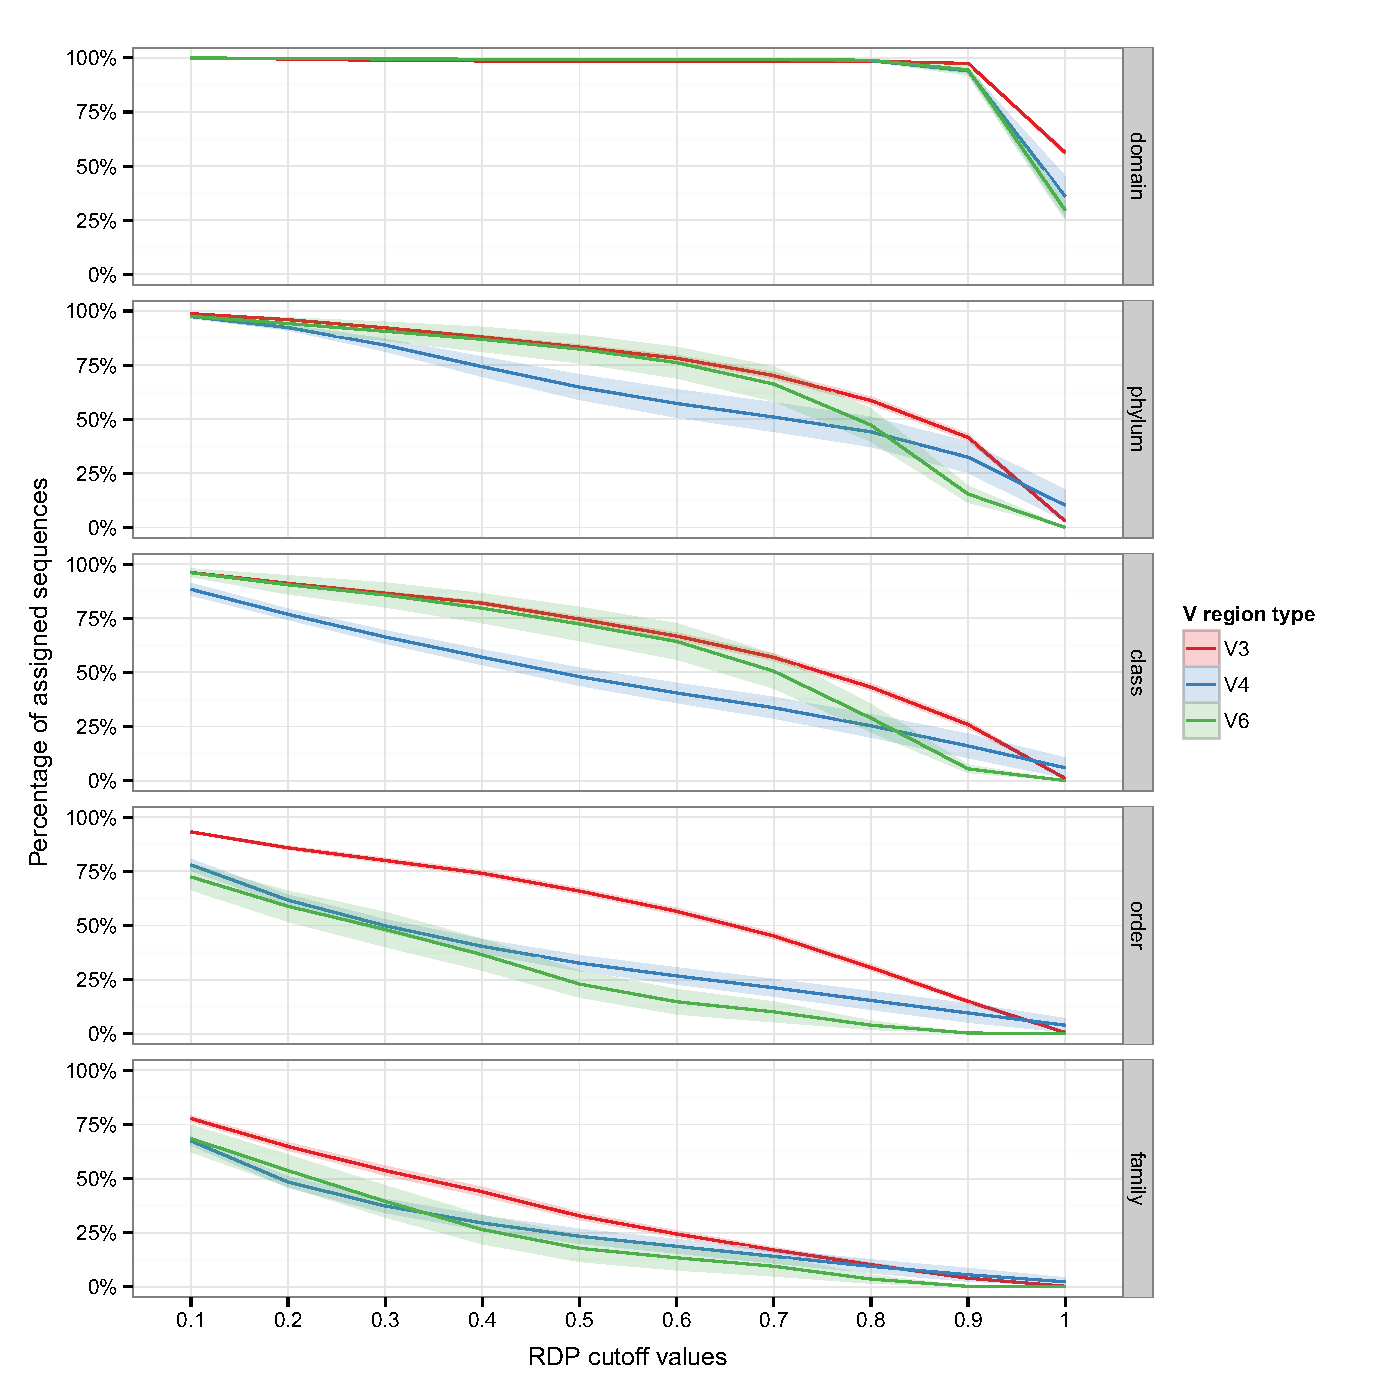
\includegraphics[width=0.8\textwidth]{./figures/Chapter_2/Figure_1}
  	\caption{\label{fig:1rdp}Effect of bootstrap cut-off thresholds on the number of reads. The percentage of trimmed reads assigned to each taxonomic level is reported versus RDP bootstrap cut-off values. Shaded lines correspond to the 95\% confidence interval assuming normality.}
\end{figure}%
The assignments trend at the \textit{genus} level (the lower taxonomic level that can be obtained using the RDP Classifier) was then inspected (Figure~\ref{fig:2rdp}).  Here also, V3 region better performed than V4 and V6 region in the retention of taxonomic information lowering bootstrap values, especially at bootstrap cutoff value of 0.5 and lower. A pseudo-fit of curve was also produced (Supplemental Figure SM1), which may allow researchers to infer the percentage of sequences that could be assigned to the \textit{genus} level at different RDP bootstrap cut-offs.\\%
\begin{figure}[!tb]
	\centering
	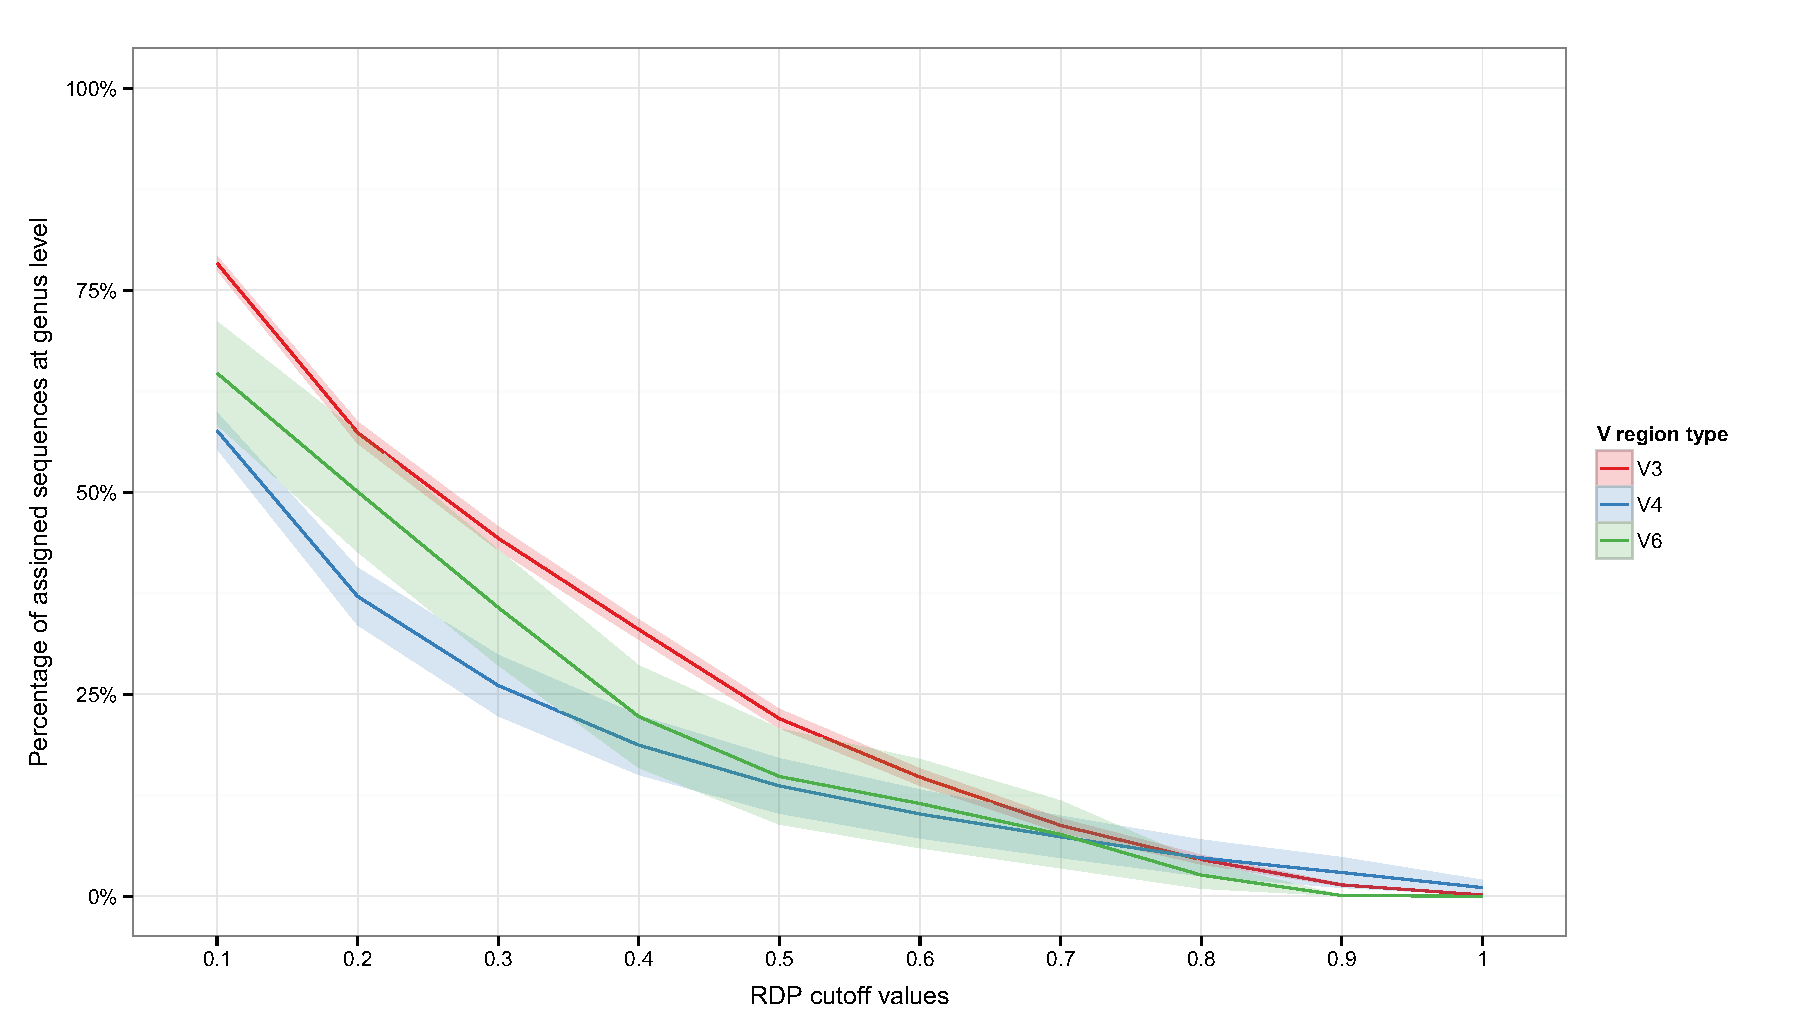
\includegraphics[width=0.8\textwidth]{./figures/Chapter_2/Figure_2}
  	\caption{\label{fig:2rdp}Percentage of assigned reads with respect to bootstrap cut-off thresholds at the genus level. Plots report the assigned reads for all dataset analyzed. Shaded lines correspond to the 95\% confidence interval assuming normality.}
\end{figure}%
In conclusion, Illumina reads, shorter than 200 nt, can be classified using one of the most common 16S rRNA sequence classifier: the RDP Classifier. As one would expect, the increase of the bootstrap cutoff value leads to a decreased number of assigned sequences. However, even at cutoffs higher than those indicated in the RDP Classifier tutorial, approximately 20-30\% of the analyzed reads were still assigned. These results indicate that Illumina-based metabarcode sequencing of 16S rRNA gene can provide reliable information for taxonomic composition of a community at the genus level even using classification software not specifically designed for this type of sequences. The reported models for trend plots can guide experimentalists in choosing the sequencing depth more adapted for retaining an appreciable number of assigned reads different taxonomic resolution.\\

\subsection{Acknowledgments}
This work was supported by a grant from the Ente Cassa di Risparmio di Firenze (Grant n{\textdegree} 2010/4384 ``Centro di Metagenomica del suolo'') and by a fellowship to GB from MIPAAF.

\section[StreamingTrim 1.0: a Java software for dynamic trimming of 16S rRNA sequence data from metagenetic studies]{StreamingTrim 1.0: a Java software for dynamic trimming of 16S rRNA sequence data from metagenetic studies%
\sectionmark{StreamingTrim 1.0}}
\sectionmark{StreamingTrim 1.0}

The so-called barcode or metagenetic applications, based on PCR amplicon library sequencing, are very popular at present time. One big problem, related to the utilization of amplicon data, is the analysis of reads quality and the removal of low-quality regions without deleting entire sequences which can be useful for subsequent analyses (e.g. taxonomic assignment). Here, we present StreamingTrim, a DNA reads trimming software, written in Java, that allows researchers to analyse the quality of DNA sequences in fastq files searching and removing low-quality regions in a very conservative way.\\
\newpage
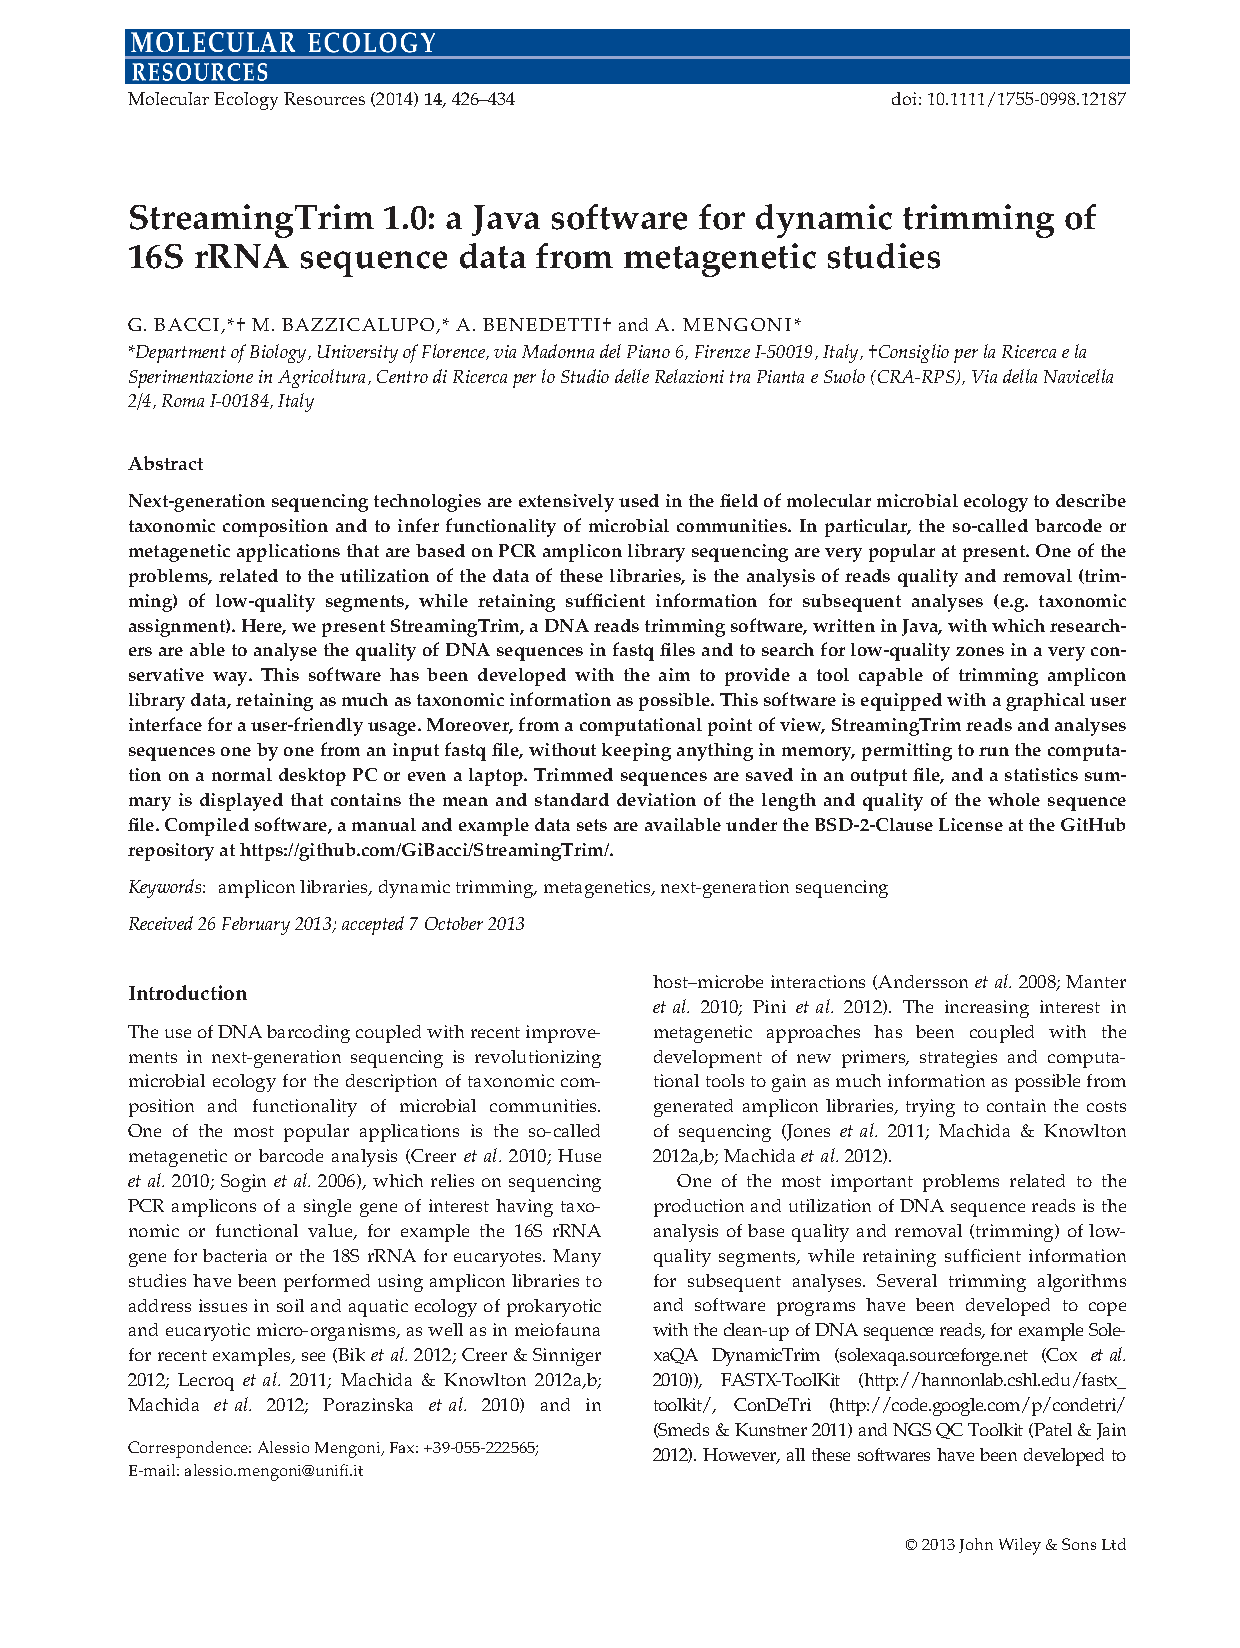
\includepdf[pages=-,offset=10mm 0, scale=0.9]{articles/StremingTrim.pdf}
\newpage

%%-----------
%% Backmatter
%%-----------
\backmatter
\chaptermark{Bibliography}
\renewcommand{\sectionmark}[1]{\markright{#1}}
\bibliographystyle{unsrt}                           %Use alpha codes for references
\sectionmark{Bibliography}
\addcontentsline{toc}{chapter}{Bibliography}        %Force addition of Bibliography to TOC    
\bibliography{References}								

\mainmatter
\newthumb
%%%%%%%%%%%%%%%%%%%%%%%%%%%%%%%%%%%%%%%%%%%%%%
\logvartrue
\chapter{Bacteria-environment interaction}
%%%%%%%%%%%%%%%%%%%%%%%%%%%%%%%%%%%%%%%%%%%%%%
Microscopic bacteria are usually considered one of the most simple and primitive living species. In the popular mind, they are associated almost exclusively with infection diseases or with the bio-degradation of organic matter. But reality is different, hence, within a highly diversified and beneficial bacterial world, only a very small fraction is able to cause infections. Most of known bacterial ``species'' reciprocally support each other and are able to define and sustain a balanced environment, the so-called biosphere. This ``solidarity'' among bacterial cells is one of their  most important characteristics. Indeed, even pathogenic bacteria are able to benefit from these mutual interactions, helping themselves to be more flexible than if they lived as isolated species. For these reasons studying the relations between bacteria and their environment by identifying their community structure is becoming more and more considered as a mandatory step towards the comprehension of the biological dynamics existing on our planet.\\
These topics have been discussed in the following paper:
\vspace{-5mm}
\begin{itemize}[nosep]
\item \textbf{Bacci, G.}, Ceccherini, M.T., Bani, A., Bazzicalupo, M., Castaldini, M., Galardini, M., Giovannetti, L., Mocali, S., Pastorelli, R., Pantani, O.L., Arfaioli, P., Pietramellara, G., Viti, C., Nannipieri, P., \& Mengoni, A. Exploring the dynamics of bacterial community composition in soil: the pan-bacteriome approach.
\end{itemize}
which has been submitted for publication to \textit{Antonie van Leeuwenhoek}.

\section{Exploring the dynamics of bacterial community composition in soil: the pan-bacteriome approach}
We performed a longitudinal study (repeated observations of the same sample over time) to investigate both the amount and structure of temporal changes of bacterial community composition in soil mesocosms, subjected to three different treatments (water and 5 mg kg\textsuperscript{-1}, 25 mg kg\textsuperscript{-1} of dried soil Cd\textsuperscript{2+}). By analogy with the pan genome concept, we identified a core bacteriome and an accessory bacteriome. Resident taxa were assigned to the core bacteriome, while occasional taxa were assigned to the accessory bacteriome. Core and accessory bacteriome represented roughly 35\% and 50\% of the taxa detected, respectively, and were characterized by different taxonomic signatures from phylum to genus level while the 15\% of the taxa were found to be unique of a particular sample. In particular, the core bacteriome was more abundant in members of \textit{Planctomycetes}, \textit{Actinobacteria}, \textit{Verrucomicrobia} and \textit{Acidobacteria}, while the accessory bacteriome included more members of \textit{Firmicutes}, \textit{Clamydiae} and \textit{Proteobacteria}, suggesting potential different responses to environmental changes of members from the such phyla. We conclude that the pan-bacteriome model may be a useful approach to gain insight for modelling bacterial community structure and inferring different abilities of bacteria taxa.\\

\subsection{Introduction}
Understanding changes in bacterial community structure over time is still one of the major challenges in microbial ecology \cite{ge2008differences, zhou2014stochasticity, donn2014evolution}. Indeed, environmental changes often affect taxonomic composition and taxa abundance in microbial communities \cite{allison2008resistance}, which may have strong effect on soil health and plant productivity \cite{chaparro2012manipulating}. Several works have been performed inspecting bacterial community variation both in cross sectional (different sites at the same time) and longitudinal studies (the same site studied over time) \cite{costello2009bacterial, pini2012exploring, smith2012cervical, bartram2014exploring, logares2012biogeography, chen2013shifts, kuang2012contemporary}.\\
A pan-genome is defined as the collection of all the genes of a set of bacteria which can be divided into core genome (the group of genes shared by all the selected bacteria), accessory genome (the group of genes present in some, but not all, the selected bacteria) and unique genome (genes belonging to only one particular bacteria) \cite{tettelin2008comparative}. In analogy with this concept we can define a pan-bacteriome as the collection of all bacterial taxa present in a set of environmental samples. As recently reported \cite{hardoim2014temporal}, the pan-genome, even the pan-bacteriome can be divided into core bacteriome (the pool of taxa shared by all the samples), accessory bacteriome (the group of taxa found in some, but not all the samples) and the unique bacteriome (taxa detected only in a particular sample).\\
Several recent works \cite{bartram2014exploring, logares2012biogeography, bowen2012salt, aravindraja2013ultradeep, dohrmann2012importance, gibbons2013evidence, kim2013general, oh2013altered, portillo2013cell, sanchez2013assessing, szekely2014importance, wegner2013disturbance}, mainly performed with next generation sequencing technologies, have demonstrated that most bacterial communities are composed of a few abundant taxa and a plethora of rare ones \cite{pedros2012rare}. Such different fractions may have in theory different taxonomic signatures (at the various taxonomic levels), in relation to the physiological features of the groups of taxa present. For these reasons, we define the ``pan-bacteriome'' concept, as the whole set of taxa present in a bacterial community analyzed through multiple samplings along time. The pan-bacteriome will then include both a core and an accessory fraction, which describe the taxa shared by all samples and the taxa present only in some samples, respectively. In addition, the so called ``rare biosphere'', composed by taxa occurring only in a fraction of the community samples, and interpreted as the accessory fraction of the bacterial community, seems more readily respond to environmental changes \cite{dohrmann2012importance, kim2013general, szekely2014importance, campbell2011activity, gobet2011diversity}.\\
Contaminated soils have been often used as models for inspecting bacterial evolution over time \cite{mengoni2010plants, porter2013trade}, since different bacterial taxa show different responses to contamination. The most oxidized state (and most frequent) of cadmium (Cd\textsuperscript{2+}) is known to be toxic for soil microbial biomass and activity \cite{renella2002cadmium, renella2005microbial} and several studies have shown that Cd\textsuperscript{2+} concentrations affect soil microbial genetic diversity under short-term cadmium stress \cite{gomes2010effects, lorenz2006response, chien2008microbial, duan2008effect, lazzaro2008identification, sheoran2008remediation, zhang2009responses, fritze2000effect}. The aim of this work was to apply the pan-bacteriome model, as sum of a core and an accessory assemblage of bacteria taxa present in bacterial communities, to evaluate the dynamics of bacterial community composition in three soil mesocosms, exposed to slightly different environmental conditions (concentrations of 0, 5 mg kg\textsuperscript{-1} and 25 mg kg\textsuperscript{-1} of dried soil Cd\textsuperscript{2+}) along time. A metabarcoding approach was applied on 16S rRNA gene based on Illumina sequencing technology.\\

\subsection{Materials and Methods}

\subsubsection{Experimental setup}
The top layer (0-15 cm) of a soil located near Romola (Florence, Italy 43.696240 N, 11.153894 E) was sampled (about 20 kg), air-dried overnight at room temperature and sieved at 2 mm. The sieved air-dried soil mass was repeatedly splitted to ensure the representativeness of the initial material, which resulted finally divided into masses of about 1 Kg each. One mass was analyzed for relative humidity (RH 7.30\%), particle size (sand 81.9\%; silt 6.7\%; clay 11.4\%), water holding capacity (WHC 14.85 g 100 g\textsuperscript{-1} of dried soil), pH (5.4), total organic C (0.7\%), total organic N (0.07\%) after the air-drying process and just before the constitution of the mesocosms.\\
Three of the remaining masses were used to constitute the mesocosms. Each mesocosm was formed by a flat-bottomed plexiglas cylinder (10 cm height, 15 cm of diameter) previously disinfected with 70\% ethanol, which contained the soil mass. Its base was perforated to permit aeration and water flow. The cylinder was supported by a similar one not perforated, intended to collect any possible leak of soil or solution. The upper part of the mesocosm was weighted, to keep track of the water losses which were reconstituted weekly throughout the experiment. Then an excess 350 ml of sterile distilled water was thoroughly and slowly dripped on the dried soil: the mesocosms were then brought to a thermostatic clean room at 22 {\textdegree}C into which they were maintained and their position rotated every third day for two months. When the mesocosms reached about the 25\% of the WHC, they were randomly assigned to one of the following treatment: A) sterile distilled water, B) 3CdSO\textsubscript{4}{\textperiodcentered}8H\textsubscript{2}O (Sigma-Aldrich) sterile solution as to reach a final concentration of 5 mg kg\textsuperscript{-1} of dried soil, C) 3CdSO\textsubscript{4}{\textperiodcentered}8H\textsubscript{2}O sterile solution as to reach a final concentration of 25 mg kg\textsuperscript{-1} of dried soil (Figure SM1). The volume and the concentration of Cd solutions were adjusted to reach both the 50\% of the soil WHC and the Cd concentration in mg kg\textsuperscript{-1} of dried soil. The mesocosms were sampled at 0, 1, 4, 8, 36 and 60 days (t0, t1, t4, t8, t36, t60) after the initial Cd solution spiking. The first sampling time (t0) took place as soon as the Cd solution was visibly soaking the whole soil mass. On each date, a brass pipe was used to withdraw three replicates. DNA extraction was performed on each of the three soil cores (1.2 cm diameter, 6 cm deep). The location of the cores on the mesocosm surface was selected by randomly generating 1000 groups of 6 {\texttimes} 3 polar coordinates (i.e. an angle and a distance for each date and replica): if the area of the cores in two or more locations/dates overlapped or were tangent, the next group (among the 1000 generated) with more distant locations was selected. An R script was used to generate and print 1000 cardboard notched disks which were used to unambiguously locate the position of the cores, as previously described \cite{ceccherini2007effect}. A total of 54 samples (3 mesocosms, 6 sampling dates, 3 soil cores for DNA extraction (replicates) were collected (Figure SM1). All steps were performed under sterile  conditions.\\

\subsubsection{DNA extraction and 16S rRNA metabarcoding}
Each soil core was well amalgamated (mixed) before DNA extraction. DNA was extracted from 0.5g of the cores using the bead-beating method as previously described \cite{ascher2009sequential}. The extracted DNA was checked by electrophoresis on 1\% (w/vol) agarose gel and quantified by Picodrop spectrophotometer (Picodrop Limited, UK).\\
For metabarcoding, each extracted DNA sample was amplified using specific primers for the variable V6 region of 16S rDNA (V6-967F 5'-CAA\-CGC\-GAA\-GAA\-CCT\-TAC\-C-3' and V6-1046R 5'-CGA\-CAG\-CCA\-TGC\-ANC\-ACC\-T-3' \cite{huse2008exploring}. PCR conditions were those previously described by Sogin and co-workers \cite{sogin2006microbial}. Ten independent PCR reactions for each of the 54 samples were done. Products were resolved by agarose gel (1.5\% w/vol) electrophoresis and bands were purified with MinElute Gel Extraction Kit (Qiagen, Inc.). Quality and quantity of products were assessed spectrophotometrically (Biophotometer, Eppendorf). The obtained amplicons from each sample were pooled together and a total of 54 samples were sequenced. Massive sequencing was performed by Illumina-Solexa technology \cite{bartram2011generation,gloor2010microbiome} with the pair-end protocol on an Illumina HiSeq2000 machine by Beijing Genome Institute sequencing service \href{www.genomics.cn}{www.\-gen\-omi\-cs.cn}. Sequences are deposited in SRA database under the BioProject accession number SRP038532.\\

\subsubsection{Bioinformatic processing of 16S rRNA metabarcoding data: data pretreatment}
Sequences were analyzed in order to identify and remove any low quality regions. Since raw sequences had a length of 100 bp, the quality control step had to be very conservative, to prevent the removal of many taxonomically significant data. As a consequence, a dynamic trimming algorithm was used \cite{bacci2014streamingtrim} setting the cutoff parameter as the mean quality of the whole files minus the standard deviation value (in this case an average quality cutoff of 33 Phred was used for all files \cite{ewing1998base, ewing1998base}). Collected sequences were subjected to a further quality control step and assembled using PANDAseq \cite{masella2012pandaseq}. Finally, a set of 18,778,601 sequences (mean length 112 bp and overlapping for more than 70 bp, data not shown) was achieved and used for successive analyses. In order to assign each read to specific taxa we used the RDP multiclassifier trained on the default RDP dataset (16S training set 9). An assignment cutoff of 0.5 was used as reported in the RDP Classifier pipeline for sequences shorter than 250 bp \cite{wang2007naive}.\\

\subsubsection{Data treatment and statistical analysis}
RDP assignments at all taxonomic levels (from Phylum to Genus) were collected. The average number of assignments in all samples has been evaluated to detect biased samples (samples with an inconsistent number of assignments). RDP assignments were collected for each sample to generate a community data matrix (\textit{X}) at genus level (rows = samples; columns = detected genera) (Table SM1). \textit{X} was used as the input/source for all statistical analyses. In order to detect genera belonging to the core and to the accessory bacteriome, \textit{X} was transformed into a Boolean (presence/absence) matrix (\textit{X}\textit{\textsubscript{p/a}}). Abundance values greater than or equal to 1 were rounded to 1 while abundance values equal to 0 were left unchanged. Each genus was assigned to one of the core or to the accessory bacteriome fractions using these criteria: if a genus was detected in all samples (its abundance value was greater than 0 in the 54 samples) it was assigned to the core bacteriome; otherwise it was assigned to the accessory bacteriome. In addition, if a genus was detected only in a single sample, it was considered as ``unique assignment''.\\
To assess taxa richness, a rarefaction analysis was performed using the R package Vegan \cite{oksanen2007vegan, dixon2003vegan}, based on the genus assignments in \textit{X}. The variation in the composition of bacterial communities with respect to conditions and time was analyzed by canonical correlation analysis (CCA) using the R package Vegan on \textit{X}. The different conditions and the sampling times have been fitted onto previously developed ordination analyses using the \textit{envfit} function of the R package Vegan with 10'000 permutations.\\

\subsection{Results}

\subsubsection{Description of sequence data and coverage}
A total of 18,778,601 reads were processed for the 54 sequence files representing each of the samples (Figure SM1). The reads in the sequence files ranged from a minimum of 339,328 to a maximum of 356,164. A preliminary analysis showed that the percentage of reads assigned to each taxonomic level was similar (standard error {\textless} 0.001) among all files and that a mean of 39.6\% of total reads was assigned to the genus level (Figure~\ref{fig:1rom}), with a total of 901 genera (with a similarity cutoff of 95\%). To describe the richness of the samples at genus level, a rarefaction analysis has been performed (Figure~\ref{fig:2rom}). Since the curves reached slope values near 0,  the richness of each sample was uniform regardless of simulated environmental conditions or sampling time. Finally, an analysis of similarities (ANOSIM) was performed using all genus assignments in matrix \textit{X} (Table SM1) as response variables. Both conditions and sampling times were used for grouping together samples from the same replicate (see Figure SM1). As a result, the ANOSIM analysis has shown that samples belonging to the same triplicate differed significantly between each group (p-values {\textless} 0.05 obtained with the \textit{anosim} function from R package \textit{vegan}, Figure SM2). When calculating the diversity indices (Richness, Shannon and Simpson index) also, all samples showed similar values (Table SM2).\\
\begin{figure}[!tb]
	\centering
	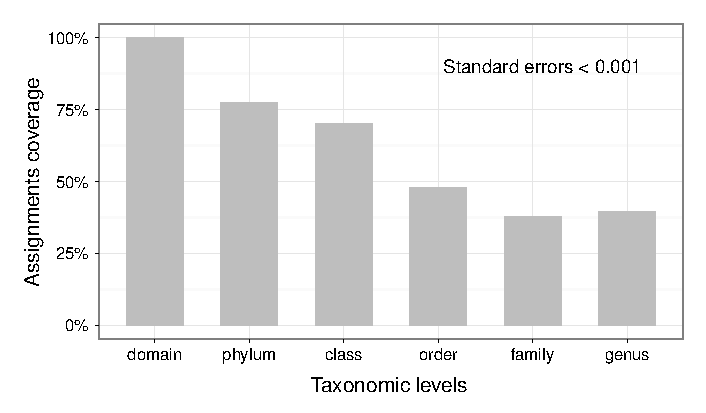
\includegraphics[width=0.7\textwidth]{./figures/Chapter_3/Fig1.eps}
  	\caption{Percentage of reads assigned at each taxonomic level. The number of reads assigned at each taxonomic level has been calculated for each sample. The average number of assigned reads for each taxonomic level from Phylum to Genus is reported. The standard error is shown at the top right of the plot. \label{fig:1rom}}
\end{figure}

\begin{figure}[!tb]
	\centering
	\includegraphics[width=0.8\textwidth]{./figures/Chapter_3/Fig2.eps}
  	\caption{Rarefaction curves. Reported curves have been created by randomly re-sampling the pool of assignments for each sample multiple times and then plotting the average number of genera found in each sample. An increasing step of 1000 assignments has been chosen in order to draw smooth curves. The slopes of each step has been calculated for each sample and reported in the top panel while rarefaction curves have been reported in the bottom one. \label{fig:2rom}}
\end{figure}

\subsubsection{Differential taxonomic assemblage in core and accessory bacteriome}
To check whether the differences found in the composition of the bacterial community at genus level were also represented at higher taxonomy levels (Table SM3), all genus assignments were collected and collapsed from Phylum level to Order level. Then, taxonomic differences between core and accessory bacteriomes were inspected (Figure\ref{fig:5rom}). Beginning from Phylum level, core and accessory groups displayed significant differences in almost all phyla (only 2 phyla out of 23 did not differentiate between the two groups). In particular, six phyla (\textit{Gemmatimonadetes}, \textit{Elusimicrobia}, OD1, TM7, WS3) were only detected in core bacteriome, as well as other six phyla (\textit{Cyano\-bacteria}, \textit{Aquificae}, \textit{Deino\-coc\-cus\--Ther\-mus}, \textit{Fuso\-bacte\-ria}, \textit{Lenti\-sphaerae}, OP11) were present in accessory bacteriome only. The presence of such phyla exclusive of the two pan- acteriome fractions highlight the presence of large taxonomic differences between them, which was also clear from a higher abundance of members of \textit{Plancto\-mycetes}, \textit{Actino\-bacteria}, \textit{Verruco\-micorbia} and \textit{Acido\-bacteria} in the core bacteriome, while the accessory bacteriome comprised more member of \textit{Firmicu\-tes}, \textit{Clamy\-diae} and \textit{Proteo\-bacteria}. Similar results were obtained by inspecting different taxonomic assemblage at Class level. In fact, 16 classes out of 19 showed different occurrences between core and accessory bacteriomes, with 4 (\textit{Erysi\-pelotri\-chia}, \textit{Epsilo\-proteo\-bacteria}, \textit{Holo\-phagae}, Subdivision 5) and 2 (\textit{Acido\-bacteria}, Subdivision 3) classes only present in the accessory and in the core bacteriome, respectively. Finally, almost all detected orders showed a differential occurrence patterns between accessory and core bacteriome, with 7 orders found exclusively in the core dataset and 12 orders found exclusively in the accessory dataset.\\
\begin{figure}[!tb]
	\centering
	\includegraphics[width=1\textwidth]{./figures/Chapter_3/Fig5.eps}
  	\caption{Phylogenetic dissection of variation of core and accessory bacteriome. Heatmaps report the difference of each taxonomic assignment between the core and the accessory bacteriomes. Differences have been tested using a t-test (with the exclusion of presence/absence patterns). Colors are reflecting the level of the related genus in the heatmap. Green and red colors correspond to high and low abundances values, respectively. The asterisks indicate the p-value threshold in each comparison (one asterisk indicates a p-value lower than 0.05 but higher than 0.001 while two asterisk indicates a p-value lower than 0.001). The open circle indicates a strict presence/absence. \label{fig:5rom}}
\end{figure}
Finally, to give an insight into the different genera distribution inside each sample (Table SM4), the number of sequences attributed to each genus was transformed into a relative abundance value. These values were used to display bacterial taxonomic composition in each sample and in each bacteriome (Figure~\ref{fig:6rom}). Results confirmed the overall representation of a conserved core group and of a more scattered accessory genera distribution. Moreover, from this analysis the core group seemed to vary (a little) in relation to the sampling time while, the accessory bacteriome displayed a variation with respect to sampling time to treatment and among repetitions.\\
\begin{figure}[!tb]
	\centering
	\includegraphics[width=1\textwidth]{./figures/Chapter_3/Fig6.eps}
  	\caption{Relative abundances of genera detected in the core and accessory bacteriomes. Color patterns refer to distinct
901 genera (see Table SM1). In the two panels, abundance values for the core bacteriome and the accessory bacteriome are
reported on the left and the right, respectively. A, B and  C refer to the three treatments. \label{fig:6rom}}
\end{figure}

\subsubsection{Defining core and accessory bacteriome}
In order to describe the bacterial community structure of the soil under study, considering all samples the \textit{X} matrix was transformed using the logarithmic function. Thus, a heat map was produced displaying the abundance of all genera in the samples (Figure~\ref{fig:3rom}, Table SM4), which indicated the presence of high represented and shared taxa (red regions over the whole map) and of occasional taxa (regions of the heat map that do not display a uniform color inside the plot). These groups of taxa were defined (as detailed in the Materials and Methods section) as core and accessory bacteriome, respectively. The core (shared) set of genera included those present in all samples (without considering changes in their abundance), while the accessory bacteriome included those genera not present in all samples.\\
\begin{figure}[!tb]
	\centering
	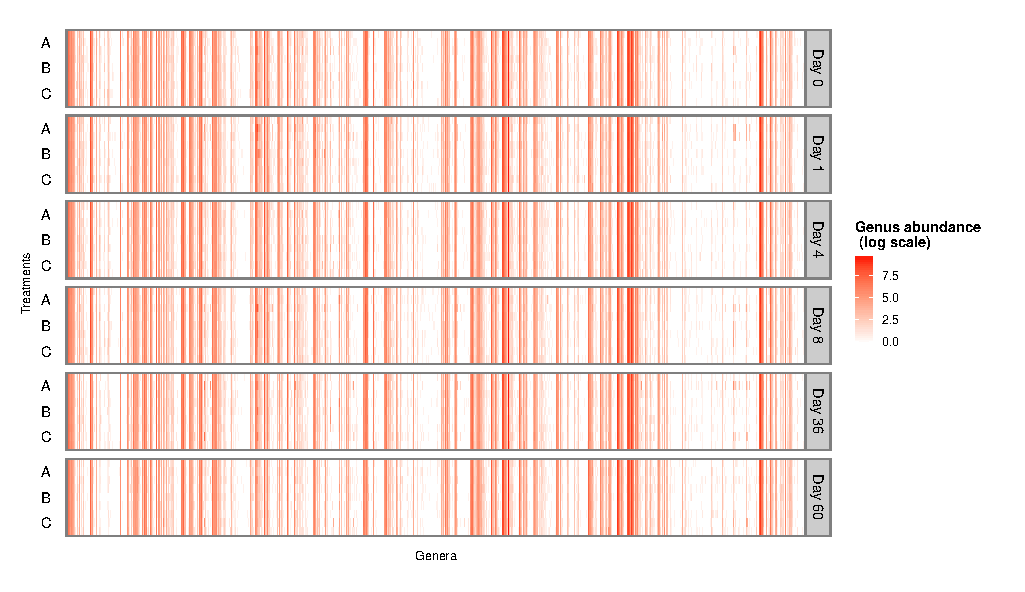
\includegraphics[width=1\textwidth]{./figures/Chapter_3/Fig3.eps}
  	\caption{Bacterial community structure at genus level. The number of assignments at genus level has been transformed using the logarithmic function in order to reduce the range of values. The obtained values have been reported using a heat map representation. As reported in the plot, red color represents high number of assignments (10\textsuperscript{7}), while the white color indicates a low number of assignments (below 10\textsuperscript{1}). Samples have been divided into six blocks following sampling time (grey blocks to the right). Each block has been divided into 9 lines, grouped into three parts following the three simulated environmental conditions (named A, B and C, corresponding to water, Cd 5 mg/kg and 25 mg/kg, respectively). The 901 genera identified in the samples were ordered according to the taxonomic output of RDP Classifier (see Table SM2). \label{fig:3rom}}
\end{figure}
In terms of number of classified reads, the core and the accessory bacteriome contained 99.4\% and 0.5\% of all sequences classified at genus level, respectively (data not shown). Furthermore, 120 genera were detected in one sample only (less than 0.1\% of the whole sequences); these genera were considered as ``unique'' ones and were excluded from the following analysis (Table SM4). Regarding the core and the accessory bacteriome fractions we have collected 316 core genera (35.1\% of the total)and 465 accessory genera (51.6\% of the total) (Figure~\ref{fig:4rom}).\\
\begin{figure}[!tb]
	\centering
	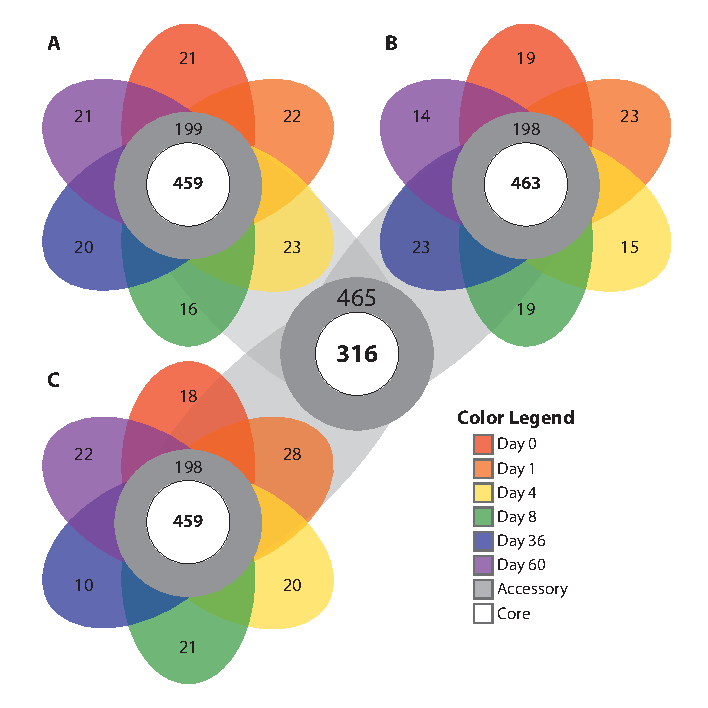
\includegraphics[width=0.7\textwidth]{./figures/Chapter_3/Fig4.eps}
  	\caption{The pan-bacteriome size. Pseudo-Venn diagrams drawn for each treatment dividing each sample according to sampling time. Generated plots report the number of genera found only at a specific time (unique assignments), the number of genera detected at least at two distinct times (accessory assignments) and the number of genera detected in all samples regardless sampling time (core assignments). The two groups reported in the middle of the three Venn diagrams are the accessory and the core groups defined with respect to the whole bacterial community, regardless sampling time and treatment. The three Venn diagrams marked with the letters ``A'', ``B'' and ``C'' are referring to the 3 treatment conditions (0, 5, 25 mg/kg of Cd). \label{fig:4rom}}
\end{figure}

\subsubsection{Effect of sampling time and treatment on the whole pan-bacteriome components}
The last investigated questions relied on the differential sensibility of core and accessory bacteriome over bacterial community variations induced in when comparing the three different mesocosms (treatment A, B, and C, with [Cd\textsuperscript{2+}] at 0, 5 and 25 mg kg\textsuperscript{-1}, respectively). Two analyses were performed by CCA: one considering all samples collected for the analysis (replicates included) and one pooling the 3 replicates of each condition into a single observation. Both factors (sampling time and treatment) were fitted onto the two ordination analyses described above (Figure~\ref{fig:7rom}). Results showed a tendency of the non-pooled samples to preferably cluster based on sampling time rather than on treatments. On the other hand, the pooled samples displayed an opposite behavior; in fact, they tended to cluster following the treatments (A, B, C) but not the sampling time. These contrasting results could be due to the high level of heterogeneity in the accessory bacteriome assignments. As shown in the bacterial communities analysis performed above (Figure~\ref{fig:6rom}), the accessory group displays a very scattered bacterial distribution even inside the same temporal and treatment conditions. If this effect is minimized by pooling the 3 replicates inside a single sample even the effect of randomness is minimized. On the contrary, if this effect is not reduced, replicates of the same conditions result in a high degree of overlap in the ordination analysis.\\
\begin{figure}[!tb]
	\centering
	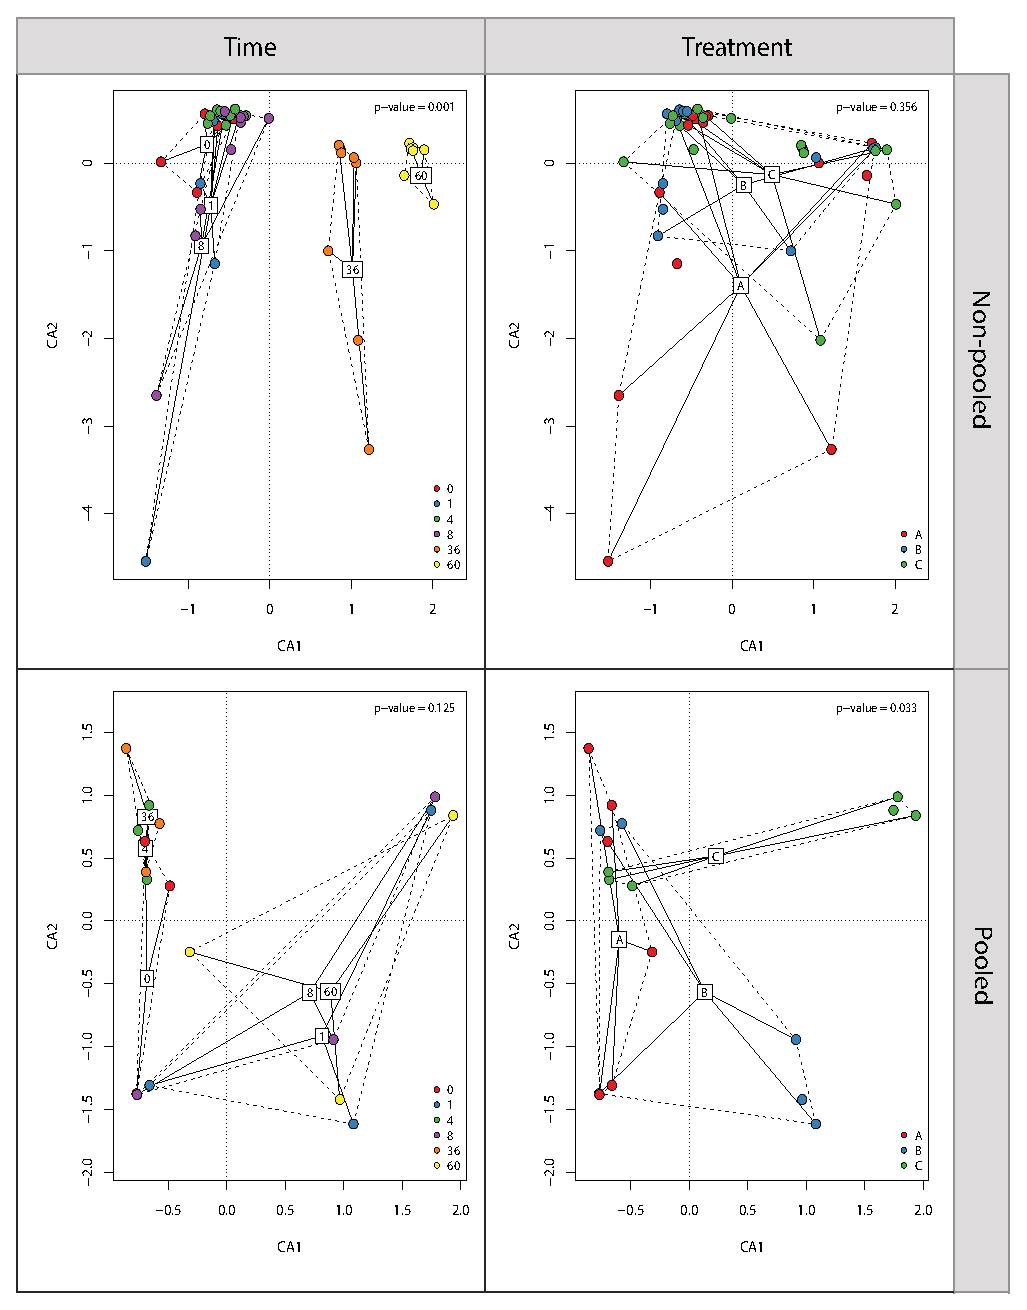
\includegraphics[width=0.9\textwidth]{./figures/Chapter_3/Fig7.eps}
  	\caption{Effect of environmental variables on the pan-bacteriome assemblage. Canonical Correlation Analysis of the whole bacterial community are reported. The four plots are divided according to the time and treatment factor (vertical division) and according to the dataset used (horizontal division). In particular, the two plots in the bottom panel report the ordination analysis based on the pooled dataset (samples with the same conditions were pooled together) whereas the two plots in the top panel report the ordination analysis based on the whole bacterial community (all samples). P values derived from an environmental fitting analysis onto the bacterial dataset where reported in the top right corner of each plot. \label{fig:7rom}}
\end{figure}

\subsection{Discussion}
It is now widely accepted that bacterial communities are composed by an assembly of resident taxa, those being slightly affected by environmental variables, and by occasional/fluctuating taxa, those varying among samples \cite{logares2012biogeography}. Often resident taxa are the most abundant, while occasional taxa tend to be rare \cite{gobet2011diversity}. Recently, habitat specialization has been used to classify and provide insight into the ecological behavior of microbial taxa \cite{szekely2014importance}.\\
To better describe the assemblage of bacterial communities as a sum of resident and occasional taxa, we have used a conceptual framework analogous to the pangenome concept \cite{tettelin2008comparative}, which is used for describing bacterial genomes belonging to the same species as sum of a common gene set (core genome) and of a dispensable/accessory gene set. In particular, we evaluated the presence of core and accessory bacteriomes in a set of three soil mesocosms followed over time.\\
The presence of two main fractions of the bacterial community was highlighted; one (the core), including the resident taxa while the other (accessory) composed of occasional taxa. The accessory taxa were by far less represented than the core taxa, considering the number of sequence assigned to each group. Since our experimental dataset included three different mesocosms (treatment A, B, and C, with [Cd\textsuperscript{2+}] at 0, 5 and 25 mg kg\textsuperscript{-1}, respectively) followed for a relatively short time (60 days), occasional taxa could then include some fast growing/responding strains with rapid cycles of extinction (below amplification threshold)/colonization (above amplification threshold), as postulated for r-strategy taxa \cite{safriel1980criteria}, while the core bacteriome could include taxa with a k-strategy of growth. Tough treatments A, B and C did not alter substantially the diversity (Table SM2) and the taxonomic assemblage of bacterial communities (Figure~\ref{fig:7rom}), temporal shifts were detected which allowed to identify taxonomic signatures for the core and the accessory bacteriome. The core bacteriome was richer in members of phyla \textit{Planctomycetes}, \textit{Actinobacteria}, \textit{Verrucomicorbia} and \textit{Acidobacteria}, than the accessory bacteriome, while this last included more members of \textit{Firmicutes}, \textit{Clamydiae} and \textit{Proteobacteria }(here in particular the order \textit{Pseudomonadales}) than the core bacteriome. Moreover, the differential occurring taxa included 16S rRNA gene sequences from uncultured divisions, for which no or few functional information are available. In particular, \textit{Armatimonadetes} (previously known as candidate phylum OP10) \cite{tamaki2010armatimonas}, OD1, TM7 and WS3 were only present in the core microbiome, suggesting they were scarcely or not affected by time in the hree environmental condition tested (mesocosms of A, B and C types). These phyla may include strains potentially being ``seeds'' for maintaining soil bacterial functionality and with low replication times, as k- trategists, similarly to the habitat generalist taxa, recently discussed for rock pools \cite{szekely2014importance}.\\
Concerning the accessory bacteriome, several taxonomic orders were more or exclusively represented, with respect to the core bacteriome (Figure~\ref{fig:5rom}). For instance, genera of the classes of \textit{Betaproteobacteria} (as \textit{Burkholderiales} and \textit{Methylophylales}), and \textit{Bacilli} (\textit{Bacillales}) and \textit{Clostridia} were more abundant in the accessory bacteriome. These taxa may include strains with preferential r-strategy of selection and/or strains more sensible to environmental perturbation. Therefore, their number may vary consistently between samples, dropping below the PCR amplification threshold in some particular conditions. Moreover, since many of these taxa (as \textit{Bacilli} and \textit{Clostridia}) may produce spores, which have a lower DNA extraction yield than cells \cite{dineen2010evaluation}, we cannot exclude that some of the fluctuations observed in the accessory bacteriome for \textit{Bacilli} and \textit{Clostridia} may indeed be due to the differential presence of spores and living cells along sampling times. Additionally, a possible higher level of stochasticity of accessory bacteriome fluctuation can be inferred when comparing A, B and C treatments. In fact, the different results obtained in the comparison of treatments in pooled and non-pooled samples (Figure~\ref{fig:7rom}) could indeed be ascribed to the higher variability of replicas for the accessory fractions (see also Figure~\ref{fig:6rom}). However, from the presented data it is not possible to draw so far a general conclusion about the taxa which may be part of the core and of the accessory bacteriome in soil, because nutrient and other environmental conditions may indeed differentially affect the bacterial taxa. Other studies, employing soil mesocosms with different nutrient availability (as for instance organic carbon and nitrogen) and different type of  stressors (i.e. salinity, temperature, other heavy-metals, etc.) should be performed in order to better evaluate the extent of core vs. accessory bacteriome and their respective taxonomic compositions.\\
Moreover, using the metabarcoding method here described, we were able to identify, as most specific level of taxonomic classification, the genus level. Therefore, it is possible that some species or strains, belonging to identified genera, may have a different response to the treatment that was not possible to inspect.\\
Future studies, focalized on single genera, could then be useful in providing insights into the biological interpretation of the core/accessory bacteriome model in a narrow taxonomic range, down to the population genetics analysis.\\
In conclusion, the concept of the pan-bacteriome as sum of all taxa from the same soil at different times is proposed. This approach can allow identifying a core (stable) and an accessory (variable) pool of taxa, with a response to time and to different environmental conditions (mesocosms of A, B and C types). Core and accessory bacteriomes represented roughly 1/3 and 1/2 of the taxa detected in our dataset, respectively. These two bacterial fractions show a divergent number of assigned sequences; in particular the core group contains the 99.4\% of the sequences assigned at genus level while the accessory group contained only the 0.5\%. These data suggest a large flexibility of the pan-bacteriome in our experimental conditions. Furthermore, the two groups of soil bacteriome show a different taxonomic assemblage, which may reflect a different ability of these pools to persist in soil. We propose that , the pan-bacteriome model of the bacterial community dynamics could be a useful approach for highlighting potential ecological (and functional) differences among bacterial taxa thriving in soil.\\

\subsubsection{Acknowledgments}
This work was supported by a grant from the Ente Cassa di Risparmio di Firenze (Grant n{\textdegree} 2010/4384 ``Centro di Metagenomica del suolo''). 


%%-----------
%% Backmatter
%%-----------
\backmatter
\chaptermark{Bibliography}
\renewcommand{\sectionmark}[1]{\markright{#1}}
\bibliographystyle{unsrt}                           %Use alpha codes for references
\sectionmark{Bibliography}
\addcontentsline{toc}{chapter}{Bibliography}        %Force addition of Bibliography to TOC    
\bibliography{References}									

\mainmatter
\newthumb
%%%%%%%%%%%%%%%%%%%%%%%%%%%%%%%%%%%%%%%%%%%%%%
\logvartrue
\chapter{A life in transition: bacteria in harsh environments}
%%%%%%%%%%%%%%%%%%%%%%%%%%%%%%%%%%%%%%%%%%%%%%


\newpage
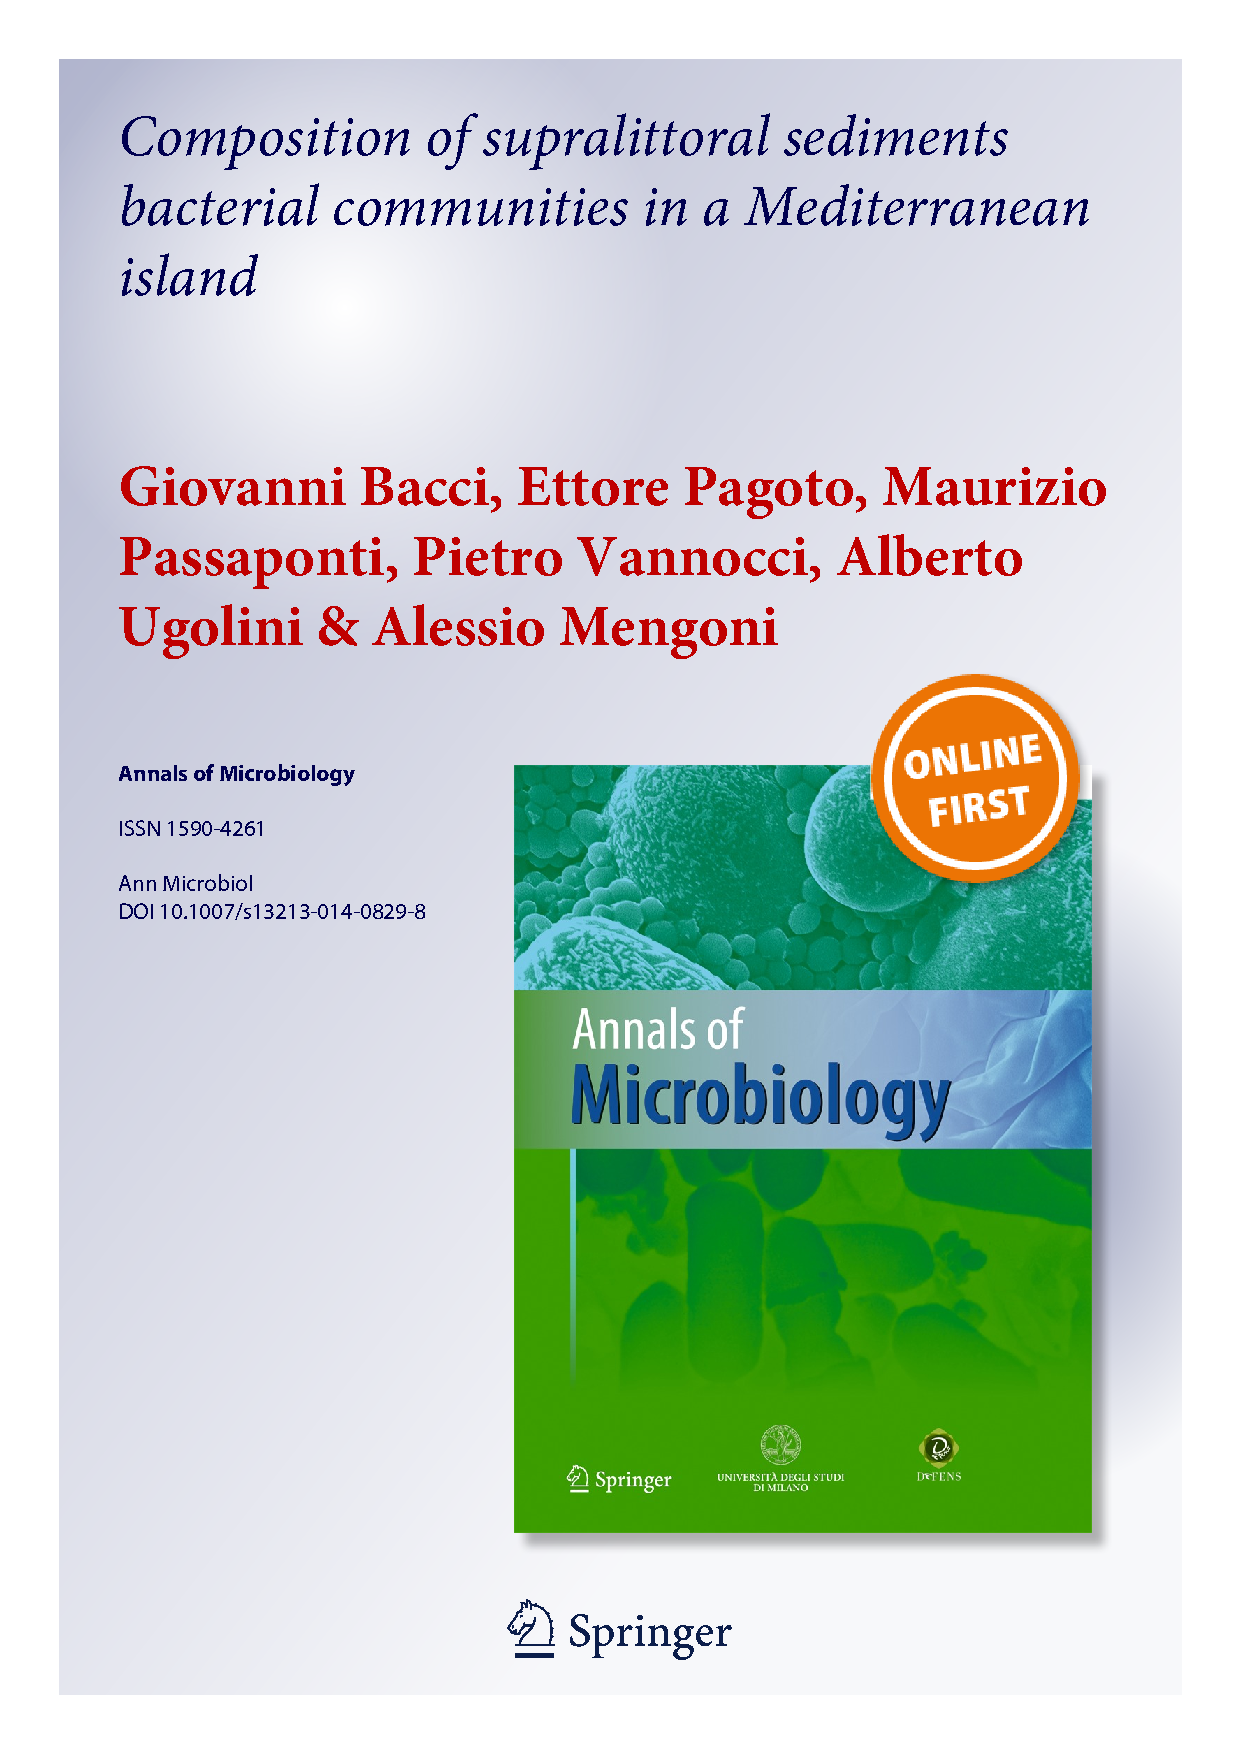
\includepdf[pages=-,offset=10mm 0, scale=0.9]{articles/favignana.pdf}
\newpage

\newpage
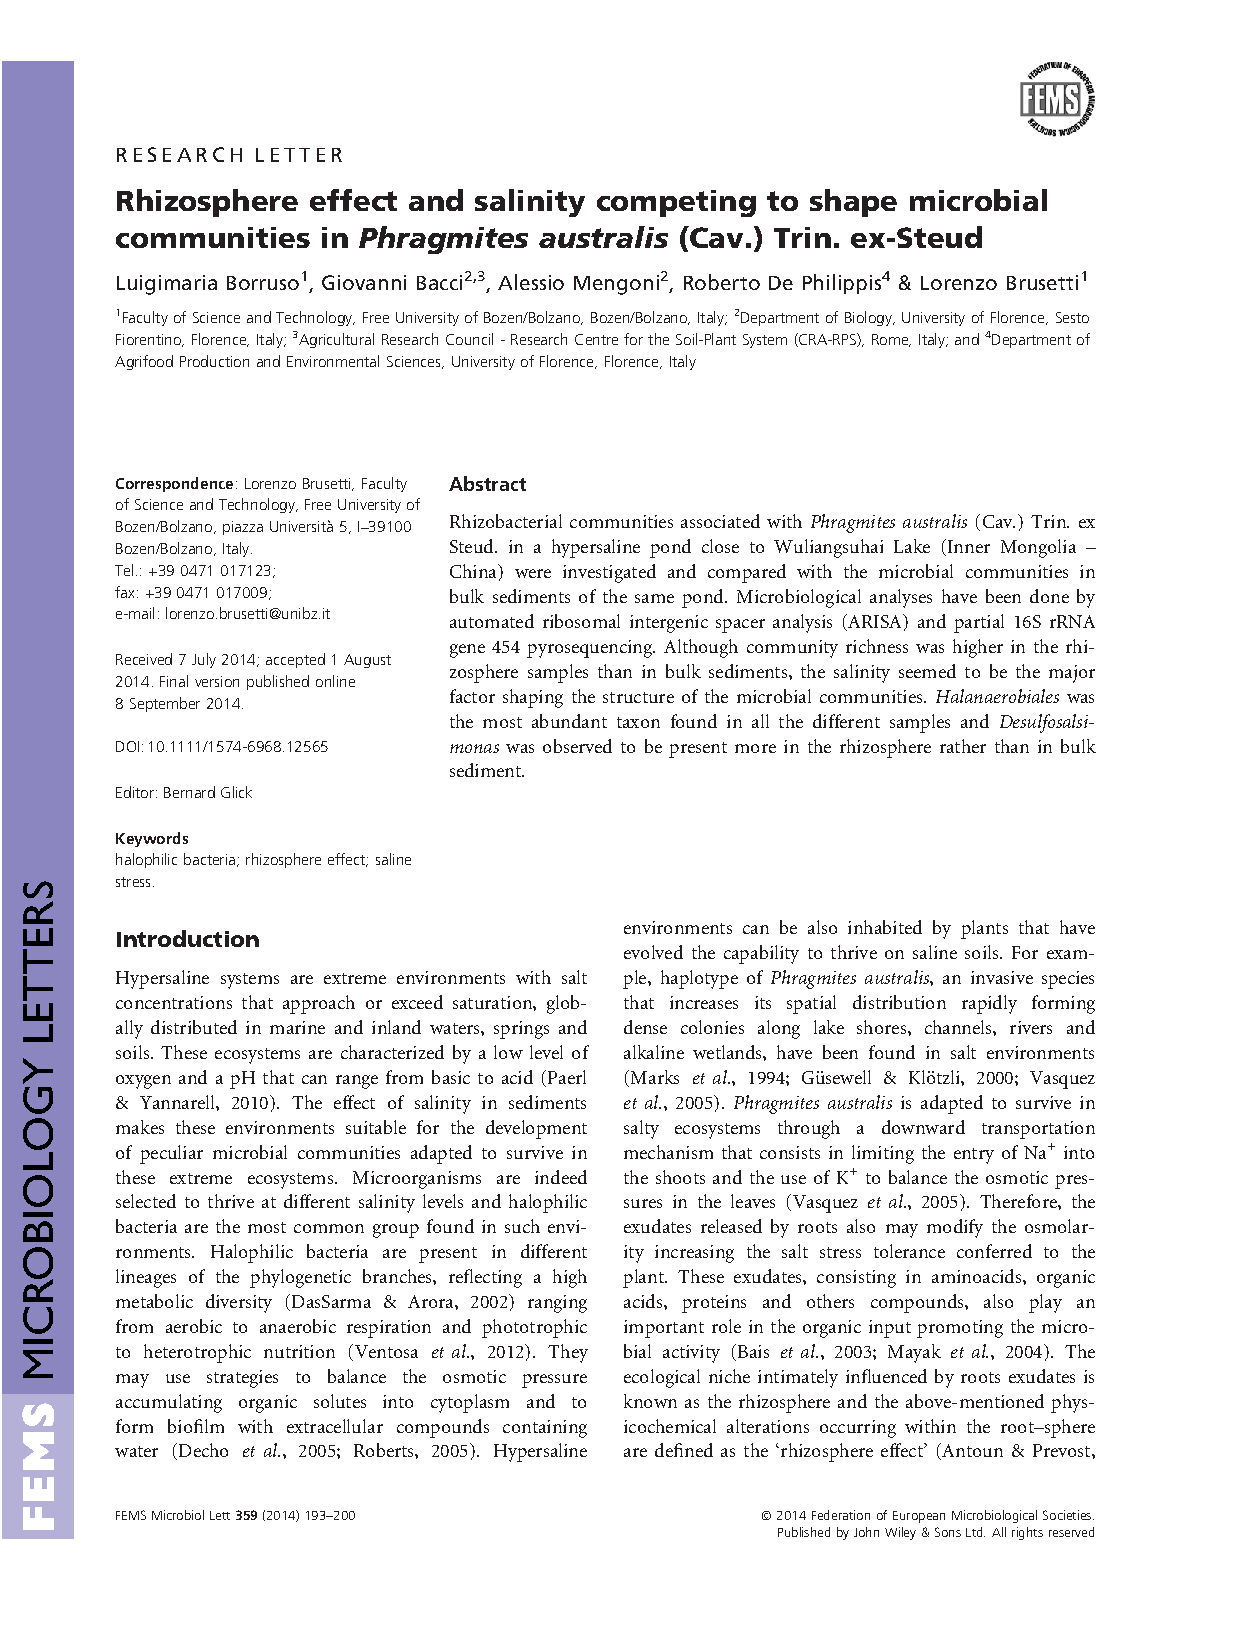
\includepdf[pages=-,offset=10mm 0, scale=0.9]{articles/borrusio.pdf}
\newpage

\newpage
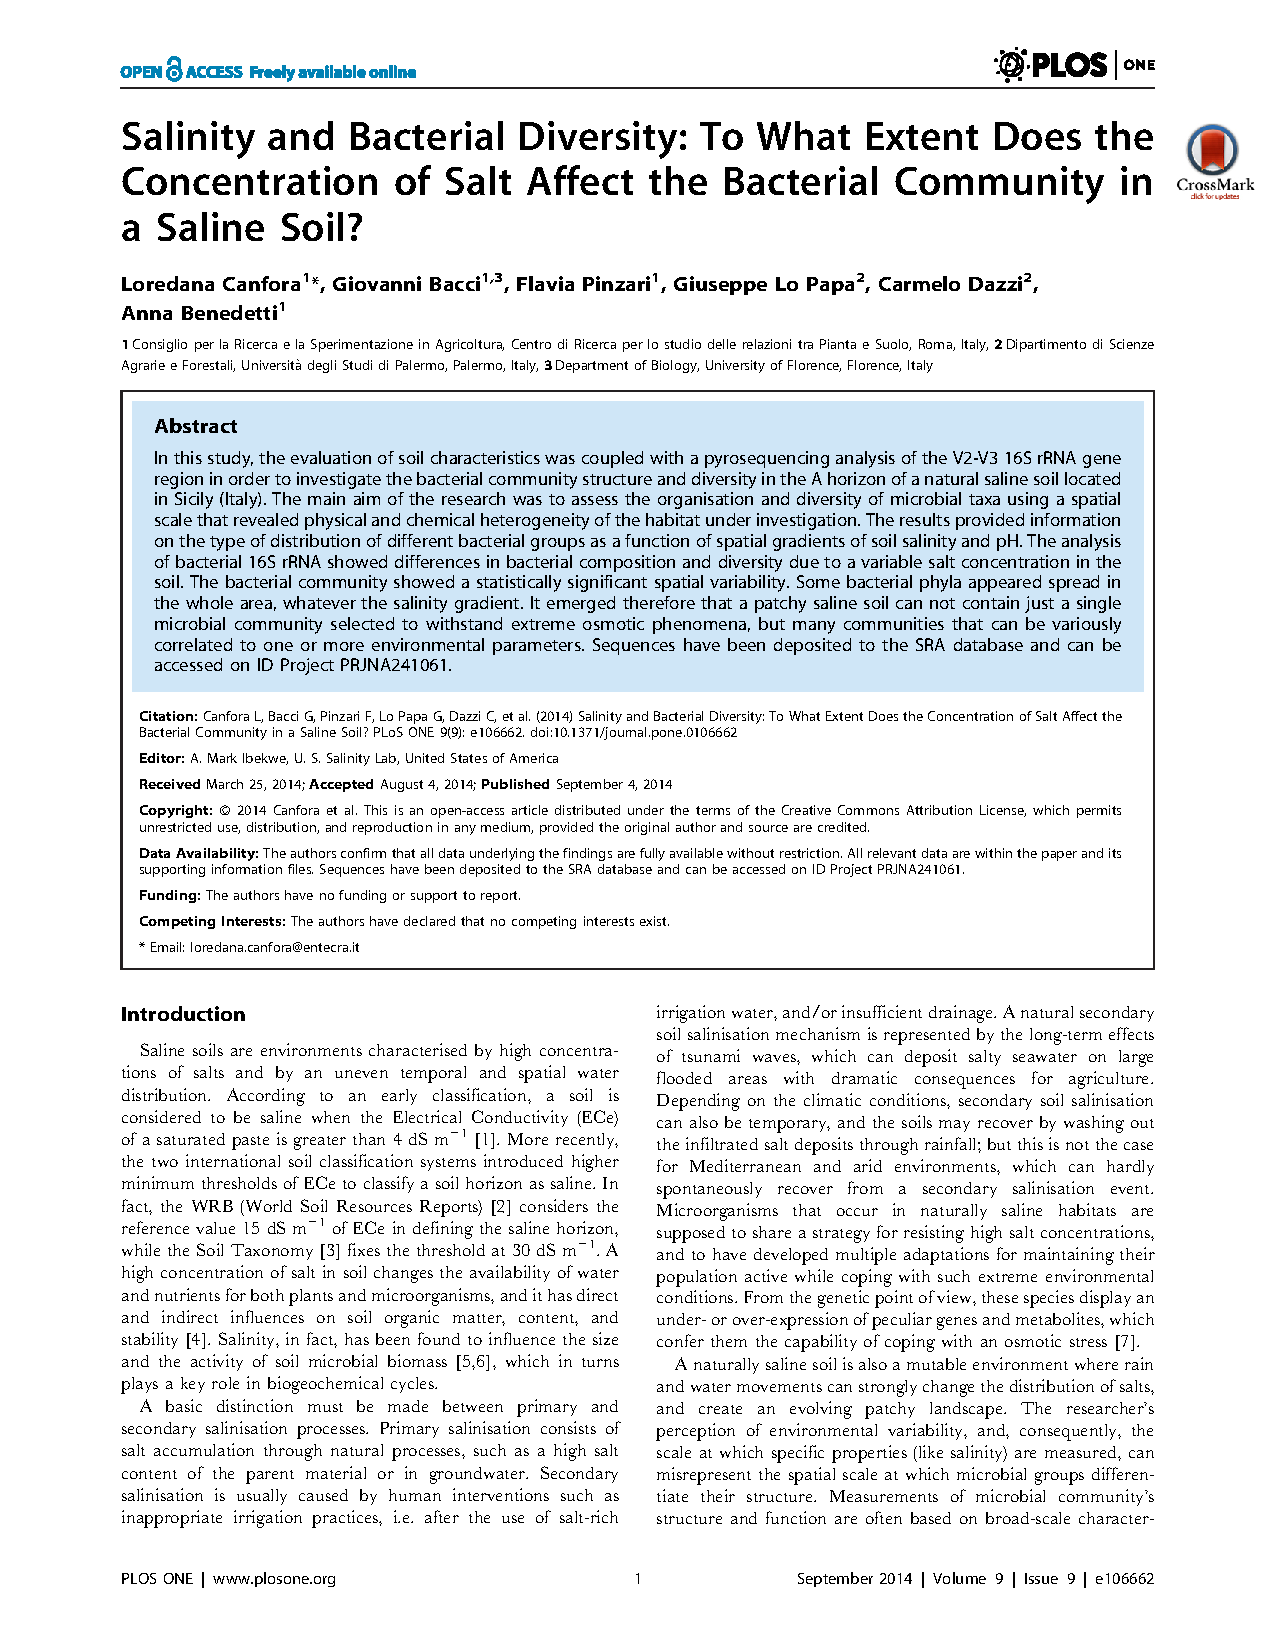
\includepdf[pages=-,offset=10mm 0, scale=0.9]{articles/loredana.pdf}
\newpage


%%-----------
%% Backmatter
%%-----------
\backmatter
\chaptermark{Bibliography}
\renewcommand{\sectionmark}[1]{\markright{#1}}
\bibliographystyle{unsrt}                           %Use alpha codes for references
\sectionmark{Bibliography}
\addcontentsline{toc}{chapter}{Bibliography}        %Force addition of Bibliography to TOC    
\bibliography{References}

\mainmatter
\newthumb
%%%%%%%%%%%%%%%%%%%%%%%%%%%%%%%%%%%%%%%%%%%%%%
\logvartrue
\chapter{Bacteria in agro-environments}
%%%%%%%%%%%%%%%%%%%%%%%%%%%%%%%%%%%%%%%%%%%%%%

\newpage
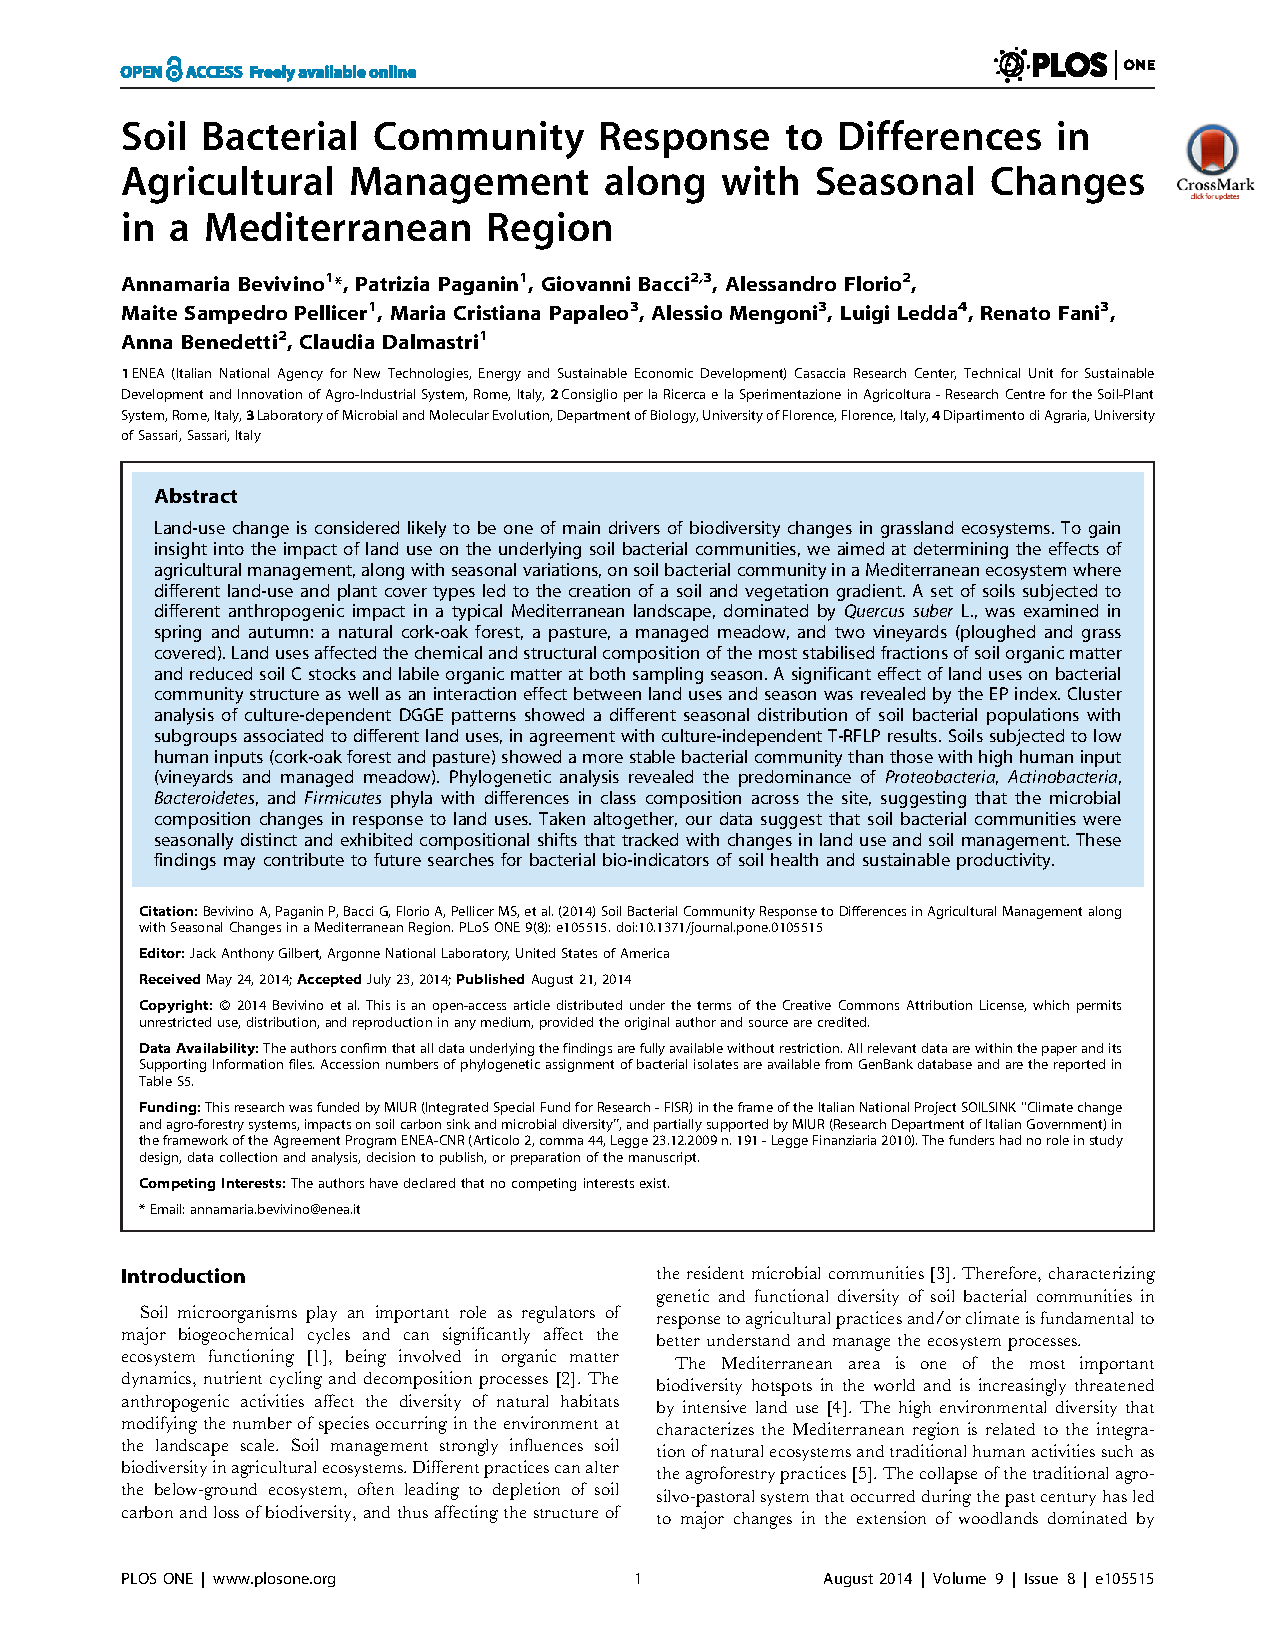
\includepdf[pages=-,offset=10mm 0, scale=0.9]{articles/soil_sink.pdf}
\newpage

%%-----------
%% Backmatter
%%-----------
\backmatter
\chaptermark{Bibliography}
\renewcommand{\sectionmark}[1]{\markright{#1}}
\bibliographystyle{unsrt}                           %Use alpha codes for references
\sectionmark{Bibliography}
\addcontentsline{toc}{chapter}{Bibliography}        %Force addition of Bibliography to TOC    
\bibliography{References}

\mainmatter
\newthumb
%%%%%%%%%%%%%%%%%%%%%%%%%%%%%%%%%%%%%%%%%%%%%%
\logvartrue
\chapter{Bacterial landlord: the microbiome concept}
%%%%%%%%%%%%%%%%%%%%%%%%%%%%%%%%%%%%%%%%%%%%%%
Bacteria have colonized thousands of different environments since the beginning of life on Earth. These environments include all the cavities and tissues, both inside and outside macroscopic organisms such as humans, plants and insects. The interaction between bacteria and their hosts is becoming more and more considered not only as a form of symbiosis but also as an evolution process that involves both the host genome and all the different genomes of the bacterial communities associated with the host itself. The ecological community of commensal, symbiotic, and pathogenic microorganisms that thrive within a host is called ``microbiome''. In recent years, with the development of sequencing techniques able to obtain sequence of DNA directly from environmental sample, the analysis of microbiomes is becoming more and more affordable even by small laboratories. However, due to their great diversity, the comprehension of the bacterial dynamics involved in the host-microbial interaction remains far from our understanding. It is becoming more and more mandatory the development of approaches explicitly developed to cope with meta analyses regarding the host, the bacterial communities and the environment as a whole.\\
These topics have been explained in these papers:
\vspace{-2mm}
\begin{itemize}
\item Mengoni, A., Focardi, A., \textbf{Bacci, G.}, \& Ugolini, A. (2013). High genetic diversity and variability of bacterial communities associated with the sandhopper \textit{Talitrus saltator} (Montagu)(Crustacea, Amphipoda). \textit{Estuarine, Coastal and Shelf Science}, 131, 75-82.
\item \textbf{Bacci, G.}, Abdelrhman, K.F.A., Marras, B., Nistri, A., Schintu, M., Ugolini, A., \& Mengoni, A. The gut microbiota of talitrid amphipods provides insight into the ecology of supralittoral sediments detritivors. Manuscripts submitted to: \textit{FEMS Microbiology Ecology}.
\end{itemize}

\section{High genetic diversity and variability of bacterial communities associated with the sandhopper \textit{Talitrus saltator} (Montagu) (Crustacea, Amphipoda)}
Talitrid amphipods are one of the main components of the damp band of sandy beaches. They play important roles in the flow of energy and nutrients along the sandy beach ecosystem due to both their ability to feed on organic matter and providing nourishment for many species of beetles, fishes, birds and mammals. This work aimed to answer two key basic questions on the ecological interactions of dump band amphipods, using \textit{Talitrus saltator} as model species: $i)$ What is the composition, in taxonomic terms, of the bacterial community associated with single individuals and populations of \textit{T. saltator}? and $ii)$ is there individual or population-specific differentiation of the bacterial community?\\

\newpage
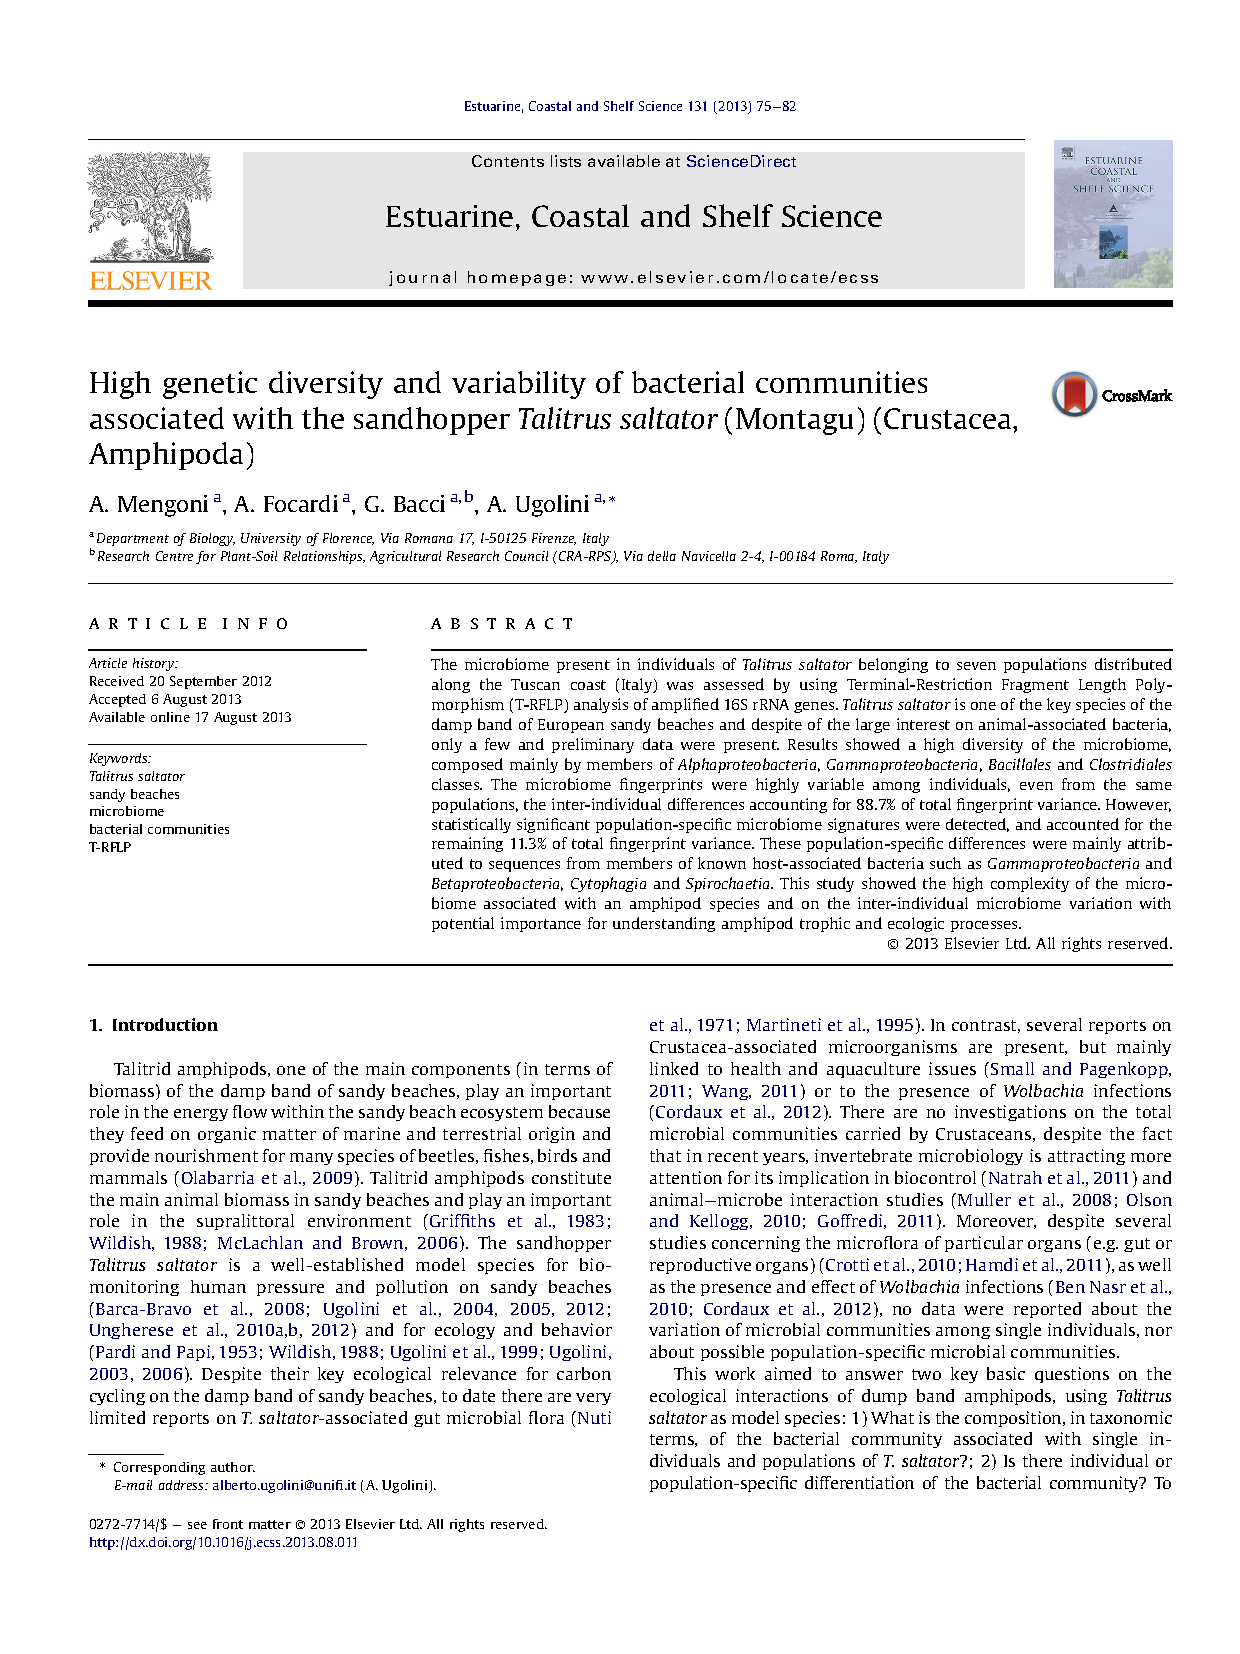
\includepdf[pages=-,offset=10mm 0, scale=0.9]{articles/talitri_1.pdf}
\newpage

%%%%%%%%%%%%%%%%%%%%%%%%%%%%%%%%%%%%%%%%%%%%%%%%%%%%%%%%%%%%%%%%%%%%%%%%%%%%%%%%%%%%%%%%%%%%%%%%%%%%%%%%%%%%%%%%%%%%%%%%%%%%%%%%%%%%%%%%%%%
%%%%%%%%%%%%%%%%%%%%%%%%%%%%%%%%%%%%%%%%%%%%%%%%%%%%%%%%%%%%%%%%%%%%%%%%%%%%%%%%%%%%%%%%%%%%%%%%%%%%%%%%%%%%%%%%%%%%%%%%%%%%%%%%%%%%%%%%%%%

\section{The gut microbiota of talitrid amphipods provides insight into the ecology of supralittoral sediments detritivors}
Talitrid amphipods sandhoppers and beach fleas are colonizers of the supralittoral zone and obtain most of their food from stranded materials, which include detrital marine angiosperms and macroalgae, as well as occasional death animals. Here, we report the characterization of gut microbiota of \textit{Talitrus saltator}, \textit{Talorchestia ugolinii}, \textit{Sardorchestia pelecaniformis}, \textit{Orchestia montagui}, collected in Sardinia (Italy). Microbiota were analyzed by metabarcoding analysis on amplified 16S rRNA V4 region and by quantification of family 48 glycosyl hydrolases genes, which are involved in cellulose degradation. Obtained results indicated the presence of a complex bacterial flora, including several members of \textit{Verrucomicrobia} in four out of the five species. Moreover, different gut microbiota taxonomic assemblages among the selected talitrid species were found. In particular, \textit{O. montagui} (which lives in close contact with \textit{Posidonia} banquette) gut microbiota was found to be the most different with respect to those of the other talitrids, being more abundant in members of \textit{Firmicutes}, \textit{Planctomycetes} and \textit{Actinobacteria}, and containing the highest level of family 48 glycosyl hydrolases genes. We conclude that talitrid amphipods harbour a complex gut microbiota which may be related to the habitat the different species colonizes.\\

\subsection{Introduction}
The microbiome, in particular the gut microbiome, is recognized as an ``extended genotype'' since it encodes a more versatile metabolome than the host \cite{sommer2013gut}. This is particularly relevant for animals which uses lignocellulosic compounds, as preferential food source (e.g. ruminants, termites). In the last years, a number of evidences are accumulating on the role of gut microbiota in determining or correlating with host's ecology in animals (see for instance \cite{becker2009first, basu2010association, bauer2000characterization, behar2008gut, dittmer2012influence}.\\
Talitrid amphipods sandhoppers and beach fleas are crustaceans living in the supralittoral zone and key components of the sandy beach food web \cite{calosi2005physiological, calosi2007physiological, morritt1988osmoregulation, morritt1989ionic, morritt1998physiological, ugolini1995distribution, pardi1986zonal}. Talitrid amphipods obtain most of their food from stranded materials, which include detrital marine angiosperms and macroalgae, as well as occasional death animals \cite{adin2003preferential}. However, among the Mediterranean talitrid taxa, species-specific habitat preferences have been observed. Indeed, some species (as \textit{Talitrus saltator}, \textit{Talorchestia ugolinii}, \textit{Sardorchestia pelecaniformis}) occur in the damp belt of sandy shores, while others (as \textit{Orchestia montagui}) are found under stranded algae and \textit{Posidonia} banquettes, independently from the type of substrate \cite{ugolini1995distribution, pavesi2013genetic}. Finally, for a third group of species (as \textit{Orchestia stephenseni}) the habitat seems to be more heterogeneous, the species being found in the damp of both sand sea shores and pools and lagoons backshore, as well as less within \textit{Posidonia} banquettes and also stranded detritus (e.g. see \cite{pavesi2013genetic, matthaeis2000isolation, lowry2013substrate, deidun2009considerations} and personal observations). Consequently, it is possible to hypothesize a differential food preference and, consequently ,a different taxonomic and functional pattern of gut microbiota among species. However, despite such intriguing question and the key ecological relevance for carbon cycling on the damp band of sandy beaches have talitrid amphipods \cite{griffiths1983kelp}, to date there are very limited reports on beach flea and sandhopper-associated microbial flora \cite{dittmer2012influence, mengoni2013high, nuti1971microrganisms}, and few studies have been performed in general on marine \textit{Crustacea} gut microbiota (e.g. see \cite{harris1993presence, zimmer2001hepatopancreatic, harris1993widespread}).\\
Aim of this work was the analysis of the composition and diversity of the gut microbiota from five different talitrid amphipods species (\textit{Talitrus saltator}, \textit{Talorchestia ugolinii}, \textit{Sardorchestia pelecaniformis}, \textit{Orchestia stephenseni}, \textit{Orchestia montagui}) which may be present in syntopy. In particular, the specific aim is to clarify the presence of gut microbiota signatures which may differentiate the five species, in relation to habitat and food preferences, then providing insight into their different ecology.

\subsection{Materials and Methods\label{par:kalmatmet}}

\subsubsection{Sampling}
Adults and sub-adults talitrids amphipods were collected in September 2013 from eight localities in Sardinia (Italy) (Table~\ref{tab:1kaltal}). For the locality of Giorgino beach, two different sampling points ca. 2 km aparts (named as Giorgino 1 and Giorgino 2) were selected and an additional sampling was also performed on September 2012 for Giorgino 1. In S. Giovanni di Sinis, two species were collected in syntopy (\textit{O. montagui} and \textit{O. stephenseni}). Immediately after collection, guts were excised from animals with sterile forceps and stored in DMSO/EDTA/NaCl preservative solution (20\% DMSO, 0.25 M disodium-EDTA, NaCl to saturation, pH 7.5) \cite{seutin1991preservation, dawson1998field}. Once arrived at the laboratory, samples were then stored at -80{\textdegree}C prior to DNA extraction. Pools composed by gut of ten animals per each species and locality were prepared. When available, for the same locality, two pools were prepared from animals collected at few distance (ca. 10 m), to take into account for possible population-based variation and substrate (e.g. sand and stranded material) heterogeneity. Twelve different pools were then prepared, accounting for a total of 120 single animals.\\
\begin{table}
\centering
\scriptsize
\begin{tabular}{c c c c c}
\hline
Code & Locality & Species & Longitude (E) & Latitude (N)\\
\hline\hline
KA11 & Centro 1{\textdegree} Sassu (Arborea) & {\itshape S. pelecaniformis} & 8{\textdegree}32'48.58{\textquotedbl} E & 39{\textdegree}48'7.08{\textquotedbl} N\\
KA9 & Centro 1{\textdegree} Sassu (Arborea) & {\itshape S. pelecaniformis} & 8{\textdegree}32'48.58{\textquotedbl} E &  39{\textdegree}48'7.08{\textquotedbl} N\\
KA2 & Giorgino 1 & {\itshape T. saltator} & 9{\textdegree}03'61.00{\textquotedbl} E & 39{\textdegree}11'11.41{\textquotedbl} N\\
KA4 & Giorgino 1 & {\itshape T. saltator} & 9{\textdegree}03'61.00{\textquotedbl} E & 39{\textdegree}11'11.41{\textquotedbl} N\\ 
KA5 & Giorgino 2 & {\itshape T. saltator} & 9{\textdegree}02'21.55{\textquotedbl} E & 39{\textdegree}10'26.31{\textquotedbl} N\\
KA12 & Is arenas & {\itshape T. ugolinii} & 8{\textdegree}28'46.35{\textquotedbl} E & 40{\textdegree} 4'13.00{\textquotedbl} N\\ 
KA13 & Is arenas & {\itshape T. ugolinii} & 8{\textdegree}28'46.35{\textquotedbl} E & 40{\textdegree} 4'13.00{\textquotedbl} N\\
KA8 & Maimoni (Cabras) & {\itshape O. montagui} & 8{\textdegree}24'02.36{\textquotedbl} E & 39{\textdegree}54'54.76{\textquotedbl} N\\
KA14 & Piscadeddus & {\itshape O. stephenseni} & 9{\textdegree}28'20.67{\textquotedbl} E & 39{\textdegree} 7'56.73{\textquotedbl} N\\
KA3 & S. Giovanni di Sinis (Cabras) & {\itshape O. montagui} & 8{\textdegree}26'11.03{\textquotedbl} E & 39{\textdegree}52'55.72{\textquotedbl} N\\
KA6 & S. Giovanni di Sinis (Cabras) & {\itshape O. stephenseni} & 8{\textdegree}26'51.42{\textquotedbl} E & 39{\textdegree}53'07.37{\textquotedbl} N\\
KA10 & Sa Rocca Tunda & {\itshape S. pelecaniformis} & 8{\textdegree}25'29.71{\textquotedbl} E &  40{\textdegree} 2'38.01{\textquotedbl} N\\
\hline
\end{tabular}
\caption{Sampled amphipod taxa and sampling locations. The locality with geographical coordinates of sampling point and sampled taxon is indicated.\label{tab:1kaltal}}
\end{table}

\subsubsection{DNA extraction, metabarcoding analysis and detection of cellulase genes}
DNA was extracted from gut tissues by using the QIAamp DNA Investigator Kit (Qiagen), quantified by agarose gel (0.8\% TAE w/v) electrophoresis and by spectrophotometric reading using the \href{http://www.tecan.com/2.2398/Infinite-200-NanoQuant-Specifications}{ Infinite{\textregistered} M200 PRO NanoQuant} (Tecan). From extracted DNA, the bacterial V4 region of 16S rRNA genes was amplified with V4 specific primers \cite{schriml201315th} and sequenced at the IGA Technology Services \href{http://www.igatechnology.com/}{http://www\-.igatech\-nology\-.com/}, Udine, Italy using an Illumina MiSeq apparatus with pair-end sequencing \cite{caporaso2012ultra}. Library preparation and demultiplexing have been performed following Illumina's standard pipeline. Sequence reads have been deposited under  the BioProject ID: PRJNA260027. Total bacterial titres were estimated by Real-Time PCR using a previously reported SybrGreen protocol \cite{bacci2014composition}. The same Real-Time PCR protocol (with annealing temperature decreased to 52{\textdegree}C) was used for detection and Real-Time quantification of glycosyl hydrolase family 48 (GHF48) genes by using GH48F/GH48R primer pair \cite{izquierdo2010diversity}. Standard curves for 16S rRNA and GHF48 have been prepared with serial dilutions of genomic DNA of \textit{Streptomyces coelicolor} A3 (2), which contains a putative GHF48 gene (SCO5456).\\

\subsubsection{Raw data processing}
Raw sequence data generated from Illumina sequencing were processed following several steps. First of all, sequences were quality trimmed with StreamingTrim 1.0 \cite{bacci2014streamingtrim}. Quality trimmed sequences were assembled and subjected to another quality control step with PANDAseq \cite{masella2012pandaseq}. Processed sequences were then subjected to the UPARSE pipeline \cite{edgar2013uparse}, in order to remove chimeric sequences (both in de novo and in reference mode) and to cluster them into Operational Taxonomic Units (OTUs). An identity threshold of 97\% has been used \cite{konstantinidis2007prokaryotic}. Representative sequences obtained from the UPARSE clustering were taxonomically classified using the SINA standalone classifier using the ``Ref NR 99'' as reference database \cite{pruesse2012sina}. After taxonomic classification we removed from our dataset all OTUs not assigned at least at Bacteria domain.\\

\subsubsection{Biodiversity indexes analysis and statistical analysis}
Rarefaction curves have been generated using the OTU assignments. Sample assignments have then be rarefied using a number of random subsamples equal to the number of assignments of the smaller sample Shannon, Richness and Evenness indexes were calculated on the rarefied samples; In order to investigate the presence of species-specific patterns in the metabarcoding data of gut microbiota of the talitrid amphipds OTU abundances were then used to perform a Canonical Correlation Analysis. Real-Time PCR data were statistically analyzed by one- ay ANOVA. All statistical analyses were performed with the R software with the following packages: vegan \cite{dixon2003vegan, oksanen2007vegan}; igraph \cite{csardi2006igraph} and ggplot2 \cite{ginestet2011ggplot2}.\\

\subsubsection{Network construction and clustering}
In order to generate a OTUs network displaying patterns of correlation between each OTU, we calculated Spearman's correlations between all OTUs in our dataset, regardless of the sample of origin. Each OTU has been considered as a vertex inside the network and an edge between two OTUs has been created only if the Spearman's correlation coefficient between those OTUs was statistically significant (p {\textless} 0.05) and r {\textgreater} 0.5. In this way we generate an edge linking two OTUs only when there is a statistically significant and high degree of correlation between the two OTUs. In order to inspect the OTU distribution in the generated network the Markov Cluster Algorithm (MCL) was used \cite{van2000graph}. This method uses only one parameter in order to choose the number of cluster to generate; this parameter is called ``inflation values'' and it can range between 1.2 and 5.0 as reported by the author of the algorithm. In order to find the ``inflation value'' (IF) resulting in an informative number of clusters we used the ``intracluster clustering coefficient'' (ICCC) method \cite{lima2008reticulate}). Thus, we generated 39 different clusters using all IF values between 1.2 and 5.0 increasing the IF value by 0.1 each time and calculating the ICCC value for each clustering. Finally, the IF value that maximize the ICCC was 1.4 with the generation of 5 clusters. A representation of the generated network was drawn using Gephi \cite{bastian2009gephi} with the ``Force Field layout''; nodes were colored based on the cluster attribution.\\

\subsection{Results and Discussion}

\subsubsection{Representativeness and diversity of gut microbiota}
The metabarcoding analysis of 16S rRNA genes from the twelve gut DNA samples, representing five different talitrid species resulted in a relatively good coverage of bacterial diversity, with almost all samples reaching saturation or near saturation values (Figure~\ref{fig:1talkal}). A total number of 7606010 (15212020 paired-end) reads was obtained with 410864 to 846775 reads per sample. After clustering at 97\% identity a total of 1004 OTUs were identified in the twelve samples (Table SM1).\\
\begin{figure}[!tb]
	\centering
	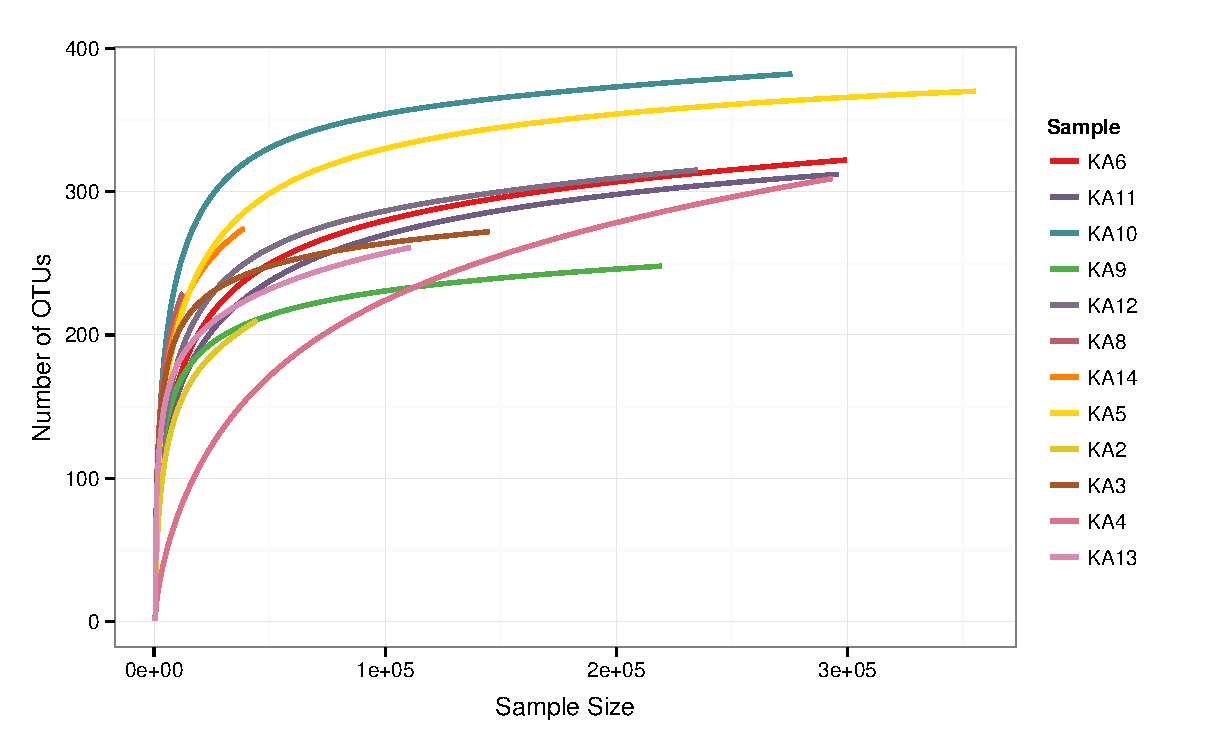
\includegraphics[width=1\textwidth]{./figures/Chapter_6/Figure_1_talkaled.eps}
  	\caption{Representativeness of sampled gut microbiota. The number of Operating Taxonomic Units (OTUs) as a function of
the number of sampled sequences is reported. The sequences were sampled with a step size of 100 sequences in order to
generate smooth curves. The asymptotic trends of curves indicate that a reasonable number of reads has been generated
in order to inspect the diversity of each sample. The different end values indicates variable numbers of clustered
sequences per sample.\label{fig:1talkal}}
\end{figure}
The analysis of community diversity for each samples (Table~\ref{tab:2kaltal}) showed  the lowest values for all three indices (Richness, Shannon and Evenness) for KA6 sample (\textit{O. montagui}), while the highest values were reached by the other \textit{O. montagui} sample (KA3), for Shannon and Evenness and by \textit{S. pelecaniformis} (KA10) for Richness. However, no statistically significant differences were found in relation to both talitrid species and locality of sampling (Table SM2).\\
\begin{table}
\centering
\scriptsize
\begin{tabular}{ c c c c c c }
\hline
Species & Locality & code & Richness & Shannon H & Evenness\\
\hline\hline
{\itshape O. montagui} & S. Giovanni di Sinis (Cabras) & KA3 & 322 & 3.995 & 0.692\\
{\itshape O. montagui} & Maimoni (Cabras) & KA8 & 229 & 0.497 & 0.091\\
{\itshape O. stephenseni} & Piscadeddus & KA14 & 274 & 0.931 & 0.166\\
{\itshape O. stephenseni} & S. Giovanni di Sinis (Cabras) & KA6 & 366 & 2.846 & 0.482\\
{\itshape S. pelecaniformis} & Centro 1{\textdegree} Sassu (Arborea) & KA11 & 294 & 3.473 & 0.611\\
{\itshape S. pelecaniformis} & Centro 1{\textdegree} Sassu (Arborea) & KA9 & 338 & 2.207 & 0.379\\
{\itshape S. pelecaniformis} & Sa Rocca Tunda & KA10 & 430 & 3.957 & 0.653\\
{\itshape T. saltator} & Giorgino & KA2 & 413 & 3.485 & 0.579\\
{\itshape T. saltator} & Giorgino & KA4 & 205 & 0.783 & 0.147\\
{\itshape T. saltator} & Giorgino & KA5 & 311 & 1.790 & 0.312\\
{\itshape T. ugolinii} & Is arenas & KA & 372 & 3.120 & 0.527\\
{\itshape T. ugolinii} & Is arenas & KA12 & 287 & 2.564 & 0.453\\
\hline
\end{tabular}
\caption{Diversity indices of microbiota. Diversity indices of gut microbiota in the twelve metabarcoding samples.\label{tab:2kaltal}}
\end{table}

\subsubsection{Species-specific signatures of gut microbiota}
Numerous evidences indicate that animals co-evolve with their gut microbiota \cite{ley2008worlds}. Consequently, species-specific patterns in the metabarcoding data of gut microbiota of the talitrids amphipds were inspected. Figure~\ref{fig:2talkal} reports the CCA  results, which indicate the presence of clearly separate clusters for the five species under analysis (\textit{O. montagui}, \textit{S. pelecaniformis}, \textit{T. saltator}, \textit{T. ugolinii}, \textit{O. stephensenii}), then supporting the hypothesis that amphipod digestive tracts host species-specific bacterial communities, which may be related to both the phylogeny and to potential dietary differences among the amphipod species, as exemplified in vertebrates \cite{ley2008worlds}.\\
\begin{figure}[!tb]
	\centering
	\includegraphics[width=0.7\textwidth]{./figures/Chapter_6/Figure_2_talkaled.eps}
  	\caption{Species-specific signatures of gut microbial community composition. Canonical Correlation Analysis (CCA) based
on OTU assignments to the bacterial taxonomy.\label{fig:2talkal}}
\end{figure}
As recently proposed for soil bacterial communities \cite{barberan2011using}, network analysis of significant taxon co-occurrence patterns could be useful to decipher the structure of complex microbial communities. Several works have shown recently that network analysis of co-occurrence may allow to define community patterns in several environments (for examples \cite{berry2014deciphering, boutin2014inter, williams2014demonstrating, geng2014co} see). Consequently, to further inspect the species-specific signatures of our amphipod gut microbiota a network analysis was conducted on Pearson's correlations among OTUs. This analysis, coupled with a k-means clustering, highlighted the presence of five taxonomically differentiated groups (clusters) of co-occurring OTUs (Figure~\ref{fig:3talkal}), in particular concerning \textit{Proteobacteria}, \textit{Actinobacteria} and \textit{Firmicutes}. Such clusters showed different representation in the five amphipod taxa (Figure SM1). In particular, cluster 4 was practically absent in \textit{S. pelecaniformis}, while the other clusters showed both a high variability among species, as well as among samples within the same species.\\
\begin{figure}[!tb]
	\centering
	\includegraphics[width=0.9\textwidth]{./figures/Chapter_6/Figure_3_talkaled.eps}
  	\caption{Network-based signatures of species-specific microbiota composition. Correlation network of OTU assignments. Each connection stands for a high degree of correlation between the two OTUs connected (Spearman's correlation r {\textgreater} 0.6 and p-value {\textless} 0.05). The size of each node in the network is proportional to its degree (number of connection of the node). The color of each node corresponds to a cluster obtained with the MCL algorithm with an ``inflation value'' equal to 1.4 (see section~\ref{par:kalmatmet}). Clusters have been defined after a k-means clustering.\label{fig:3talkal}}
\end{figure}

\subsubsection{Taxonomic differences in gut microbiota among talitrid species}
To evaluate which bacterial taxa mostly contribute to the interspecific differences of gut microbiota, OTUs were then assigned to bacterial phylogeny (Table SM3). Figure~\ref{fig:4talkal} shows the overall representation of taxonomic composition of gut microbiota, which highlight similar patterns, among all samples, with differences both within the same species, and among species. In particular, it could be worth of mentioning that \textit{Verrucomicrobia} were present in four out of five species (absent from all \textit{S. pelecaniformis} samples), as well as the group \textit{Deinococcus/Thermus} absent in both \textit{Orchestia} species. \textit{Verrucomicrobia} are particularly intriguing since this phylum, closely related to \textit{Planctomycetes} and \textit{Chlamydiae}, is considered to be particularly frequent in nonhost-assocaited environments, as soil and waters \cite{buckley2001environmental,freitas2012global}. \textit{Verrucomicrobia} have been suspected to contribute to energy generation from fermentable substrates in the human gut \cite{arumugam2011enterotypes} and \textit{Verrucomicrobia} have been found as particularly abundant after antibiotic treatment \cite{dubourg2013high}. We cannot consequently exclude that \textit{Verrucomicrobia} (present in all but \textit{S. pelecaniformis} samples) may have a role in some hypothetical differential nutrient assimilation in those talitrid species and in differential resilience toward environmental disturbance, which is frequent in sandy beaches \cite{defeo2009threats, ugolini2012sandhoppers, ugolini2005heavy, ugolini2008amphipod, ungherese2010relationship, moffett1998impact}.\\
\begin{figure}[!tb]
	\centering
	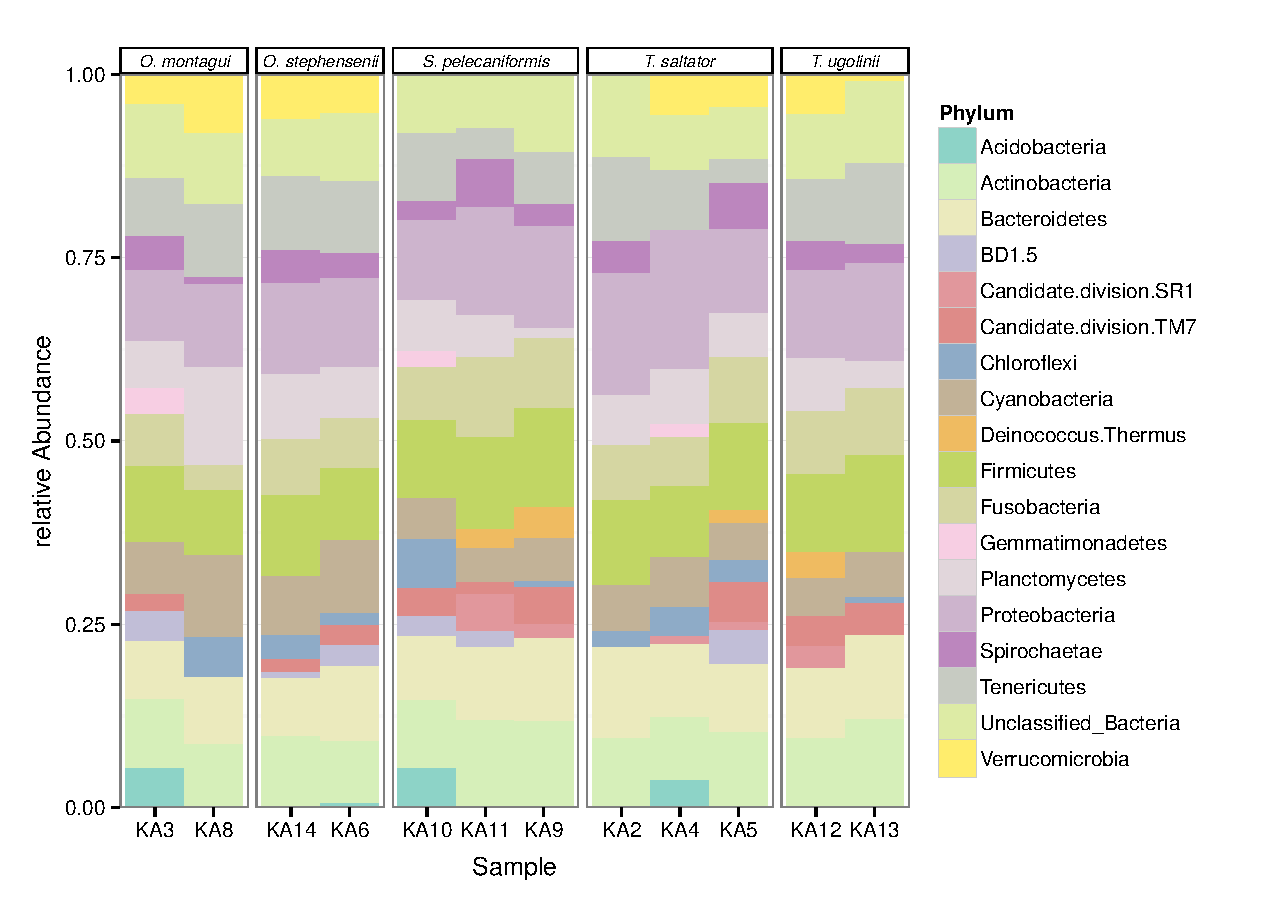
\includegraphics[width=1\textwidth]{./figures/Chapter_6/Figure_4_talkaled.eps}
  	\caption{Taxonomic composition of gut microbiota. Relative abundances barplot showing the relative abundance of bacterial phyla in each gut sample.\label{fig:4talkal}}
\end{figure}
To more in deep clarify the relative contribution of each phylum in species-specific gut microbiota signatures, a similarity percentage (simper) analysis was conducted (Table~\ref{tab:3kaltal}, Table SM3). In general, the phyla mostly contributing to differences between talitrid species are the most abundant, as \textit{Proteobacteria} (5.5\%-9.1\%), \textit{Firmicutes }(5.2\%-9.0\%), \textit{Bacteriodetes} (5.0\%-6.3\%), and \textit{Actinobacteria} (4.9\%-8.6\%). Interestingly, \textit{O. montagui}, which inhabits within the Posidonia banquettes  and macroalgae mat, shows the highest percentage of variance for \textit{Planctomycetes} in all pairwise comparisons, as well as among the highest percentage of variance for \textit{Firmicutes} also. \textit{Planctomycetes} have been found to densely populate the alkaline part of the hindgut of soil-feeding termites (\textit{Cubitermes} spp.) \cite{kohler2008novel} and to strongly vary with diet in humans \cite{cayrou2013molecular}. Moreover, \textit{Planctomycetes} constitute a large part of bacterial biofilms found on macroalgae \cite{lage2014planctomycetes}. The relative importance of \textit{Firmicutes} and \textit{Planctomycetes} in differentiating \textit{O. montagui }gut\textit{ }microbiota from those of the other talitrid species, may be due to the habitat of this species, possibly linked to the potential higher cellulose content of its diet. Of course confirmatory experiments under controlled conditions are needed to better evaluate the relative contribution of diet with respect to species in determining the specific of \textit{O. montagui }gut microbiota, especially in comparison with \textit{O. stephenseni}, which has been found in syntopy in the S. Giovanni di Sinis site (KA3 and KA6, Table~\ref{tab:1kaltal}).\\
\begin{landscape}
\begin{table}
\centering
\tiny
\begin{tabular}{ p{0.04\textwidth} p{0.04\textwidth} p{0.04\textwidth} p{0.04\textwidth} p{0.04\textwidth} p{0.04\textwidth} p{0.04\textwidth} p{0.04\textwidth} p{0.04\textwidth} p{0.04\textwidth} p{0.04\textwidth} p{0.04\textwidth} p{0.04\textwidth} p{0.04\textwidth} p{0.04\textwidth} p{0.04\textwidth} p{0.04\textwidth} p{0.04\textwidth} p{0.04\textwidth}}
\hline
 & Acido\-bacte\-ria & Actino\-bacte\-ria & Bacte\-roide\-tes & BD1.5 & SR1 & TM7 & Chlo\-rofl\-exi & Cyano\-bacte\-ria & Denico\-ccus/Ther\-mus & Fir\-micu\-tes & Fuso\-bacte\-ria & Placto\-myce\-tes & Proteo\-bacte\-ria & Spir\-ocha\-ete & Tene\-ricu\-tes & Unclas\-si\-fied & Verruco\-micro\-bia & Gemmati\-monade\-tes\\
\hline\hline
Os vs Sp & 0.65\% & 5.94\% & 5.54\% & 0.11\% & 0.11\% & 0.11\% & 0.66\% & 0.64\% & 0.11\% & 5.86\% & 0.36\% & 2.41\% & 7.81\% & 0.20\% & 0.34\% & 0.33\% & 0.53\% & NA\\
Os vs Tu & NA & 5.58\% & 4.99\% & 0.13\% & NA & 0.13\% & 0.13\% & 0.89\% & 0.12\% & 5.23\% & 0.54\% & 2.70\% & 6.82\% & 0.16\% & 0.40\% & 0.40\% & 0.69\% & NA\\
Os vs Om & 0.36\% & 6.50\% & 5.75\% & 0.17\% & NA & NA & NA & 1.16\% & NA & 8.68\% & 0.70\% & 6.10\% & 7.03\% & 0.21\% & 0.31\% & 0.51\% & 0.70\% & NA\\
Os vs Ts &NA & 7.73\% & 5.69\% & 0.15\% & NA & 0.15\% & 0.30\% & 0.59\% & NA & 7.02\% & 0.74\% & 2.80\% & 9.09\% & 0.26\% & 0.43\% & 0.42\% & 0.65\% & NA\\
Sp vs Tu & 0.67\% & 4.88\% & 5.07\% & 0.10\% & 0.10\% & NA & 0.70\% & 0.77\% & 0.09\% & 5.45\% & 0.32\% & 1.75\% & 6.20\% & 0.29\% & 0.17\% & 0.35\% & 0.23\% & NA\\
Sp vs Om & 0.57\% & 7.23\% & 6.34\% & 0.16\% & 0.16\% & 0.15\% & 0.31\% & 1.06\% & 0.15\% & 9.02\% & 1.00\% & 5.14\% & 6.94\% & 0.35\% & 0.35\% & 0.43\% & 0.34\% & 0.12\%\\
Sp vs Ts & 0.27\% & 8.24\% & 5.94\% & 0.15\% & 0.15\% & 0.14\% & 0.86\% & 0.56\% & 0.14\% & 8.23\% & 0.80\% & 1.25\% & 8.07\% & 0.45\% & 0.29\% & 0.44\% & 0.07\% & NA\\
Tu vs Om & 0.29\% & 7.88\% & 5.78\% & 0.17\% & NA & 0.17\% & NA & 1.14\% & NA & 8.89\% & 0.95\% & 5.66\% & 5.73\% & 0.10\% & 0.31\% & 0.51\% & 0.40\% & NA\\
Tu vs Ts & NA & 8.58\% & 5.88\% & NA & NA & 0.15\% & 0.15\% & 0.76\% & 0.15\% & 8.23\% & 0.84\% & 1.61\% & 7.21\% & 0.17\% & 0.34\% & 0.50\% & 0.25\% & NA\\
Om vs Ts & 0.65\% & 7.16\% & 5.98\% & 0.18\% & NA & 0.18\% & 0.52\% & 0.86\% & NA & 9.03\% & 0.87\% & 6.23\% & 7.63\% & 0.31\% & 0.41\% & 0.51\% & 0.59\% & 0.14\%\\
\hline
\end{tabular}
\caption{Species-specificity of bacterial phyla. Results of simper analysis. The percentage of variance attributed to each phylum in pairwise comparisons of talitrid species is reported. In bold pairwise comparison with \textit{O. montagui}. Om,, \textit{O. montagui}; Sp, \textit{S. pelecaniformis}; Ts, \textit{T. saltator}; Tu, \textit{T. ugolinii}; Os, \textit{O. stephenseni}.\label{tab:3kaltal}}
\end{table}
\end{landscape}

\subsubsection{Cellulolytic bacteria may contribute to \textit{O. montagui} gut microbiota difference}
From the analysis of taxonomic pairwise differences in gut microbiota (Table~\ref{tab:3kaltal}), it emerged that among the most important bacterial phyla, those of \textit{Firmicutes} and \textit{Planctomycetes} were particularly related to possible dietary/habitat differences between \textit{O. montagui} and the other talitrids. Both \textit{Firmicutes} and \textit{Planctomycetes} includes cellulose-degrading strains \cite{kulichevskaya2007schlesneria, schwarz2001cellulosome}. Additionally, a large proportion of \textit{Actinobacteria}(Figure~\ref{fig:4talkal}), which are well known to include many cellulolytic strains \cite{ljungdahl1985ecology}, has been found in all talitrid species. These evidence raised the question if the proportion of cellulosolytic bacteria with respect to the total bacterial load of the gut, may indeed be different between amphipod talitrids. However, from the molecular point of view, it is difficult to have a global overview of all genes encoding cellulases in a sample. Cellulase systems are in fact complex assemblages of multifunctional glycosyl hydrolases \cite{schwarz2001cellulosome}. Many families of glycosyl hydrolases have been found \cite{lynd2002microbial}, hampering the possibility to develop universal primers for PCR detection of all known cellulases. However, family 48 glycosyl hydrolases are well represented in many model cellulolytic clostridia and actinobacteria \cite{lynd2002microbial, beloqui2010diversity}.Primer pairs have been developed for 48 glycosyl hydrolases genes identification and quantification in environmental samples \cite{izquierdo2010diversity,pereyra2010detection}, in particular for clostridia and actinobacteria \cite{izquierdo2010diversity}. Since in our study a considerable fraction of recovered taxa fall within both \textit{Firmicutes} and \textit{Actinobacteria} (approx. 25\% of reads) we decided to investigate the presence of family 48 glycosyl hydrolases genes in amphipod gut microbiota. Results of the qPCR analysis are reported in Table 4. Interestingly, \textit{O. montagui} gut samples contained a higher ratio of GHF48 genes/16S rRNA genes (considered as estimators of the total number of bacterial cells) with respect to the other talitrid species, suggesting that indeed the different microbiota present in \textit{O. montagui} gut may be partly related to a higher prevalence of feeding on cellulose-rich substrates by this species.\\

\subsection{Conclusions}
Talitrid amphipods inhabiting supralittoral environment obtain most of their food from stranded materials, which include debris of various origin, as death animal organisms, macroalgae and plants (as land plants and \textit{P. oceanica} in the Mediterranean sea) \cite{adin2003preferential, colombini2011food}. In particular, due to the presence of low digestible components including lignocellulosic compounds in macroalgae and plants, we can hypothesize that a cellulosolytic bacterial flora in the digestive tract of talitrids could contribute in cellulose degradation. Indeed, previous authors \cite{nuti1971microrganisms, olabarria2009intraspecific} reported the presence of cellulose-degrading bacterial strain in the gut of talitrid amphipods, supporting the hypothesis of the involvement of gut microbiota in carbon source assimilation by such species. Here, we indicate that among the sampled species, which colonizes different microhabitats, \textit{O. montagui} (which is found within \textit{Posidonia} and macroalgae banquettes) harbors a different gut microbiota with respect to the other species. The \textit{O. montagui} gut microbiota includes more taxa known to be involved in cellulose degradation and an analysis of family 48 glycosyl hydrolases (one of the cellulase genes) indicated that indeed \textit{O. montagui} gut harbor a higher number of cellulose-degrading cells than the other talitrids. We conclude that the different ecological behavior of \textit{O. montagui} (a colonizer of \textit{Posidonia} banquettes) could be related also to a different taxonomic and functional composition of its gut microbiota. We cannot however, a priori exclude that a contribution of host encoded glycosyl hydrolases to food digestion could be present in \textit{O. montagui} and in the other talitrid amphipods, as demonstrated for the marine isopod \textit{Limnoria quadripunctata} \cite{king2010molecular}. Moreover, since \textit{O. montagui} shows a low population structure, probably due to its high capacity of dispersion \cite{matthaeis2000isolation}, it remains to explain the quite relevant differences between the two pools of specimens of \textit{O. montagui} gut microbiota investigated here, with respect to those of the other species, as \textit{O. stephenseni}. Consequently, further investigation will be needed to elucidate the differences between \textit{O. montagui} and \textit{O. stephenseni} gut microbiomes and  the relative influence of diet on gut microbial communities.\\

\subsection{Acknowledgments}
We are grateful to the directions of the Protected Marine Areas ``Penisola del Sinis e Mal di Ventre'' and ``Capo Carbonara'' for authorization to samplings and logistic support and to Marco Confalone for technical assistance during DNA extraction. We are also indebted with Dr. D. Bellan--Santini (Centre d'Oc\'{e}anologie de Marseille-DIMAR) for her help in the identification of some amphipod specimens. This work was supported by a grant from Regione Autonoma della Sardegna (L.R. 7/8/2007, N.7), code CRP-28345 and by a grant to KFAA from the Libyan Government. GB is supported by a PhD fellowships from CRA-RPS.\\

%%-----------
%% Backmatter
%%-----------
\backmatter
\chaptermark{Bibliography}
\renewcommand{\sectionmark}[1]{\markright{#1}}
\bibliographystyle{unsrt}                           %Use alpha codes for references
\sectionmark{Bibliography}
\addcontentsline{toc}{chapter}{Bibliography}        %Force addition of Bibliography to TOC    
\bibliography{References}

\mainmatter
\newthumb
%%%%%%%%%%%%%%%%%%%%%%%%%%%%%%%%%%%%%%%%%%%%%%
\logvartrue
\chapter{Microbiome in human disease}
%%%%%%%%%%%%%%%%%%%%%%%%%%%%%%%%%%%%%%%%%%%%%%
The interest in the role of the microbiome in human health has increased over the past decade, in conjunction with the development of new technologies for exploring complex microbial communities. The large-scale dynamics of the microbiome can be described by many of the tools and observations used in several studies of population ecology. Deciphering the human microbiome and its taxonomic signatures can also be used to deeply understand the properties of the microbial communities inside the human body and their correlation with human diseases. Therefore, both the microbiome and metagenome probably have important functions in health and disease and their exploration is a new challenge in human genetics.\\
These topics have been discussed in the following papers:
\vspace{-2mm}
\begin{itemize}
\item Paganin, P., Fiscarelli, E.V., Tuccio, V., Chiancianesi, M., \textbf{Bacci, G.}, Morelli, P., Dolce, D., Dalmastri, C., De Alessandri, A., Lucidi, V., Taccetti, G., Mengoni, A., \& Bevivino, A. Changes in Cystic Fibrosis Airway Microbial Community Associated with a Severe Decline in Lung Function. Manuscripts submitted to: \textit{PloS one}.
\item \textbf{Bacci, G.}, Paganin, P., Lopez, L., Vanni, C., Dalmastri, C., Cantale, C., Daddiego, L., Perrotta, G., Taccetti, G., De Alessandri, A., Fiscarelli, E.E., Lucidi, V., Bevivino, A., \& Mengoni, A. Taxonomic signatures of CF airway microbiota distinguish between stable and severe declining patients. Manuscripts to be  submitted to: \textit{Proceedings of the National Academy of Sciences}
\end{itemize}

\section[Changes in Cystic Fibrosis Airway Microbial Community Associated with a Severe Decline in Lung Function]{Changes in Cystic Fibrosis Airway Microbial Community Associated with a Severe Decline in Lung Function%
\sectionmark{Lung microbiota of CF patients}}
\sectionmark{Lung microbiota of CF patients}

Cystic fibrosis (CF) is a genetic disease resulting in chronic polymicrobial infections of the airways and progressive decline in lung function. To gain insight into the underlying causes of severe lung diseases, we aimed at comparing the airway microbiota detected in sputum of CF patients with stable lung function (S) versus those with a substantial decline in lung function (SD). Microbiota composition was investigated by using culture-based and culture-independent methods, and by performing multivariate and statistical analyses. Culture-based methods identified some microbial species associated with a worse lung function, i.e. \textit{Pseudomonas aeruginosa}, \textit{Rothia mucilaginosa}, \textit{Streptococcus pneumoniae }and \textit{Candida albicans}, but only the presence of \textit{S. pneumoniae }and \textit{R. mucilaginosa }was found to be associated with increased severe decline in forced expiratory volume in 1 second (FEV\textsubscript{1}). Terminal-Restriction Fragment Length Polymorphism (T-RFLP) analysis revealed a higher bacterial diversity than that detected by culture-based methods. Molecular signatures with statistically significant odds ratio for SD status were detected, and classified as \textit{Pseudomonas}, \textit{Burkholderia} and \textit{Shewanella}, while for other Terminal Restriction Fragments (T-RFs) no species assignation has been achieved. The analysis of T-RFLP data by using ecological biodiversity indices showed reduced Evenness in SD patients compared to S ones, suggesting an impaired ecology of the bacterial community in SD patients. Statistically significant differences of ecological biodiversity indices among the three sub-groups of FEV\textsubscript{1 }(normal/mild \textit{vs} moderate \textit{vs} severe) were also found, suggesting that the patients with moderate lung disease have been experiencing changes in the airway assembly of taxa. Overall, changes in CF airway microbial community associated with a severe lung function decline were detected, allowing us to define some biomarkers (discriminatory species as well as some discriminatory T-RFs) as good candidates for the development of future predictors of substantial decline in lung function.\\

\subsection{Introduction}
Cystic fibrosis (CF) is the most frequent autosomal recessive life-threatening disease affecting 70'000 individuals worldwide, resulting in a progressive lung function decline. Currently, the percentage predicted forced expiratory volume in 1 s (FEV\textsubscript{1}\%) is commonly used to monitor lung function in CF and represents the best available predictor of survival for patients with CF \cite{taylor2012understanding}. While a decline in lung function is common in almost all CF patients, the rate of decline is highly variable \cite{rosenbluth2004lung}. Several studies have evidenced that some CF patients' FEV\textsubscript{1} seriously decline despite antibiotic treatment \cite{sanders2010failure} and that both long- and short-term fluctuations in lung function can be related to the disease severity due to CFTR gene mutations, chronic bacterial infection, and periodic pulmonary exacerbation \cite{rosenbluth2004lung}. It has been found that, although the age and the FEV textsubscript{1}\% can help predict the relative severity of an individual CF phenotype, they do not necessarily provide a good prediction of the \textit{risk} that a subject may run of a future rapid disease progression \cite{konstan2007risk}. Interpreting the significance of changes in FEV\textsubscript{1}\% over time requires a first more in-depth comprehension of the airway microbial community composition \cite{milla1998risk}.\\
Recent evidences have revealed that CF airway infections are polymicrobial \cite{stressmann2011analysis} and that the microbiota, as a collective entity, may contribute to pathophysiologic processes associated with chronic airway disease \cite{huang2011emerging}, \cite{rogers2014respiratory}. It has been suggested that the bacterial community composition may be a better predictor of disease progression than the presence of stand-alone opportunistic pathogens \cite{rogers2010determining}.\textcolor[rgb]{0.2,0.2,0.2}{ }Changes in airway bacterial community structures varied greatly upon exacerbations, decline in pulmonary health, antibiotic treatment, patient age increasing (for review, see \cite{lynch2013cystic, zhao2014modeling, mahenthiralingam2014emerging}). According to Carmody and colleagues \cite{carmody2013changes}, certain genera appear to play an important role in driving  change in airway bacterial community composition at reacutization and, therefore, might represent biomarkers for pulmonary exacerbation. Given the importance of lung function in  CF patients health, it is by extension important to understand the complexity of CF microbiota in those patients showing a severe decline in lung function and identify those factors associated with higher/lower pulmonary function decline. To date, it is largely unknown which factors contribute to the loss in FEV\textsubscript{1}, especially in clinically stable CF patients. The presence of organisms not typically considered CF pathogens, in addition to the ``typical'' CF pathogens \cite{hauser2011clinical}, may significantly affect the course and outcome of CF lung disease and may be responsible of the progressive decline in lung function \cite{sibley2009relevance}. Defining the microbial taxa associated with significant worsening of lung disease is only a first step in understanding their role in CF progression and provides novel insights into lung disease that could guide clinical management.\\ 
In this study we compared the airway microbiota detected in sputum from individual patients who have showed an important drop in FEV\textsubscript{1}\% in the previous year (a rate of FEV\textsubscript{1} decline greater than -5\% predicted per year) and did not respond to the conventional antimicrobial therapy (SD), versus that detected in sputum from stable (S) CF patients. All patients (S and SD) enrolled in the study were clinically stable, without any pulmonary exacerbation and antibiotic i.v. or oral therapy in the previous 4 weeks before specimen collection. Microbiota composition of a total of 78 patients attending three CF Centers in Italy was investigated by using culture-based methods, including anaerobic cultivation, Terminal Restriction Fragment Length Polymorphism (T-RFLP) analysis, and multivariate and statistical analysis. The primary objective was to achieve a better understanding of species/taxon bacterial diversity in SD and S patients and shifts in the dominant community members across the lung function decline. Since in routine microbiology laboratories, microbial detection and identification traditionally rely on culture-dependent methods for both bacteria and fungi, we further aimed at evaluating the role of  cultured yeast and filamentous fungi in a more rapid decline in pulmonary function and worse clinical outcomes.\\

\subsection{Materials and methods}

\subsubsection{Ethics Statement}
Sputum samples from patients with CF were collected at Bambino Ges\`u Children's Hospital (Rome, Italy), Cystic Fibrosis Center, Meyer Children's Hospital (Florence, Italy) and Giannina Gaslini Children's Hospital (Genoa University, Genoa, Italy), in accordance with the ethical guidelines. The study was approved by the local Ethics Committee of each participating Center [Prot. 85 of February 27, 2014 (Meyer Children's University Hospital); Prot. n. 681 CM of November 2, 2012 (Bambino Ges\`u Children's Hospital); Prot. n FCC 2012 Partner 4-IGG of September 18, 2012 (Giannina Gaslini Institute)]. Informed written consent was obtained from all subjects aged 18 years and over and from parents of all subjects under 18 years of age prior to enrollment in the study. The study protocol was in accordance with the Guidelines of the European Convention of Human Rights and Biomedicine for Research in Children and to those of the Ethics Committees of Bambino Ges\`u, Meyer and Giannina Gaslini Hospitals. All measures were taken to ensure patient data protection and confidentiality.\\

\subsubsection{Patients}
Seventy-eight patients were enrolled in the study between September 2012 and April 2013. These Institutions in Italy collectively provide care to a total of 680 patients (adult and children) with an average FEV textsubscript{1} decline of -1.44\% predicted/year. Patients, who had been diagnosed with CF according to the published Guidelines \cite{farrell2008guidelines}, were treated according to current standards of care with at least four microbiological controls per year \cite{flume2009cystic}. Patients were eligible if they could be classified as clinically stable, without any pulmonary exacerbation and antibiotic i.v. or oral therapy in the previous 4 weeks before specimen collection \cite{ramsey1999intermittent, fuchs1994effect}. Since pulmonary function testing cannot generally be successfully performed until children reach 6 years of age, only CF patients older than 6 years were enrolled. The annualized rate of FEV\textsubscript{1} decline was used to stratify patients. The rate of decline in pulmonary function was determined from each patient's best percentage of predicted FEV\textsubscript{1} (FEV\textsubscript{1}\%) over the last year. The difference between the best FEV\textsubscript{1}\% registered in the previous year and the best FEV\textsubscript{1}\% in the year before that was considered to group patients. CF patients were categorized as ``stable'' (S), i.e. with a rate decline in FEV\textsubscript{1} value not greater than -1,5\% per year, and with a ``substantial decline'' (SD) in FEV\textsubscript{1}, i.e. a rate of FEV\textsubscript{1} decline greater than -5\% predicted per year, and not responding to the conventional antimicrobial therapy (chronic suppressive antibiotic and/or i.v. antibiotics treatments). In order to assess the influence of FEV\textsubscript{1} status on the airway microbiota, S and SD patients were further categorized in three sub-groups: group I, CF patients with normal lung function or mild lung disease (FEV\textsubscript{1}\% {\textgreater} 70); group II, CF patients with a moderate lung disease (70 $\geq$ FEV\textsubscript{1}\% $\geq$ 40); group III, CF patients with a severe lung disease (FEV\textsubscript{1}\% {\textless} 40). FEV\textsubscript{1} values were measured according to the American Thoracic Society - European Respiratory Society standards \cite{miller2005standardisation}.\\

\subsubsection{Sample processing}
The analysis of the bacterial community composition was performed on spontaneously expectorated sputum (SES) samples since sputum specimen represents by far the most widely used sample in productive patients \cite{rogers2010determining}. Upon expectoration, CF sputum samples were immediately treated for 15 min with Sputolysin (Calbiochem, La Jolla, CA) in accordance with the manufacturer's instructions and split into aliquots for cultured and molecular analyses. Aliquots for culturable analysis of anaerobic bacteria were transferred within 15 min to an anaerobic cabinet for processing, according to Tunney et al. 2008 \cite{tunney2008detection}. Aliquots for culturable analysis of aerobic/microaerophilic bacteria and fungi were immediately examined, and the remaining aliquots were frozen and stored at -80{\textdegree}C for subsequent DNA extraction and molecular investigations.\\

\subsubsection{Bacteria and fungi detection by culture-methods}
\paragraph{Media and growth conditions} To detect aerobic and facultative anaerobic microbes, 10 {\textmu}l aliquots of serial 10-fold sputa dilutions up to 10\textsuperscript{{}-6} were prepared in 0.45\% (w/v) NaCl  and plated onto Columbia agar with 5\% sheep blood (CBA), MacConkey agar (MAC), Mannitol salt-agar (MSA), Chocolate agar with and without bacitracin (CHOC + BAC and CHOC), Columbia CNA agar with 5\% sheep blood (CNA), Pseudosel agar (PA),  \textit{Burkholderia cepacia} Selective Agar (BCSA), and Brain heart infusion (BHI) agar. Plates were incubated at 37{\textdegree}C for 48 h aerobically, with the exception of CHOC, CHOC+BAC and CNA cultures, which were incubated in presence of 5\% CO\textsubscript{2} \cite{burns1998microbiology}. BCSA cultures showing no growth after 48 h of incubation were re-incubated for a further 5 days.\\
Anaerobic cultures were carried out by plating 10 {\textmu}l aliquots of serial 10-fold sputa dilutions up to 10\textsuperscript{-6} prepared in quarter-strength Ringers lactate, supplemented with 0.05\% (w/v) L-cysteine, on the following anaerobic media: CDC anaerobic blood-agar (CABA), Kanamycin-Vancomycin Laked Blood-Agar (KVLBA), Phenylethyl alcohol agar (PEA), Veillonella neomycin agar, Cadmium Sulfate Fluoride Acridine Trypticase (CFAT) agar and \textit{Fusobacterium }selective agar (FSA). All plates were incubated anaerobically from 5 to 7 days at 37{\textdegree}C in an anaerobic work station (MACS MG-500, Don Whitley Scientific LTD) with an atmosphere of 85\% N\textsubscript{2}, 10\% H\textsubscript{2} and 5\% CO\textsubscript{2} at 37{\textdegree}C. Single colonies of each distinct morphotype were tested for oxygen sensitivity. Obligate anaerobes were defined as those isolates capable of growing anaerobically but not aerobically. Yeasts and filamentous fungi recovery was made by inoculating 10 {\textmu}l aliquots of digested sample on Sabouraud Dextrose agar (SAB) with and without chloramphenicol (SAB \-+\textsuperscript{ }CAF and SAB). Plates were incubated for 14 days at 30{\textdegree}C.\\
\paragraph{Microorganism identification} All the colony morphotypes observed on the selective and non-selective media were identified by appearance (colonial morphology, pigment production, $\beta $-haemolysis on sheep's blood agar, growth temperature), biochemical assays and/or proteomic profiling by matrix assisted laser desorption-time of flight mass spectrometry (MALDI-TOF MS) \cite{seng2013identification}. Both macroscopic and microscopic characters have been taken into account for the identification of yeasts and moulds. Ambiguous fungal strains were resolved by MALDI-TOF MS \cite{del2012maldi}. Aerobic and anaerobic bacterial isolates not resulting in species identification were characterized by means of molecular methods such as the amplification and sequencing of 16S rRNA and \textit{recA} genes and species-specific PCRs \cite{bittar2010detection}.\\

\subsubsection{DNA extraction}
About 400 {\textmu}l aliquots of frozen sputum were subjected to genomic DNA extraction using the Qiagen QIAamp DNA Mini Kit. Sample aliquots were spun at 10'000{\texttimes}g to pellet cellular material. After removal of the supernatant, cell pellets were re-suspended in 180 {\textmu}l of the appropriate enzyme solution [20 mg/ml lysozyme (Sigma) in 20 mM Tris-HCl (pH 8.0), 2 mM EDTA and 1.2\% Triton], incubated for 30 min at 37{\textdegree}C and then processed according to the manufacturer's protocol. Quantity and purity of extracted DNA were checked by NanoDrop (NanoDrop Technologies, USA) and gel electrophoresis.\\

\subsubsection{PCR amplification, and T-RFLP profiling}
The universal primers 926r (5'-CCG\-TCA\-ATT\-CAT\-TTG\-AGT\-TT-3') and 8f-6FAM (5'-AGA\-GTT\-TGA\-TCC\-TGG\-CTC\-AG-3') were used for amplification of the bacterial 16S rRNA gene \cite{stressmann2011analysis} following a previously reported protocol \cite{rogers2004characterization}. Every sputum DNA sample was subjected to three independent PCRs, and the resulting products were pooled and purified by GE Healthcare Sephadex G-100 for T-RFLP analysis. Two hundred nanograms of each purified PCR product were digested with 10 units of \textit{CfoI} at 37{\textdegree}C for at least 5 h. Approximately 20 ng of digested PCR product were injected into an ABI 3730 DNA Analyzer (Applied Biosystems), using LIZ1200 (Applied Biosystems) as size standard. Automated sequencing was performed by Genechron sequence service (Genechron Laboratory, Ylichron S.r.l., Rome, Italy).\\

\subsubsection{Statistical and bioinformatic analysis}
T-RFLP profiles were processed with PeakStudio \cite{mccafferty2012peak} to derive a matrix (Xt) with T-RFs sizes (binned at {\textpm}1 bp) and T-RFs intensities, as previously reported \cite{pastorelli2011effects, bacci2014composition}, which allow an estimation of beta diversity indices. Culture-based identification were transformed in a binary matrix (Xc) for presence (1) / absence (0) of each taxon. Both T-RFLP and culture-based matrices were then used for subsequent statistical analyses. For community diversity parameters, Richness, Evenness and Shannon indices were computed, as implemented in the software Past \cite{hammer2001past} on Xt and Xc matrices. Principal Component Analyses (PCAs) were computed on \textit{Xt} and \textit{Xc} matrices with the software R package by using as centroids both taxa or TFRs in relation to the analysis of culturable microflora and T-RFLP, respectively. For biplot analyses, new matrices derived from \textit{Xt} and \textit{Xc} were produced collapsing all samples from the same FEV\textsubscript{1} group or pulmonary status (S and SD); 95\% confidence ellipses were computed as scores for PCA. One-way ANOVA with Tukey \textit{post-hoc} comparison was performed with R package.\\ 
Conditional Maximum Likelihood Estimates (CMLE) of Odds ratio (ORs) and 95\% confidence Intervals (CI) were computed with OpenEpi suite (\href{http://www.openepi.com/}{http://\-www.\-openepi\-.com}). ORs were also estimated by applying a logistic regression model taking into account possible confounders, such as age, BMI, gender, CFTR genotype with R package. Putative taxonomic assignment of T-RFLP peaks was then performed on the T-RFLP profiles by using the web platform MiCA \cite{shyu2007mica} employing the T-RFLP Analysis (PAT+) option used to search for peak matching was performed on Ribosomal Database 10 (containing 1'519'357 bacterial 16S rRNA genes) with defaultparameters.\\

\subsection{Results}

\subsubsection{Patients and FEV{\textsubscript{1}} groups}
A total of 78 CF patients (39 males and 39 females, mean age 26.99 years) were enrolled (40 S and 38 SD), according to their lung function degree (Table~\ref{tab:epidtrflp}). Characteristics of S and SD cohorts, including CFTR genotype, gender, age, FEV\textsubscript{1}\%, body Mass Index (BMI), and nebulised antibiotics or oral azithromycin treatment are provided in Tables SM1 and SM2.\\
\begin{table}
\centering
\scriptsize
\begin{tabular}{l c c c}
\hline
Characteristics & All Patients & Stables  & Substantial-decliners \\
\hline\hline
Enrolled CF patients  & (n=78) & (n=40) & (n=38)\\
 &  &  & \\
Sex (n) & 39 male & 22 male & 17 male\\
        & 39 female & 18 female & 21 female\\
 &  &  & \\
\textit{CFTR} genotype, n (\%) &  &  & \\
F508del/F508del & 22 (28.20\%)  & 11 (27.5\%) & 11 (28.95\%)\\
F508del/other  & 34 (43.6\%) & 18 (45\%) & 16 (42.10\%)\\
Other/other & 22 (28.20\%) & 11 (27.5\%) & 11 (28.95\%)\\
 &  &  & \\
Mean age + SD  & 26.99 {\textpm} 11.56  & 27.57 {\textpm}11.71  & 26.33 {\textpm}11.51\\
 &  &  & \\
Mean value of FEV\textsubscript{1}\% + SD  & 59.70 {\textpm} 25.02  & 64.35 {\textpm} 28.39  & 54.81 {\textpm} 20.13\\
 &  &  & \\
Disease stage categories, n (\%) &  &  & \\
Normal/mild (FEV\textsubscript{1}\% {\textgreater} 70) & 30 (38.46\%) & 17 (42.5\%) & 13 (34.21\%)\\
Moderate (70 ${\geq}$ FEV\textsubscript{1}\% ${\geq}$ 40) & 27 (34.62\%) & 14 (35\%) & 13 (34.21\%)\\
Severe (FEV\textsubscript{1}\% {\textless} 40) & 21 (26.92\%)  & 9 (22.5\%) & 12 (31.58\%)\\
\hline
\end{tabular}
\caption{Demographic and clinical characteristics of all participants and in stable (S) and substantial-decliners (SD) status.\label{tab:epidtrflp}}
\end{table}

\subsubsection{Culture microbiota in S and SD patients}
Seventy-eight specimens, obtained in accordance with the ethical Guidelines during the course of routine medical care, were processed by culture-dependent approaches, including the classical microbiological approach in accordance with the Guidelines for CF sputum analysis and advanced approaches for the identification of bacterial isolates, anaerobic bacteria, and fungi. The occurrence of all microbial taxa, not only those known to be involved in pulmonary infections, was used to determine if a single taxon or an assemblage of them may be associated with SD or S status.\\%
\begin{figure}[!tb]
	\centering
	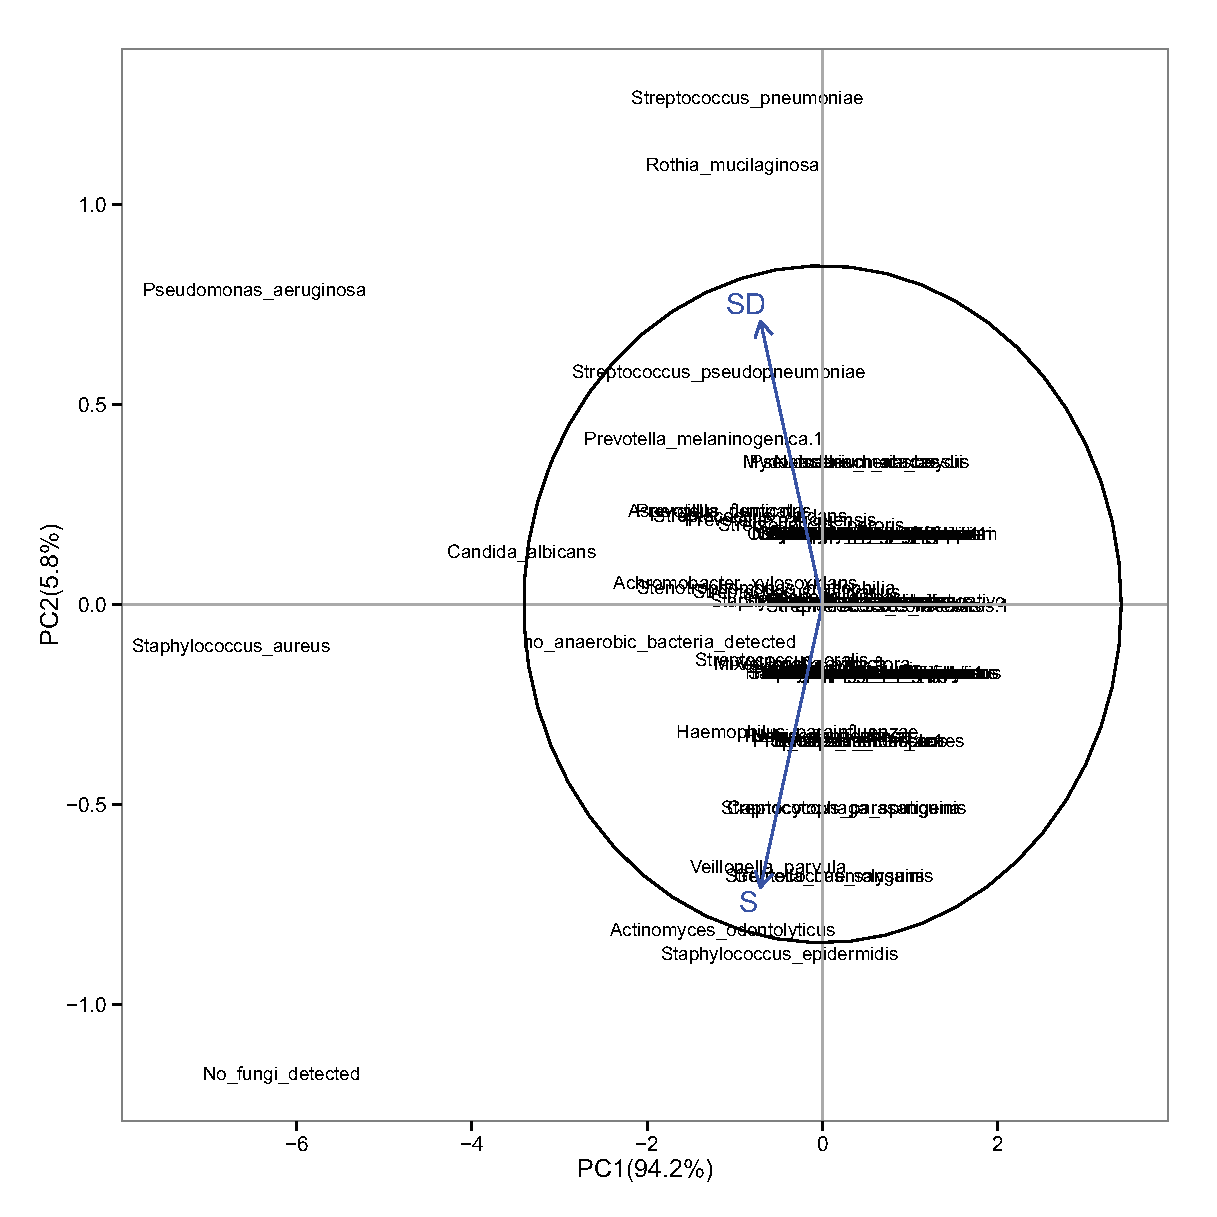
\includegraphics[width=0.8\textwidth]{./figures/Chapter_7/Figure_1_cond_taxa}
  	\caption{\label{fig:fig1condtaxa}Biplot of the principal component analysis of culturable taxa from 78 specimens of stable (S) and substantial decliners (SD) patients with CF. Ellipse with 95\% CI is reported. Numbers on axes indicate the amount of variance explained by each component. Labels outside the 95\% ellipse have been jittered to avoid overlaps.}
\end{figure}%
Principal Component analysis (PCA) of the culturable microflora detected from S and SD samples did not reveal any clear distinction between S and SD groups, neither among the three different clinical conditions examined (I, normal/mild lung disease; II, moderate disease; III, severe disease) (Figure S1). Interestingly, when PCA was performed using the detected taxa as centroids, differences in the microbial community composition between S and SD groups were found. Figure~\ref{fig:fig1condtaxa} shows that \textit{Pseudomonas aeruginosa}, \textit{Rothia mucilaginosa}, \textit{Streptococcus pneumoniae, }and \textit{Candida albicans} for SD group, the absence of fungi and \textit{Staphlyoccoccus aureus} for S group are the most important taxa in contributing to variance differences among S and SD patients in our dataset (in terms of taxa outside the confidence ellipse 95\%, which group  the most similarly occurring taxa).\\
\begin{table}
\centering
\scriptsize
\begin{tabular}{l c c}
\hline
a) SD vs. S patients &  & \\		
Taxon & OR & CI 95\% (lower - upper) \\
\hline\hline
Streptococcus pneumonia & \textbf{9.95} & \textbf{1.47 - 233.90} \\
Rothia mucilaginosa & \textbf{4.87} & \textbf{1.03 - 38.80} \\
Pseudomonas aeruginosa & 1.66 & 0.66 - 4.20 \\
Candida albicans & 1.04 & 0.39 - 2.79 \\
Staphylococcus aureus & 0.86 & 0.34 - 2.18 \\
absence of fungi & 0.77 & 0.30 - 1.96 \\
  &  &  \\
b) FEV\textsubscript{1} (III) vs. FEV\textsubscript{1} (I) + (II) &  & \\
Taxon & OR & CI 95\% (lower - upper) \\
\hline\hline
Candida albicans & 1.57 & 0.53 - 4.55 \\
Pseudomonas aeruginosa & 1.46 & 0.40 - 4.94 \\
No anaerobic bacteria & 1.46 & 0.40 - 4.94 \\
\hline
\end{tabular}
\caption{\label{tab:ortrflp}Odds Ratio from culturable microflora with differential occurrence in SD and S patients and FEV\textsubscript{1} groups. Data report the taxa detected from Principal Component Analysis (Figure~\ref{fig:fig1condtaxa}), the Odds Ratio (OR) of association between presence of the taxa and SD status (a) or FEV\textsubscript{1} (III) with respect to a cohort composed by FEV\textsubscript{1} (I) and FEV\textsubscript{1} (II) patients (b), the 95\% confidence intervals (CI 95\%). Statistically significant ORs are reported in bold. FEV\textsubscript{1}, group I = normal/mild (FEV\textsubscript{1}\% {\textgreater} 70); FEV\textsubscript{1}, group II = moderate (70 ${ \geq}$ FEV\textsubscript{1}\% ${\geq}$ 40); FEV\textsubscript{1}, group III = severe (FEV\textsubscript{1}\% {\textless} 40).}
\end{table}
To statistically evaluate the relationships between the differential presence of these taxa and the patients' status, Odds Ratio (ORs) were computed (Table~\ref{tab:ortrflp}). Statistically significant ORs for SD were found for the presence of \textit{S. pneumoniae} (OR=9.954) and \textit{R. mucilaginosa} (OR=4.867) (Table~\ref{tab:ortrflp} (a)). However, taking account the possible confounders in a logistic regression (Table SM3) for \textit{S. pneumonia }OR was 1.12 (CI 0.14-6.11) and \textit{R. mucilaginosa} OR was 7.37 (CI 1.45-44.41). In the same model \textit{P. aeruginosa} OR was 1.14 (CI 0.34-3.87), while \textit{C. albicans, S. aureus }and absence of fungi had ORs of 2.30, 1.04 and 0.57, respectively.\\%
\begin{figure}[!tb]
	\centering
	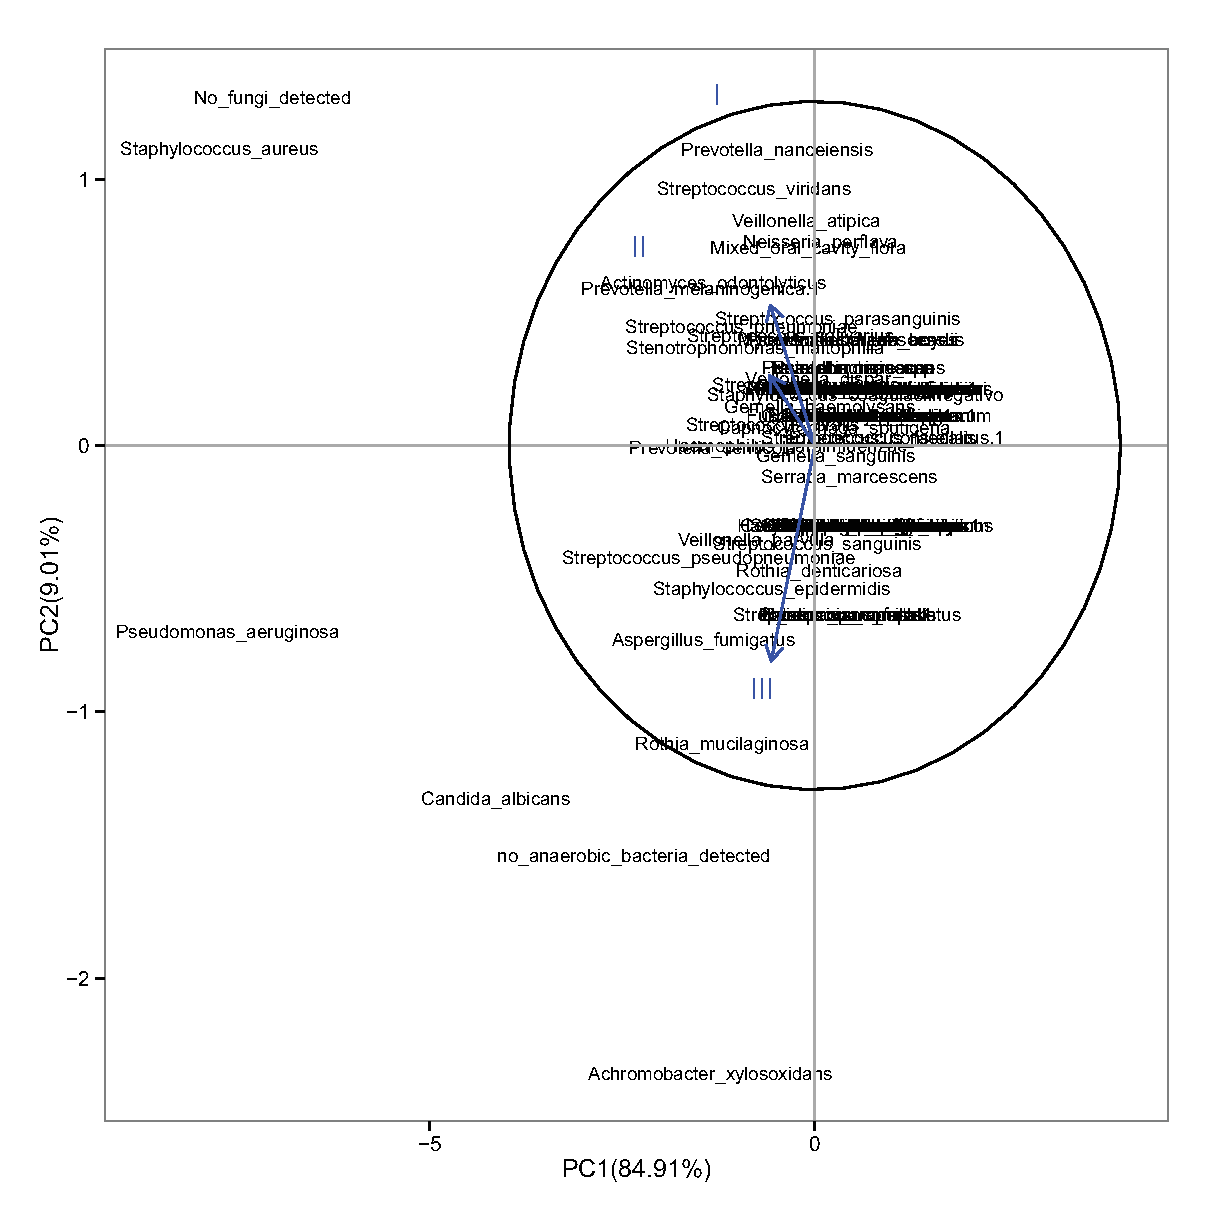
\includegraphics[width=0.8\textwidth]{./figures/Chapter_7/Figure_2_fev1_taxa}
  	\caption{\label{fig:fig2fev1taxa}Biplot of the principal component analysis of culturable taxa from 78 specimens of patients with CF considering their FEV\textsubscript{1} groups. Ellipse with 95\% is reported. Numbers on axes indicate the amount of variance explained by each component. Labels outside the 95\% ellipse have been jittered to avoid overlaps.}
\end{figure}%
When the three different FEV{\textsubscript{1}} groups were considered, PCA showed a differential occurrence of \textit{Achromobacter xylosoxidans},\textit{P. aeruginosa},\textit{C. albicans} as well as the absence of an anaerobic microflora in CF patients with severe lung disease (group III) (Figure~\ref{fig:fig2fev1taxa}). Conversely, for the presence of \textit{A. xylosoxidans} no statistical support could be obtained, since this species was detected only in one patient of group III. Considering ORs for the FEV\textsubscript{1} of group III, in comparison with FEV \textsubscript{1} I and II groups (Table~\ref{tab:ortrflp} (b)), no statistically significant ORs were detected between culturable microflora and FEV\textsubscript{1} decline. By applying a logistic regression including confounders the same result was found (Table SM4), with no detectable limit for the lower confidence interval.\\
\begin{table}
\centering
\scriptsize
\begin{tabular}{l c c c}
\hline
Bacterial communities & \multicolumn{3}{c}{Diversity indices} \\
\hline\hline
a) Culturable microflora & Shannon & Evenness & Richness \\
\hline
SD & 1.64 {\textpm} 0.39 & 0.37 {\textpm} 0.06 & 5.6 {\textpm} 2.3 \\
S & 1.65 {\textpm} 0.40 & 0.36 {\textpm} 0.06 & 5.7 {\textpm} 2.4 \\
  &  &  &  \\
b) T-RFLP community profiles &  &  \\
\hline
SD & 1.89 {\textpm} 0.55 & 0.43 {\textpm} 0.18\textsuperscript{a} & 19.8 {\textpm} 11.0 \\
S & 1.86 {\textpm} 0.56 & 0.52 {\textpm} 0.18\textsuperscript{b} & 16.5 {\textpm} 10.8 \\
  &  &  &  \\
c) T-RFLP profiles / FEV\textsubscript{1} groups &  &  \\
\hline
FEV\textsubscript{1} group I & 1.95 {\textpm} 0.49\textsuperscript{a} & 0.45 {\textpm} 0.17 & 19.7 {\textpm} 9.5 \\
FEV\textsubscript{1} group II & 1.59 {\textpm} 0.48\textsuperscript{b} & 0.47 {\textpm} 0.22 & 15.1 {\textpm} 11.9 \\
FEV\textsubscript{1} group III & 2.09 {\textpm} 0.61\textsuperscript{a} & 0.53 {\textpm} 0.15 & 19.6 {\textpm} 11.6 \\
\hline
\end{tabular}
\caption{Diversity estimates for bacterial communities in sputum samples of CF patients. Data show the mean indices for substantial decliners (SD) and stable (S) patients {\textpm} standard deviation. For T-RFLP data, the indices for the three FEV\textsubscript{1} groups are also reported. Different letters indicate statistically significant (P{\textless}0.05) differences after one-way ANOVA and Tukey \textit{post-hoc} comparison.\label{tab:divtrflp}} 
\end{table}
Concerning the overall values of diversity indices, no statistically significant differences in alpha diversity values were found between the whole groups of SD and S patients (Table~\ref{tab:divtrflp} (a)) as well as between SD and S patients belonging to the severe group (FEV\textsubscript{1} group III), and among the three FEV{\textsubscript{1}} sub- roups in both SD and S patients (data not shown). Furthermore, no significant correlation was found between diversity indices and FEV\textsubscript{1} values (as Pearson's r, p value was \textless 0.9 for all indices).\\

\subsubsection{Total microbiota in S and SD CF patients}
\paragraph{Community composition: species absence/presence} In the 78 sputum samples analyzed by T-RFLP, a total of 1411 bands representing 208 different T-RF lengths were detected. The number of individual bands in each sample ranged from 2 to 43. In particular, ranges were from 3 to 43 for the S patients and 2 to 39 for the SD patients. The mean number of T-RF bands per patient in S sample set (20.2 {\textpm} 11.4) was higher than that of the SD sample (15.5 {\textpm} 10.2), though the difference was not significant (P {\textless} 0.06). Among the 208 T-RF bands detected, 82 (39.4\%) were ``singletons'' defined here as bands that occurred in only one sample. Singletons were detected in 18 (45\%) S and 10 (27.2\%) SD samples.\\
\paragraph{Bacterial community structure} PCA carried out on single patient's T-RFLP profiles did not reveal any clear differences between S and SD patients, nor any differences associated with lung disease status (Figure SM1). When PCA was performed on the markers (T-RFs) as centroids, several (16) T-RFs with a differential contribution toward SD and S (as those outside the confidence ellipse at 95\%) were found (Figure~\ref{fig:fig3condtrf}). Identified T-RFs outside the 95\% confidence ellipse in the biplot were putatively assigned to bacterial taxa by \textit{in silico} digestion with \textit{Cfo}I, using the Phylogenetic Assignment Tool (PAT+) provided by Microbial Community Analysis III (MiCA 3) (\href{http://mica.ibest.uidaho.edu/}{http://mica\-.ibest\-.uidaho\-.edu}). Phylogenetic assignment of the T-RFs was grouped at the phylum level.\\%
\begin{figure}[!tb]
	\centering
	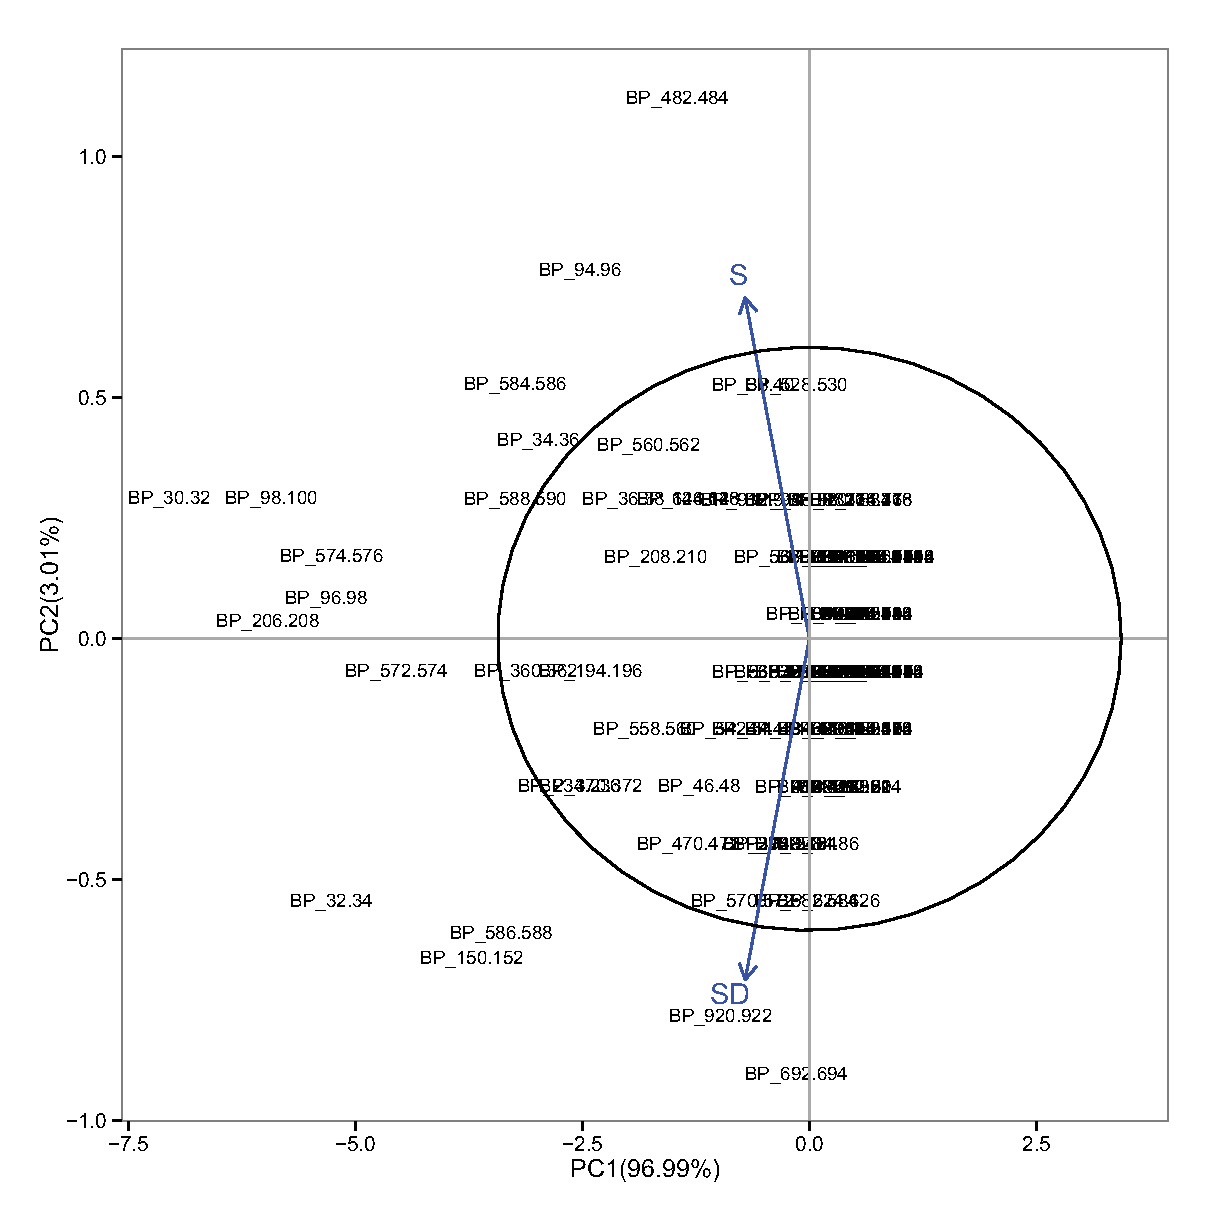
\includegraphics[width=0.8\textwidth]{./figures/Chapter_7/Figure_3_cond_trf}
  	\caption{\label{fig:fig3condtrf}Principal Component Analysis of total occurrences of T-RFs in 78 patients with CF from S and SD patients. Ellipse with 95\% is reported. Comparison of stable with substantial-decliners CF patients. Numbers on axes indicate the amount of variance explained by each component. Labels outside the 95\% ellipse have been jittered to avoid overlaps.}
\end{figure}%
One T-RF (920-922 nt) resulted to have a higher impact on the variance of SD status, while another T-RF (482-484 nt) contributed more to the variance of S status. Moreover, the T-RF at 692-694 nt was only detected in SD patients (in eight out of 38 patients, corresponding to approx. 21\%). A query launched on MiCA 3 web server against the database of 16S rRNA gene sequences allowed to putatively assign 10 out the above mentioned 16 T-RFs to known bacterial taxa. To statistically evaluate the relationships between the differential presence of these taxa and the patients' status, ORs were computed for TFs, too (Table~\ref{tab:ordettrflp}). In particular, T-RFs with OR {\textgreater} 1 (Table~\ref{tab:ordettrflp} (a), i.e., more present in SD than in S patients) enabled to detect \textit{Pseudomonas}, \textit{Shewanella}, and \textit{Burkholderia}. Interestingly, a T-RF putatively assigned at \textit{Shewanella - Colwellia} (920-922 nt) resulted with a high OR for SD patients. The logistic regression model was well in agreement with CMLE ORs estimates (Table SM5). However, several T-RFs were not assigned to any known cultured taxon nor can be assigned to any 16S rRNA gene sequence present in the database (unidentified), including the T-RF at 482-484 nt which is indicated as more frequent in S patients (OR {\textless} 1).\\
\begin{table}
\centering
\tiny
\begin{tabular}{l c c l}
\hline
TRF size (nt) & OR & CI 95\% (lower - upper) & Putative taxonomic attribution \\
\hline\hline
a) SD vs S &  &  &  \\	
\hline
30-32 & 0.94 & 0.26 - 3.39 & Burkholderia \\
32-34 & 2.05 & 0.79 - 5.51 & Burkholderia, Streptomyces \\
34-36 & 0.79 & 0.31 - 1.98 & Anaerofilum, uncultured \\
94-96 & 0.56 & 0.21 - 1.43 & Chloroflexi, Bacteroidetes, uncultured \\
96-98 & 0.28 & 0.06 - 1.06 & Pseudoalteromonas, uncultured \\
98-100 & 0.93 & 0.33 - 2.64 & Cycloclasticus, Mannheimia, uncultured \\
150-152 & 2.04 & 0.83 - 5.15 & uncultured \\
206-208 & 1.18 & 0.44 - 3.17 & Pseudomonas, uncultured \\
482-484 & \textbf{0.29} & \textbf{0.08 - 0.88} & unidentified \\
572-574 & 1.25 & 0.50 - 3.13 & Pseudomonas, Shewanella \\
574-576 & 1.04 & 0.40 - 2.68 & Shewanella \\
584-586 & 0.72 & 0.29 - 1.79 & uncultured \\
586-588 & 2.04 & 0.83 - 5.15 & unidentified \\
588-590 & 0.89 & 0.36 - 2.20 & unidentified \\
692-694 & n.d. & n.d. - n.d. & unidentified \\
920-922 & 3.61 & 1.06 - 14.37 & Shewanella, Colwellia \\
 &  &  & \\
b) FEV\textsubscript{1} (III) vs FEV\textsubscript{1} (I)+(II) &  &  \\
\hline
208-210 & 2.36 & 0.84 - 6.74 & Pseudomonas \\
194-196 & 2.55 & 0.96 - 6.87 & uncultured \\
234-236 & 2.09 & 0.80 - 5.52 & unidentified \\
572-574 & 2.11 & 0.81 - 5.77 & Pseudomonas, Shewanella \\
96-98 & \textbf{3.00} & \textbf{1.00 - 10.18} & Pseudoalteromonas, uncultured \\
574-576 & 2.15 & 0.78 - 6.34 & Shewanella \\
586-588 & 1.50 & 0.59 - 3.86 & unidentified \\
360-362 & 1.47 & 0.57 - 3.77 & uncultured \\
98-100 & 2.10 & 0.68 - 7.23 & Cycloclasticus, Mannheimia, uncultured \\
206-208 & 1.66 & 0.59 - 4.94 & Pseudomonas, uncultured \\
32-34 & 1.01 & 0.38 - 2.73 & Burkholderia, Streptomyces \\
30-32 & 1.22 & 0.33 - 5.06 & Burkholderia \\
34-36 & 0.70 & 0.26 - 1.83 & Anaerofilum, uncultured \\
560-562 & 0.36 & 0.11 - 1.09 & Cellvibrio, Pseudomonas, uncultured \\
470-472 & 0.40 & 0.10 - 1.33 & uncultured \\
558-560 & \textbf{0.28} & \textbf{0.07 - 0.90} & Halomonas \\
144-146 & \textbf{0.07} & \textbf{0.00 - 0.42} & uncultured \\
150-152 & \textbf{0.25} & \textbf{0.09 - 0.66} & uncultured \\
\hline
\end{tabular}
\caption{\label{tab:ordettrflp} Odds ratio from TRFs with differential occurrence in S and SD patients and FEV\textsubscript{1} groups. Data report the TRFs size in nucleotides (nt), the CMLE Odds Ratio (OR) estimates of association between presence of the TRF and SD status (a) or FEV\textsubscript{1} (III), the 95\% confidence intervals (CI 95\%) and the putative taxonomic attributions with MiCA web server. The reported attributions indicate the main hits retrieved for that particular size. Statistically significant ORs are reported in bold.} 
\end{table}
PCA biplot (Figure~\ref{fig:fig4fev1trf}) showed that the vector of FEV\textsubscript{1} group I has a different orientation with respect to those of the other FEV textsubscript{1} groups, suggesting that some T-RFs can indeed be differentially present. We then computed ORs for the 18 T-RFs outside the ellipse 95\%. Results are reported in Table~\ref{tab:ordettrflp} (b). One T-RF (96-98 nt) resulted to contribute more to the variance of FEV\textsubscript{1} group III, while three T-RFs (558-560 nt, 144-146 nt, 150-152 nt) contributed more to the variance of FEV\textsubscript{1} I and II groups. Putative taxonomic identification carried out on such T-RFs highlighted that most of them cannot be assigned (as uncultured or unidentified). The T-RF at 558-560 nt can indeed be assigned to \textit{Halomonas}. However, though CMLE ORs (Table~\ref{tab:ordettrflp} (b)) showed significant ORs the logistic regression model (Table SM6) did not show supported the data.\\%
\begin{figure}[!tb]
	\centering
	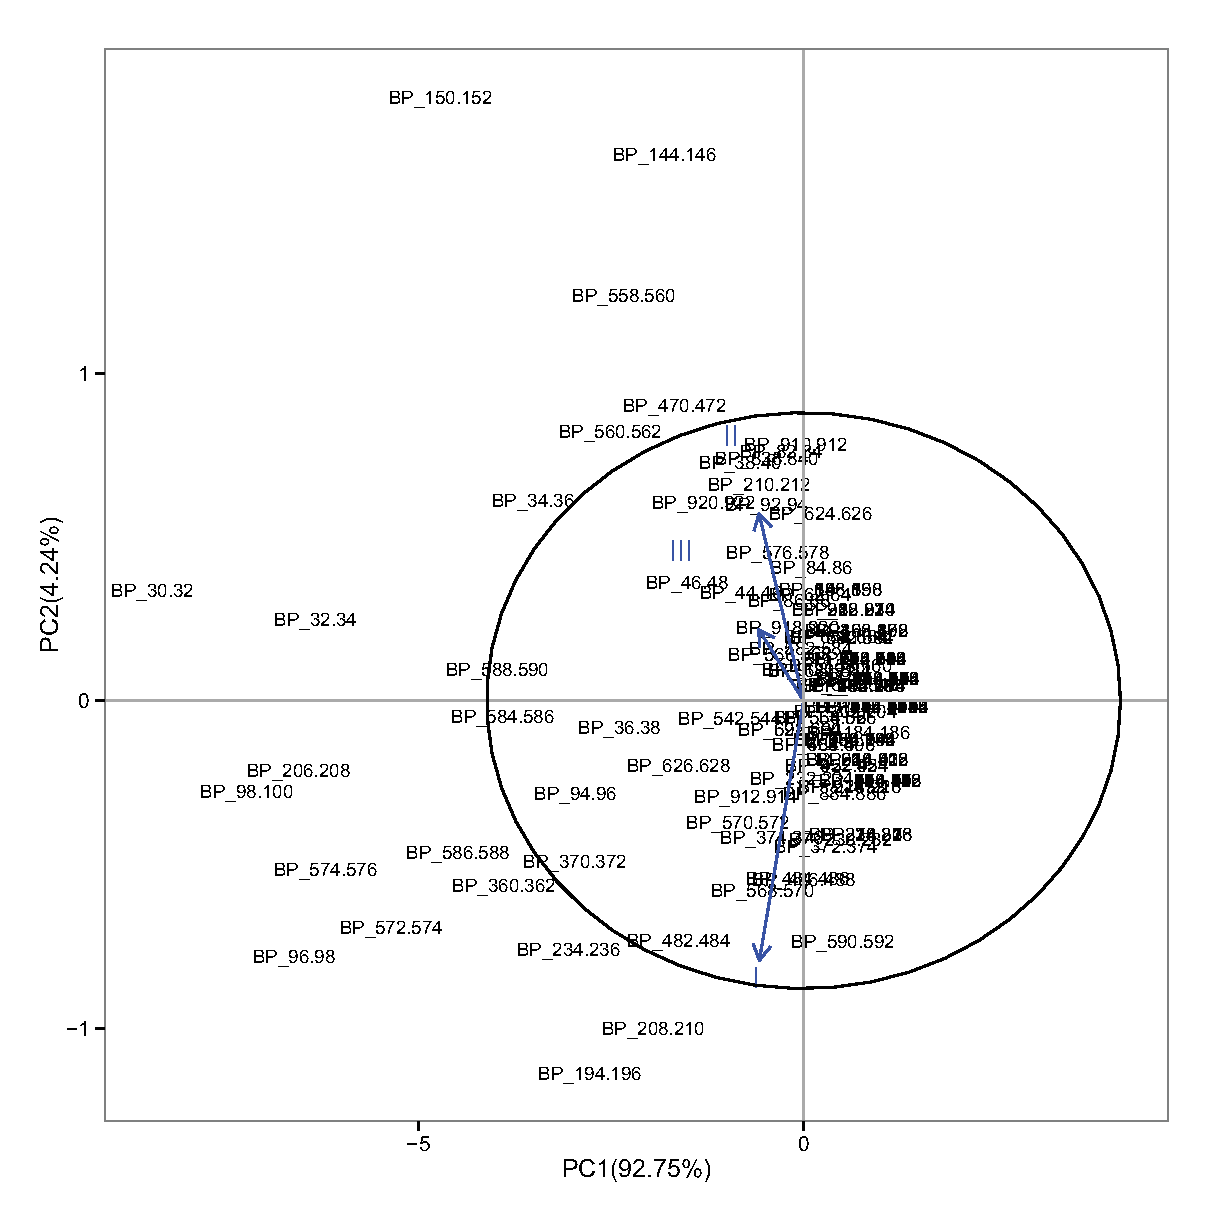
\includegraphics[width=0.8\textwidth]{./figures/Chapter_7/Figure_4_fev1_trf}
  	\caption{\label{fig:fig4fev1trf} Principal Component Analysis of total occurrences of T-RFs in 78 patients with CF from S and SD patients. Ellipse with 95\% is reported. Comparison among FEV\textsubscript{1} groups (I, II, III). Numbers on axes indicate the amount of variance explained by each component. Labels outside the 95\% ellipse have been jittered to avoid overlaps.}
\end{figure}%

\paragraph{Diversity indices} To investigate changes in bacterial communities that may have occurred with severe decline in lung function, diversity indices were computed for all samples by using community ecology parameters (beta diversity estimates). Results revealed that the Evenness, i.e. the equal distribution of T-RFs, resulted higher in S sample set (0.52 {\textpm} 0.18) than in SD sample set (0.43 {\textpm} 0.18) (p {\textless} 0.05). The other diversity indices considered (Richness and Shannon) were not statistically different between the whole dataset of S and SD patients (p {\textgreater} 0.05) (Table~\ref{tab:divtrflp} (b)), and no statistically significant changes were observed between S and SD groups when considering the three FEV\textsubscript{1} sub-groups separately (data not shown). The diversity indices (Evenness, Richness) values did not allow to detect differences among the three FEV textsubscript{1} groups (Table~\ref{tab:divtrflp} (c)), while significant (p{\textless}0.05) differences in Shannon indices of FEV\textsubscript{1} (II) \textit{vs} FEV\textsubscript{1} (I) and of FEV\textsubscript{1} (II)\textit{vs} FEV textsubscript{1} (III) were found. However, no significant differences were found for FEV\textsubscript{1} (I) \textit{vs} FEV\textsubscript{1} (III).\\

\subsection{Discussion}
In the present study, we used both culture-dependent methods for detection of aerobic and anaerobic bacteria and fungi, and a culture-independent method by terminal restriction fragment length polymorphism (T-RFLP), which provide a fingerprint of the most highly abundant members of the community. Data presented here provide new insights into the CF airway microbiota of S and SD patients, population dynamics of the microbiota following lung disease status (normal/mild, moderate and severe lung disease), ecology of the bacterial communities related to lung function decline and establishment of specialized communities of pathogens associated with poor pulmonary function, including putative discriminant microbial species and T-RFs for S and SD groups.\\
The percentage predicted forced expiratory volume in 1 s (FEV\textsubscript{1}\%) is currently the gold standard measure of disease severity in patients with CF. The rate at which FEV\textsubscript{1} declines over a period is an indicator of aggressiveness of a patient's lung disease, regardless of the stage of the patient's lung disease (normal/mild, moderate and severe) \cite{zhao2012decade}. In the present work, we defined as a substantial decline in lung function a decrease of 5\% or more in FEV\textsubscript{1} predicted per year. This percentage drop in FEV\textsubscript{1} suggests a substantial decline similar to that defined by Vandenbranden and colleagues \cite{vandenbranden2012lung} and twice the one reported in published studies \cite{sanders2010failure}. Therefore, the microbiota investigation in CF patients with a more substantial decline in lung function over the previous year can be very useful in order to try to understand where a pathogen is only a marker of disease severity or an independent contributor to the loss of lung function \cite{milla1998risk}.  As ultimately the goal of pulmonary interventions is to retard the disease process and therefore reduce the rate of lung function decline, defining new potential biomarkers for the early detection of severe rate of decline in lung function could be essential for making rational decisions regarding intervention.\\
The presence of \textit{P. aeruginosa} in respiratory tract cultures has been previously reported to be associated with a more rapid decline in lung function, especially when mucoid phenotype is present \cite{emerson2002pseudomonas}. However, Vandenbranden and colleagues \cite{vandenbranden2012lung} found that the presence or absence of \textit{P. aeruginosa} or mucoid \textit{P. aeruginosa} was not predictive of lung function decline. Our findings from culture-based analysis showed that \textit{P. aeruginosa} cannot be strongly proposed as indicative of severe decline in lung function (OR = 1.14, CI 0.34-3.87). It is noteworthy that maintenance treatment for chronic \textit{P. aeruginosa} with inhaled antibiotics and/or azithromicin in accordance with the Guidelines \cite{farrell2008guidelines}. resulted in slowing down the rate of decline in FEV\textsubscript{1}. Our culture-based results suggest an important role of \textit{S. pneumoniae} and \textit{R.mucilaginosa} as marker species for SD status. Although \textit{S.pneumoniae} is a common respiratory tract pathogen, it is unusual in CF \cite{foweraker2009recent}. This bacterial species is able to persist in the CF lung and has been recently regarded as pathogenic within the CF community \cite{maeda2011population}. However, to the best of our knowledge, it is still unclear whether \textit{S.pneumoniae} has a role in acute exacerbation and severe lung decline or can act synergically with other CF pathogens. As regards \textit{R. mucilaginosa}, it was previously reported as an aerobic species isolated from CF sputum \cite{tunney2008detection} and it was defined by several Authors \cite{bittar2008molecular} as a ``new'' emerging CF pathogen. Recently, Lim and colleagues \cite{lim2013mechanistic} confirmed that \textit{R. mucilaginosa} is present and metabolically active in the lungs of CF patients and that it evolves and adapts to each patient's lung environment over the course of a persistent infection. Our results also reinforce the previous findings of Chotirmall and colleagues \cite{chotirmall2010sputum} who reported that colonization with \textit{C. albicans} presages FEV\textsubscript{1} decline in CF. Although the same Authors suggested the implication of \textit{C. albicans} in the decline of CF lung function, the clinical relevance of yeasts is still a matter of debate, and has yet to be confirmed. Our findings add support to $i)$ the pathogenicity of species derived from the oral cavity and usually considered as clinically insignificant, and $ii)$ the complex interaction between typical pathogens and microbiota, such as the association between \textit{P. aeruginosa} and anaerobes/fungi.\\
It is well known that CF airways harbor numerous organisms that evade detection by culture-based methods. To carefully examine the microbiota from patients with stable versus worsening disease status, we chose to utilize T-RFLP analysis to generate community profiles. T-RFLP is a popular molecular profiling technique with the capacity to resolve community members based on the position of restriction sites in the 16S rRNA gene \cite{liu1997characterization}. T-RFLP profiles have been extensively used for community differentiation, identification of specific organisms in microbial populations  and comparison of the relative phylotype richness and community structure in a diverse range of environments \cite{osborn2000evaluation, marsh2005culture, tiquia2010using, joo2010monitoring, nakano2010prediction}. When previously applied to the analysis of spontaneously expectorated sputum from CF patients, T-RFLP has indicated the presence of a diverse array of bacterial species \cite{stressmann2011analysis, rogers2010determining, rogers2003bacterial, sibley2008polymicrobial}. In this study, we used T-RFLP analysis as a tool to investigate two key topics. First, do the bacterial communities (microbiota) detected in S samples differ from those in SD samples? Additionally, are there differences in the microbiota among CF patients with different status of lung disease? Results obtained in the present study by T-RFLP analysis revealed a greater bacterial diversity within sputum samples than that detected by culture approaches. We did not find T-RFLP profiles exclusive of the patients from S or SD groups. T-RFLP analysis revealed sixteen T-RFs as the most differentiating between S and SD groups after PCA. However, in our dataset, significant ORs were only recorded for two of them (and only one was possible to identifiy as putative \textit{Shewanella})Interestingly, the other T-RFs which differentiate (tough not significantly on the basis of ORs) S from SD were putatively identified as belonging to known CF pathogens, as \textit{Pseudomonas} and \textit{Burkholderia}, but most of them resulted in no species assignation (only {\textasciitilde}18\% of T-RF band lengths match a band length generated from published sequence data).Therefore, these unknown T-RFs could be either novel species or related species/strains of the core community of CF airways, but with enough heterogeneity in the 16S rRNA gene that may generate slightly different fragment sizes \cite{camarinha2012validating}. \textit{S.pneumonia} and \textit{R. mucilaginosa} were detected by culturing but not by T-RFLP analysis. It is well known that molecular methods based on 16S sequence data have a limited ability to resolve taxonomic identification at the species level \cite{filkins2012prevalence} and may introduce biases during the primer-binding step of PCR \cite{cai2013biased}. In spite of these limits, and taking also into consideration that T-RFLP only allows a putative (though fast) taxonomic assignment, this culture-independent method adds valuable information to the data obtained from culture analysis. To gain a more comprehensive characterization of CF lung microbial communities, more sophisticated and expensive techniques, such as bacterial metabarcoding by 16S rDNA and metagenomic sequencing \cite{maughan2012analysis, lim2014clinical} will be applied. \\
To investigate changes in bacterial communities that may have occurred with substantial decline in lung function, the diversity indices on T-RFLP data were calculated for all samples. Diversity provides a measure of community complexity based on the number (Richness) and relative abundances (Evenness) of the species present. The reduced Evenness observed in SD respect to S group of patients revealed an impaired ecology of the bacterial community in SD patients, which in turn can be associated with lung function decline experienced by those patients. When we assessed community structures to describe the degree of change occurring in the airway microbiota following the decline in lung function, we did not find a decrease in Shannon diversity index with advanced disease in the SD group. As suggested by Zhao and colleagues \cite{zhao2012decade}, other factors, such as antibiotic use, rather than lung function or patient age have been found to be the primary drivers of the decreasing bacterial diversity in CF patients with progressive lung disease. In our study, patients with a more rapid decline in lung function did not have a higher antibiotic exposure over the previous year with respect to S patients; additionally, both S and SD patients did not receive antibiotics in the 30 days preceding the specimen collection. Collectively, our results suggest that the antibiotic use is not likely to have contributed to the failure in detecting a decrease in community diversity with advanced disease in the SD group. Moreover, we cannot \textit{a priori} exclude that the use of relative peak intensities as a proxy for taxa frequency, though largely used (for instances see  \cite{camarinha2012validating, blackwood2007interpreting, ding2013community}), may be someway biased and can produce altered data. Our analyses suggest that overall bacterial diversity remains relatively stable despite the decreasing in relative abundances of the species in SD patients. Indeed, as previously stated by Zhao and colleagues \cite{zhao2012decade}, community diversity alone is not a sufficient indicator of the disease status. However, considering only the three subgroups of FEV\textsubscript{1} (normal/mild \textit{vs} moderate, \textit{vs} severe), independently from the rate at which FEV textsubscript{1}\% declines, statistically significant differences among the three sub-groups were also found, suggesting that the patients with intermediate FEV\textsubscript{1} values are experiencing changes in the airway assembly of taxa. A more detailed taxonomic and functional analysis of the microbial community of lung microbiota of CF patients could help elucidating the microbial factors that can contribute to such changes.\\ 
In conclusion, by combining culture-dependent and culture-independent methods with ecological tools and clinically relevant information, a more comprehensive view of microbial community composition in SD patients with CF was determined. Overall, our results suggest that the presence of \textit{P. aeruginosa} ``per se'', as well as the single T-RFLP profiles, are not able to define the S or SD group. New biomarkers are required in CF to predict the decline clinical phenotype and monitor the response of CF patients to existing and new therapeutic strategies. Microbial factors represent a potential to provide biomarkers for the early detection of the substantial lung function decline in CF. We have identified some discriminatory species as well as some discriminatory T-RFs, that represent good candidates as predictors of substantial decline in lung function, enabling to stratify individuals with CF at high or low risk of future severe lung function decline. However, only longitudinal studies can help determine patterns of association between the CF airway microbiome and lung disease. A more in-depth investigation of microbial airway bacterial communities in longitudinal studies and by high-throughput sequencing and bioinformatics tools will provide powerful means to better understand the contribution of the airway microbiome to severe decline in FEV\textsubscript{1} and its potential for the development of new biomarkers as predictors of severe pulmonary disease in CF patients.\\

\subsection{Acknowledgements} We thank John LiPuma, Gianni Mastella and late Gerd D\"oring for their helpful suggestions. We dedicate the present article to the memory of Gerd D\"oring (University of T\"ubingen, T\"ubingen, Germany), who was a world authority on infection and inflammation in the CF lung. With Gerd's death, we lost an excellent scientist, a loyal and generous friend, a marvelous speaker, and a charming person of great sensitivity and nobility. We also acknowledge the Italian Cystic Fibrosis Research Foundation (FCC) for its support and administrative tasks, and Graziana Manno, Anna Marchese, Silvia Campana, Gabriella Ricciotti, Cristina Cantale for their valuable assistance. \\

%%%%%%%%%%%%%%%%%%%%%%%%%%%%%%%%%%%%%%%%%%%%%%%%%%%%%%%%%%%%%%%%%%%%%%%%%%%%%%%%%%%%%%%%%%%%%%%%%%%%%%%%%%%%%%%%%%%%%%%%%%%%%%%%%%%%%%%%
%%%%%%%%%%%%%%%%%%%%%%%%%%%%%%%%%%%%%%%%%%%%%%%%%%%%%%%%%%%%%%%%%%%%%%%%%%%%%%%%%%%%%%%%%%%%%%%%%%%%%%%%%%%%%%%%%%%%%%%%%%%%%%%%%%%%%%%%

\section[Taxonomic signatures of CF airway microbiota distinguish between stable and severe declining patients]{Taxonomic signatures of CF airway microbiota distinguish between stable and severe declining patients%
\sectionmark{Taxonomic signatures of CF airway microbiota}}
\sectionmark{Taxonomic signatures of CF airway microbiota}

Cystic fibrosis (CF) is an autosomal recessive genetic disorder characterized by a progressive decline in lung function. Patients with CF may show a rapid and severe decline of their pulmonary efficiency, measured as FEV\textsubscript{1} percentage, despite antibiotic treatment. Usually, these treatments are selected relying on the susceptibility of individual and culturable microbial strains to specific antibiotics in vitro. Nevertheless, this approach may not correctly predict medical outcomes because of both technical and biological factors. In these years, several culture-independent studies have shown that the CF airway infection is significantly more complex and dynamic than previously detected. Thus, understanding the ecological and evolutionary dynamics able to modify the lung microbiota of CF patients is critically important for either developing new and more effective therapies or improving existing ones. In this study, we analyzed the sputum from 52 patients with different disease conditions through 16S rRNA metabarcoding analysis in order to bring an in-depth overview of the lung microbiota at different stages of CF disease. The enrolled patients were divided into 2 main groups based on their rate decline in FEV\textsubscript{1} value per year. Patients with a rate decline greater than -1.5\% were assigned to the ``stable'' group (S), whereas patients with a rate decline between -1.5\% and -5.0\% were assigned to the ``severe decliners'' group (SD). Moreover, patients were further categorized into three FEV\textsubscript{1} groups: group I (FEV\textsubscript{1} {\textgreater} 70\%); group II (FEV\textsubscript{1} ranging from 40\% to 69\%) and group III (FEV\textsubscript{1} {\textless} 40\%). Surprisingly, the metabarcoding analysis has shown that bacterial biodiversity of stable patients dropped down passing from group I to group II of FEV\textsubscript{1} index; whereas bacteria community connection has a similar behavior passing from ``stable'' to ``severe decliners conditions''. Here, we theorize that something (still unknown) is occurring in the ecology of lung microbiota passing from FEV\textsubscript{1} I to FEV\textsubscript{1} II, which may misbalance bacterial community ecology, opening the way to more severe conditions.\\

\subsection{Introduction}
The main goal of pulmonary interventions is to retard the disease process reducing the rate of lung function decline even defining new potential biomarkers for the early detection of severe rate of decline in lung function, essential for taking rational decisions regarding intervention.\\
In recent years the microbial ecology of the airways in cystic fibrosis (CF) has been shown to be significantly more complex than originally considered \cite{lipuma2010changing, rogers2014respiratory}. Recent works using culture-independent identification methods have revealed that CF patients harbor a vast array of bacteria, previously not identified and not suspected to be involved in the infection and inflammation typical of CF patients \cite{zhao2012decade}. During the last few years, the development of next-generation sequencing technologies and bioinformatics tools has enabled the large-scale investigation of microbial communities and has facilitated our understanding of a ``black box'' of microbial communities present in CF airways \cite{delmont2011metagenomic}. These findings have altered drastically our understanding of CF lung disease \cite{rogers2014respiratory}, but their translation into improvements in clinical outcome remains a substantial obstacle to improving the quality of care. It has been proposed that the lung microbial communities might be considered as a unique distinct pathogenic entity, whose impact on the host may be greater than the combined impacts of its individual component species alone \cite{rogers2010comparing}. Indeed, an ecological perspective on multispecies colonization of the CF airways will permit to understand the role of polymicrobial dynamics in CF lung disease and provide the clinicians with new biomarkers of CF progression, as well as with new bacterial targets for antibiotic treatment \cite{sibley2008polymicrobial}.\\
Until now, many efforts have been made to identify microbes associated with airway diseases, antibiotic treatment, patient age increasing, and periodic pulmonary exacerbation \cite{zhao2012decade, cox2010airway, carmody2013changes, zhao2014modeling, zemanick2013inflammation}. However, it is still not clear how changes in the airway microbiota composition are predictive of severe lung disease progression. Bacterial infections in the CF airways are currently monitored through routine microbiology and CF patients receive cures based on culturable microbial pathogens colonizing their airways \cite{flume2009cystic}. It has been found that the administration of antimicrobial therapy, based on the in vitro susceptibilities of classic CF pathogens, does not necessarily correlate with the clinical outcome \cite{sibley2009relevance}.\\
Here we used 16S rRNA metabarcoding analysis of lung microbiota to describe the ecological issues (biological diversity, taxa composition, interaction among taxa) related to a specific pulmonary physiopathological status. We analyzed the microbiota of a large cohort of patients (a total of 52 patients) differing for status (S and SD) and FEV\textsubscript{1} index values in order to explore how bacterial communities change during the course of CF disease.\\

\subsection{Materials and Methods}

\subsubsection{Ethics Statement}
Sputum samples from patients with CF were collected at Bambino Ges\`u Children's Hospital (Rome, Italy), Cystic Fibrosis Center, Meyer Children's Hospital (Florence, Italy) and Giannina Gaslini Children's Hospital (Genoa University, Genoa, Italy), in accordance with the ethical guidelines. The study was approved by the local Ethics Committee of each participating Center [Prot. 85 of February 27, 2014 (Meyer Children's University Hospital); Prot. n. 681 CM of November 2, 2012 (Bambino Ges\`u Children's Hospital); Prot. n FCC 2012 Partner 4-IGG of September 18, 2012 (Giannina Gaslini Institute)]. Informed written consent was obtained from all subjects aged 18 years and over and from parents of all subjects under 18 years of age prior to enrollment in the study. The study protocol was in accordance with the Guidelines of the European Convention of Human Rights and Biomedicine for Research in Children and to those of the Ethics Committees of Bambino Ges\`u, Meyer and Giannina Gaslini Hospitals. All measures were taken to ensure patient data protection and confidentiality.\\

\subsubsection{Patients}
52 patients attending three Italian CF Centers (Bambino Ges\`u Children's Hospital, Rome; CF Center, Meyer Children's Hospital, Florence; and Giannina Gaslini Children's Hospital, Genoa) were enrolled in the study between September 2012 and April 2013. Patients, who had been diagnosed with CF according to the published Guidelines \cite{farrell2008guidelines}, were treated by following such Guidelines and consensus for lung monitoring with at least four microbiological controls per year \cite{flume2009cystic}. Patients were eligible if they could be classified as clinically stable, without any pulmonary exacerbation and antibiotic e.v. or oral therapy in the previous 4 weeks \cite{fuchs1994effect, ramsey1999intermittent}.\\
The annualized rate of FEV\textsubscript{1} decline was used to stratify patients as previously reported. CF patients were categorized as ``stable'' (S), i.e. with a rate decline in FEV\textsubscript{1} value no greater than -1.5\% per year, and with a ``substantial decline'' (SD) in FEV\textsubscript{1}, i.e. a rate of FEV\textsubscript{1} decline greater than - 5\% predicted per year. Both S and SD patients were further categorized in three FEV\textsubscript{1} groups: group I, CF patients with normal lung function or mild lung disease (FEV\textsubscript{1} {\textgreater} 70\%); group II, CF patients with a moderate lung disease (FEV\textsubscript{1} ranging from 40\% to 69\%); group III, CF patients with a severe lung disease (FEV\textsubscript{1} {\textless} 0\%). FEV\textsubscript{1} values were measured according to the American Thoracic Society-European Respiratory Society standards \cite{miller2005standardisation}. The overall description of the patient dataset is reported in Table SM1. For additional details on patients number and the number of sequences generated for each group of patients see Table~\ref{tab:ffc116s}.\\
\begin{table}
\centering
\scriptsize
\begin{tabular}{c c c c}
\hline
FEV1 & Condition & \# Patients & \# Sequences \\
\hline\hline
I & S & 13 & 35746 \\
II & S & 10 & 29462 \\
III & S & 6 & 19499 \\
I & SD & 10 & 31332 \\
II & SD & 7 & 20121 \\
III & SD & 6 & 21947 \\
Total &  & 52 & 158107\\
\hline
\end{tabular}
\caption{\label{tab:ffc116s}Number of enrolled patients in each group. The table reports also the number of amplicon sequences assigned to each group.} 
\end{table}

\subsubsection{Sample processing and DNA extraction} 
The analysis of the bacterial community composition was performed on spontaneously expectorated sputum (SES) samples since sputum specimen represents by far the most widely used sample in productive patients \cite{rogers2010comparing}. Samples processing was performed as previously described. About 400 {\textmu}l aliquots of frozen sputum were subjected to genomic DNA extraction using the commercially-available Kit QIAamp DNA Mini Kit. Sample aliquots were spun at 10,000{\texttimes}g to pellet cellular material. After removal of the supernatant, cell pellets were resuspended in 180 {\textmu}l of enzyme solution (20 mg/ml lysozyme in 20 mM Tris{\textperiodcentered}Cl, pH 8.0, 2 mM EDTA, 1.2\  Triton), incubated for 30 min at 37{\textdegree}C and then processed according to the manufacturer's protocol. Quantity and purity of extracted DNA were checked by NanoDrop (NanoDrop Technologies, USA) and PicoGreen fluorescent assay (Life Technologies) and gel electrophoresis.\\

\subsubsection{Amplification and barcoding of bacterial 16S rRNA gene amplicons}
Fifty-four samples (from 52 patients) were obtained and subjected to 16S rRNA gene amplification. The V3, V4, and 5 hypervariable regions of the 16S rRNA gene were amplified using primer 357F (5'-CTA\-CGG\-GAG\-GCA\-GCA\-G-3') modified with the addition of the 454 FLX-titanium adaptor ``B'' sequence (5'-CTA\-TCC\-CCT\-GTG\-TGC\-CTT\-GGC\-AGT\-CTC\-AG-3') and primer 926R (5'-CCG\-TCA\-ATT\-CMT\-TTR\-AGT-3') modified with the addition of 18 unique seven-nucleotide barcode sequences (MID 1 - MID 18, Roche MID adapters) and the 454 FLX titanium adaptor ``A'' sequence (5'-CCA\-TCT\-CAT\-CCC\-TGC\-GTC\-CAT\-CTC\-ATC\-CCT\-GCG\-TGT\-CTC\-CGA\-CTC\-AG-3').\\
Primer design and barcode sequences were as previously reported by Human Microbiome Project (HMP) Consortium \href{http://www.hmpdacc.org/tools\_protocols/tools\_protocols.php}{http://\-www\-.hmp\-dacc\-.org/\-tools\_proto\-cols/\-tools\_pro\-to\-cols\-.php}.\\
PCR amplification was performed on 30 {\textmu}g of DNA template in a total volume of 25 {\textmu}L containing 1{\texttimes} AccuPrime Buffer II (Life Technologies), 10 {\textmu}M of 357F fusion-primer, 10 {\textmu}M of 926F fusion-primer and 0.03 U/{\textmu}L AccuPrime High-Fidelity \textit{Taq} DNA polymerase (Life Technologies). PCR reactions were heated at 95 {\textdegree}C for 2 min followed by 30 cycles of 95 {\textdegree}C for 20 s, 55 {\textdegree}C for 30 s, and 72 {\textdegree}C for 5 min. All reactions were prepared in a sterile PCR hood. Three independent 25 {\textmu}L PCR reactions were generated for each patient DNA-template. Negative control reaction (no DNA template) were also performed. 2.5 {\textmu}L of each replicate reactions were examined by electrophoresis on an 1,5 \% agarose gel. PCR amplicons were cleaned using the Agencourt AMPure XP Beads according to the manufacturer's specifications (Beckman Coulter). To ensure removal of primers and any nonspecific amplicons, purified amplicon libraries were analyzed using the Agilent Bioanalyzer 2100 employing the Agilent DNA 1000 Kit. The concentration of the purified amplicons was determined using the Quant-iT PicoGreen dsDNA fluorescent assay Kit (Life Technologies).\\
For each patient sample, the three independent purified and quantified PCR reactions were pooled in an equimolar ratio of 109 molecules {\textmu}l-1. Amplicon pools were quantified using KAPA Library Quantification Kits (KAPA Biosystems) to determine exactly the number of amplifiable molecules in the amplicon libraries. For 16S Amplicon qPCR reactions two dilutions (1:500 and 1:1000) of each purified library were used. qPCR amplification was performed on 4 {\textmu}L of Amplicon library template in a total volume of 10 {\textmu}L containing 6 {\textmu}L of KAPA SYBR{\textregistered} FAST qPCR Master Mix. Reactions were heated at 95 {\textdegree}C for 5 min followed by 35 cycles of 95 {\textdegree}C for 30 s, and 60 {\textdegree}C for 90 s. In addition, dissociation (melt curve) analysis was performed to provide indication of possible primer- and/or adaptor-dimer contamination of libraries.\\ The concentration of each Amplicon library in molecule/{\textmu}L was achieved by inference from a standard curve generated using the six DNA Standard included in KAPA Library Quantification Kits.\\

\subsubsection{Amplicon Library Amplification and Pyrosequencing} 
To clonally amplify the amplicon libraries, the optimal amount of DNA to use in emPCR amplification was determined using emulsion titration procedure according to the supplier's instructions described in ``emPCR Amplification Manual'' (454 Life Sciences Roche Corporation). Before emulsion titration, MID-containing libraries (MID1 to MID18) were normalized to the same molecule concentration, pooled in equal volumes, and diluted to the emulsion PCR working concentration according to the supplier's instructions described in ``emPCR Amplification Manual'' (454 Life Sciences Roche Corporation). Overall, 3 equimolar amplicon library pools were prepared and purified with AMPure XP beads. Emulsion PCR, emulsion breaking and amplicon pyrosequencing were performed applying the 454 GS FLX+ chemistry following supplier protocols (454 Life Sciences Roche Corporation). Sequencing of amplicons was conducted on a 454 GS FLX+ System (454 Life Sciences Roche Corporation); each of the 3 amplified amplicon libraries was loaded on a PicoTiterPlate (PTP) device, using 3 regions of a medium regions ``4-lane'' gasket. The latest GS FLX+ software 2.9 version was used to sequencing and the pipeline 3 for long amplicon was used to data processing (454 Life Sciences Roche Corporation).\\

\subsubsection{Sequence processing and data generation}
Sequences generated via pyrosequencing were separated from the run according to their barcode sequence using custom bash and Java scripts available upon request. Sequences possessing primer mismatches higher than 2 bp were discarded in order to assign to each sample (patient) only sequences with an almost perfect match with the barcode. A quality check step was performed using StremingTrim 1.0 \cite{bacci2014streamingtrim} a very conservative algorithm able to retain as much information as possible. Sequences were then trimmed to a fixed length (568 - 572 bp) while low quality sequences were removed from the analysis. Processed sequences were subjected to the UPARSE pipeline \cite{edgar2013uparse} in order to remove chimeric sequences (both in de novo and in reference mode) and to cluster them into Operational Taxonomic Units (OTUs). An identity threshold of 97\% has been used in this step to be able to analyze the lung bacterial community at a high resolution level. Indeed, a 97\% identity threshold of the 16S rRNA gene corresponds approximately to the taxonomic level of species \cite{konstantinidis2007prokaryotic}. Representative sequences obtained from the UPARSE clustering were taxonomically classified using the SINA standalone classifier combined with the most recent SILVA database available (SSU 115). For additional details on the number of OTUs assigned to each patient see Table SM1.\\
OTU counts were normalized to relative abundance by dividing the number of assigned sequences by the sample size (number of sequences assigned to each patient) before comparing bacterial community from different samples. Prevalence values were calculated as the fraction of samples containing a given OTU whereas abundance values were computed as the fraction of reads assigned to a particular OTU. For taxonomic data generation, all OTUs assigned to the same taxa were summed together and normalized as described above.\\

\subsubsection{Statistical analyses}
OTUs counts were rarefied according to the lowest abundant sample in order to be able to compute and compare biodiversity indices of all samples. Shannon, Richness and Evenness indices were calculated on rarefied sequence counts repeating the rarefaction step 1000 times. An Analysis of Variance (ANOVA) has been performed to inspect differences in bacterial community diversity related to clinical conditions. In particular, Forced Expiratory Volume (FEV\textsubscript{1}) and patient conditions (Stable or Severe Decline) have been considered in the analysis. Moreover, to confirm results obtained with the ANOVA analysis, a Multivariate Analysis of Variance (MANOVA) was performed on the whole bacterial dataset. Finally, a Canonical Correlation Analysis (CCA) has been carried on to be able to visualize results and inspect the effect of the two factors reported above. Before performing the CCA analysis, the abundance (represented by number of sequences) of the OTUs was log transformed for normalization. All statistical analyses were performed with the R software \cite{team2012r} and the vegan package \cite{oksanen2007vegan}.\\

\subsubsection{Network construction}
In order to generate network representations of the lung bacterial community, all possible Spearman's rank correlation have been calculated between OTUs. A co-occurrence event has been considered valid only if the Spearman's correlation coefficient was higher than 0.6 and statistically significant with a p-value lower than 0.05. Two distinct networks were generated (one including Stable patients and the other considering Severe Decline patients) were each node correspond to a different OTU and each edge represent the presence of a statistically significant Spearman's correlation {\textgreater} 0.6 between OTUs. The diameter of the nodes was directly proportional to the OTU relative abundance in the dataset. The same approach has been used to construct other three networks, one for each FEV\textsubscript{1} level. All statistical analyses were carried out in the R environment using the igraph package for network generation.\\

\subsection{Results}
\subsubsection{Taxonomic description}
In the sputum microbiota analyzed a total of 44 OTU were detected, with values ranging from 1 to 4334 (Table SM2). The relative abundance values of each identified genus are reported in Figure~\ref{fig:fig116s}. A large heterogeneity was found for all patients, and such heterogeneity in relative taxa abundance was also present at higher taxonomic levels (Figure SM 1).\\%
\begin{figure}[!tb]
	\centering
	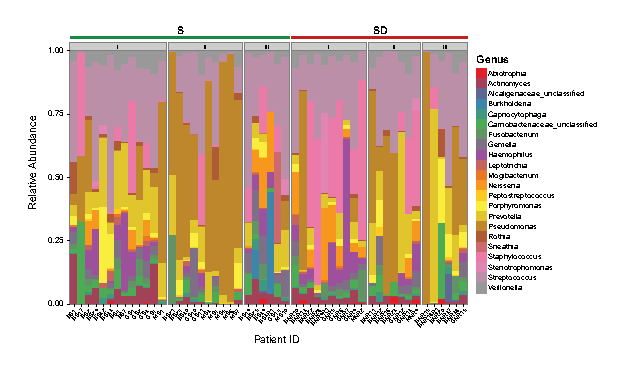
\includegraphics[width=1\textwidth]{./figures/Chapter_7/Figure_1_16s}
  	\caption{\label{fig:fig116s}Segmented bar plot reporting relative abundances of OTU counts collapsed at Genus taxonomy level. OTU counts were transformed to relative abundance by dividing the number of assigned sequences by the sample size. Each bar of this plot reports the relative abundance of all genera detected in a sample (patient). The bar colors represent the different genera detected.}
\end{figure}%
When the bacterial distribution at genus level was analyzed in terms of prevalence and abundance between groups (Figure~\ref{fig:fig216s}), similar patterns in all groups (S vs. SD at different FEV\textsubscript{1} groupings) were found for genera belonging to \textit{Actinobacteria}, \textit{Bacteroidetes}, \textit{Firmicutes} and \textit{Fusobacteria}. On the contrary, genera belonging to \textit{Proteobacteria }showed a more variable pattern. In particular, \textit{Pseudomonas} assignments within the SD group showed a pattern of increasing prevalence and abundance following FEV\textsubscript{1} groups. In the S group, \textit{Pseudomonas} assignments showed high levels of prevalence and abundance in the group II of FEV\textsubscript{1} only.\\%
\begin{figure}[!tb]
	\centering
	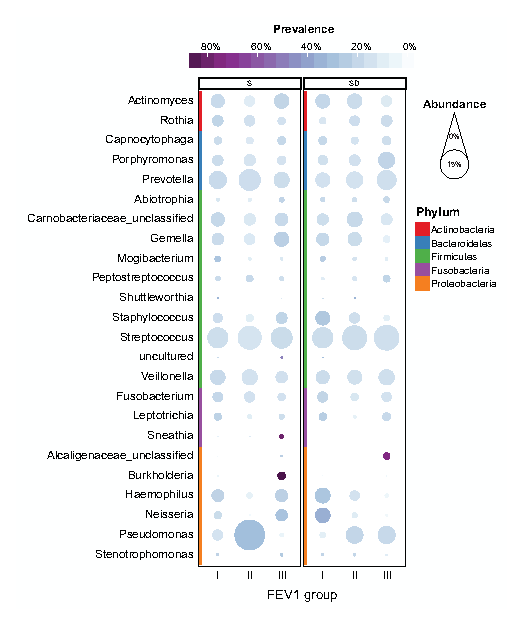
\includegraphics[width=0.7\textwidth]{./figures/Chapter_7/Figure_2_16s}
  	\caption{\label{fig:fig216s} Abundance and prevalence of detected taxa in CF patients. Prevalence (intensity of color) and abundance (size) of clades in the lung microbiome. Taxa belonging to the same Phylum were grouped together reporting a different color for each Phylum detected.}
\end{figure}%

\subsubsection{Statistical evaluation of lung microbiota differences}
Rarefaction curves (Figure~\ref{fig:fig316s}) showed that all samples had the required amount of sequences to assess OTU richness (all curves reached an asymptote). After normalization of bacterial counts to relative abundance values, biodiversity indices have been calculated (Table SM3) and a two-factor Analysis of Variance (two-factor ANOVA) was carried out in order to evaluate if biodiversity values differed in relation to both patient status (S vs. SD) and pulmonary functionality (FEV\textsubscript{1} groups) (Table~\ref{tab:ffc216s}). %
\begin{figure}[!tb]
	\centering
	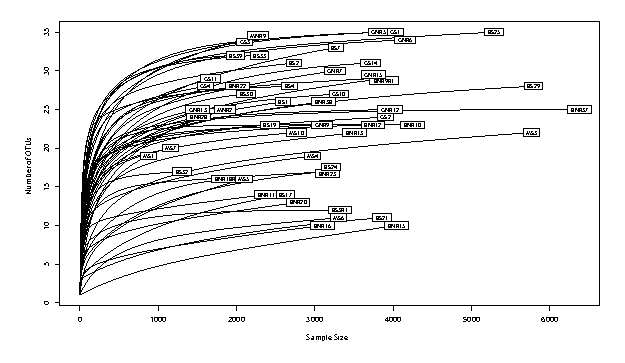
\includegraphics[width=0.8\textwidth]{./figures/Chapter_7/Figure_3_16s}
  	\caption{\label{fig:fig316s} Rarefaction curves calculated for sputum samples of all patients. A curve has been drawn for each sample with the sample ID reported at the end. As showed in this figure, all curves reached an asymptote whereas samples have not achieved the same number of sequences.}
\end{figure}%
Regarding both Evenness and Shannon indices, the two-factor analysis of variance showed no significant effect for the single factors, but their interaction was significant. On the contrary, Richness index showed a significant effect of the FEV\textsubscript{1} index, but no significant effect between S and SD groups (Table~\ref{tab:ffc316s}). Furthermore, a Tukey's HSD test has been performed for each index showing significant differences between group I and group II of FEV\textsubscript{1}. In particular, for Richness index a significant difference has been found passing from group I to group II of FEV\textsubscript{1} level, whereas, both for Shannon and Evenness indices, a significant difference has been found but only considering values from the S group (Figure SM2 and Table SM4).\\
\begin{table}
\centering
\scriptsize
\begin{tabular}{ c c c c c c c c } 
\hline
FEV & Condition & \multicolumn{2}{c}{Richness} & \multicolumn{2}{c}{Shannon} & \multicolumn{2}{c}{Evenness}\\
\hline\hline
  &  & Mean & St. Dev. & Mean & St. Dev. & Mean & St. Dev. \\
I & S & 23.5512 & 6.1071 & 2.2006 & 0.4976 & 0.7010 & 0.1202 \\
I & SD & 23.4139 & 3.7107 & 1.8466 & 0.4816 & 0.5859 & 0.1447 \\
II & S & 16.3694 & 6.5919 & 1.3104 & 0.6641 & 0.4693 & 0.2103 \\
II & SD & 18.1791 & 8.2644 & 1.7579 & 0.5979 & 0.6162 & 0.1252 \\
III & S & 23.7927 & 5.1791 & 2.2185 & 0.3820 & 0.7014 & 0.0783 \\
III & SD & 16.2788 & 8.2847 & 1.4349 & 0.7957 & 0.5015 & 0.2590 \\
\hline
\end{tabular}
\caption{\label{tab:ffc216s}Biodiversity indices means and standard deviations for each group of patients.} 
\end{table}
Subsequently, a two-factor multivariate analysis of variance (MANOVA) was conducted considering OTUs as dependent variables. Likewise the ANOVA analysis described above, we have used the same factors FEV\textsubscript{1} and condition (S and SD) to test the hypothesis that there would be differences in OTU counts between these groups. The condition factor showed a statistically significant effect, Pillais' Trace = 0.99, F approx = 8.82, p {\textless} 0.05 (for additional information see Table SM5).\\
\begin{table}
\centering
\scriptsize
\begin{tabular}{ r c c c c c l}
  &  &  &  &  &  &  \\
a) \hfill \textbf{Richness} & Df & Sum Sq & Mean Sq & F value & Pr(>F) & \\
\hline\hline
FEV1 & 2 & 416.5000 & 208.2300 & 4.8360 & 0.0124 & * \\
Condition & 1 & 10.9000 & 10.8800 & 0.2530 & 0.6175 & \\
FEV1:Condition & 2 & 117.5000 & 58.7500 & 1.3650 & 0.2656 & \\
Residuals & 46 & 1980.6000 & 43.0600 &  &  & \\
\hline
  &  &  &  &  &  & \\
b) \hfill \textbf{Shannon} & Df & Sum Sq & Mean Sq & F value & Pr(>F) & \\
\hline\hline
FEV1 & 2 & 2.9820 & 1.4909 & 4.4560 & 0.0170 &  * \\
Condition & 1 & 0.4250 & 0.4250 & 1.2700 & 0.2656 & \\
FEV1:Condition & 2 & 2.6800 & 1.3399 & 4.0050 & 0.0249 & * \\
Residuals & 46 & 15.392 & 0.3346 &  &  & \\
\hline
  &  &  &  &  &  & \\
c) \hfill \textbf{Evenness} & Df & Sum Sq & Mean Sq & F value & Pr(>F) & \\
\hline\hline
FEV1 & 2 & 0.1431 & 0.0715 & 2.6980 & 0.0780 & \\
Condition & 1 & 0.0326 & 0.0326 & 1.2310 & 0.2731 & \\
FEV1:Condition & 2 & 0.2515 & 0.1257 & 4.7420 & 0.0134 & * \\
Residuals & 46 & 1.2197 & 0.0265 &  &  & \\
\hline
\end{tabular}
\caption{\label{tab:ffc316s}Two-factor Analysis of Variance (ANOVA) of biodiversity indices. As reported in the table for both Shannon (b) and Evenness (c) indices, the analysis has shown a statistically significant effect of the interaction between the two factors considered (FEV\textsubscript{1} index and patient condition). On the other hand, regarding Richness index (a), the analysis has shown a significant effect of the FEV\textsubscript{1} index only. Any P value less than 0.05 has been marked with an asterisk to signal a statistically significant variation between groups.} 
\end{table}
In order to further investigate the dependence of bacterial community composition from patient conditions we perform a constrained Canonical-Correlation Analysis (CCA) using log normalized OTU counts (Figure~\ref{fig:fig416s}). CCA analysis results showed that both FEV\textsubscript{1} and condition factors, included in the analysis, were able to explain 15 \% only of the total variance, suggesting that this two factors were not able to discriminate the major taxa detected. However, CCA1 and CCA2 together explained more than 73 \% of the constrained inertia, denoting these two coordinates as acceptable candidates to represent the CCA results. As shown in Figure 4, there is a high level of overlap between samples (the gray ellipse), but, despite the low level of variance explained by the constrained CCA analysis, samples from group III of FEV\textsubscript{1} index constitute two distinct clusters. One cluster included patients from the S group and the other one contained patients from the SD group.\\%
\begin{figure}[!tb]
	\centering
	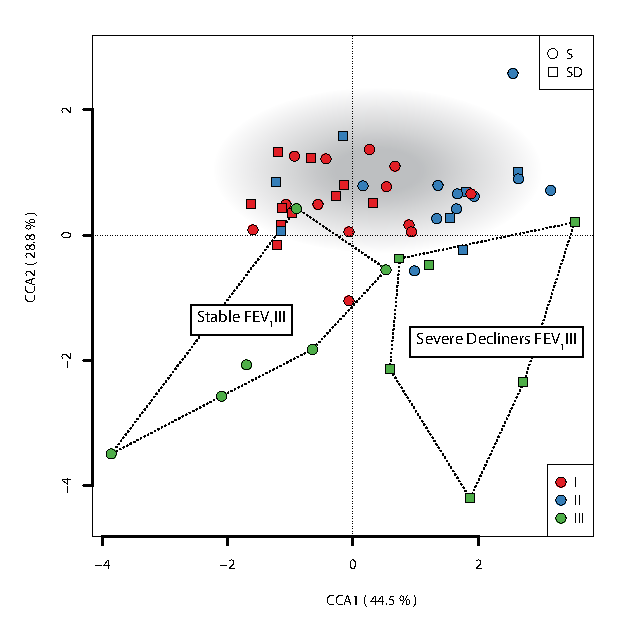
\includegraphics[width=0.7\textwidth]{./figures/Chapter_7/Figure_4_16s}
  	\caption{\label{fig:fig416s}Results of Canonical Correlation Analysis. The dot colors represent the level of the FEV1 index, whereas the dot shapes correspond to patient condition (S or SD). The grey area shows the section of the plot with the highest level of overlap; on the other hand, two clusters with low level of overlap were reported using a dotted line. These clusters contain all samples from the FEV\textsubscript{1} III group divided according to their condition (S or SD).}
\end{figure}%

\subsubsection{Network analysis}
In order to evaluate the presence of different co-occurrence patterns of OTUs in patients with different status (S and SD), a network of correlations between OTUs was built. This approach has been widely used to successfully explore the interaction between organisms from different environments and to study the association between organisms and their environment \cite{barberan2011using, chaffron2010global}. The networks obtained from the OTU counts of S and SD patients consisted of 44 and 42 OTUs (nodes), respectively (Figure~\ref{fig:fig516s}). The number of links (vertices) of the two networks was 204 and 129, with the SD network containing 75 links less than the S one. Moreover, the S network (Figure~\ref{fig:fig516s} (a)) showed a higher level of interconnections between OTUs with an average degree value of 9.273, against a value of 6.143 of the SD network (Figure~\ref{fig:fig516s} (b)). It is worth of mentioning that bacteria belonging to \textit{Pseudomonas }genus (the blue node in Figure 5) were not linked with any other node in both S and SD. The same approach of network construction was used also to look at potential different patterns in relation to FEV\textsubscript{1} conditions in each status, but no clear differences were observed (Figure SM5).\\%
\begin{figure}[!tb]
	\centering
	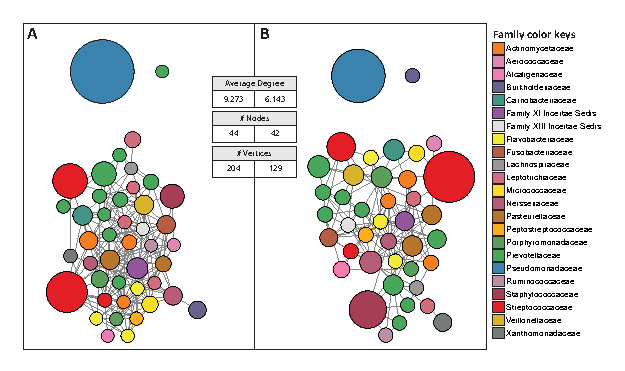
\includegraphics[width=1\textwidth]{./figures/Chapter_7/Figure_5_16s}
  	\caption{\label{fig:fig516s}OTU Networks based on correlation analysis. A connection between two OTUs (nodes) stand for a significant correlation between the two linked OTUs (Spearman's value {\textgreater} 0.6 and p-value {\textless} 0.05). The size of each node is proportional to the OTU count in the dataset. The two panels report the network representation of lung microbiota for both A) Stable and B) Severe decliner patients.}
\end{figure}%

\subsection{Discussion}
During the last 5 years, the perspective of CF airway infection has changed from one based on the analysis of a single pathogen organism to one based on the analysis of the whole lung bacterial community. Several studies have shown that lung bacterial community is very heterogeneous and that this heterogeneity may vary with the age of patients \cite{cox2010airway, rogers2010determining, willner2009metagenomic, rogers2004characterization}. In this study we have inspected the sputum bacterial community of patients with different levels pulmonary functionality, aiming to find a correlation between the exacerbation of the CF disease and the variation in the bacterial community.\\
The 16S rRNA metabarcoding approach used, allowed to sample exhaustively the bacterial diversity (see Figure~\ref{fig:fig316s}) and showed the presence of 22 genera, mainly belonging to both \textit{Proteobacteria} (6 genera) and \textit{Firmicutes} (10 genera) phyla. Interestingly, the phylum showing the highest heterogeneity among S and SD patients and among FEV\textsubscript{1} groups was that of \textit{Proteobacteria, }which in our study was mainly represented by the genera traditionally recognized as CF pathogens (\textit{Haemophilus}, \textit{Pseudomonas}, \textit{Stenotrophomonas}, \textit{Burkholderia}) together with an unclassified genus of the \textit{Alcaligenaceae }family) \cite{lipuma2010changing}. These data allow concluding that indeed culture-based methods provide a good estimation of main taxa which colonize the lung of CF patients. However, since 16S rRNA metabarcoding does not allow defining species or strain identity, we cannot exclude the presence of new species, within those genera, as new opportunistic pathogens of CF patients.\\
Intriguing data were obtained from the analysis of bacterial community diversity and the influence of OTU distribution with respect to the conditions of the patients. Here, OTU distribution and OTU co-occurrence were clearly different between S and SD group. Moreover, when considering the FEV\textsubscript{1} conditions, most of the differences concerned FEV\textsubscript{1} I vs. FEV\textsubscript{1} II groups, for both S and SD patients (Richness) or for S patients only (both Shannon and Evenness indices).\\
Summarizing, our findings allow proposing a scheme of lung bacterial colonization patterns in relation to status (S and SD) and FEV\textsubscript{1} condition (Figure~\ref{fig:fig616s}). Stable patients showed a drop of lung microbiota biodiversity passing from group I to group II of FEV\textsubscript{1} index; we can speculate that between FEV textsubscript{1} I and FEV\textsubscript{1} II something (still unknown) is occurring in the ecology of lung bacterial communities, which may ultimately unbalance bacterial community ecology, opening the way to a more severe condition.\\%
\begin{figure}[!tb]
	\centering
	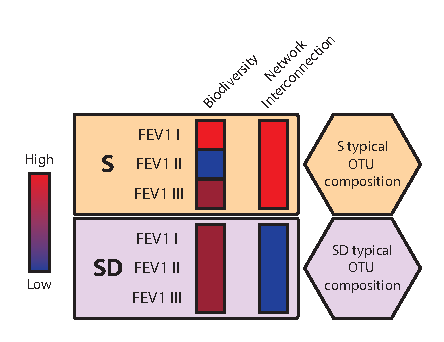
\includegraphics[width=0.6\textwidth]{./figures/Chapter_7/Figure_6_16s}
  	\caption{\label{fig:fig616s}Model of lung bacteria colonization. Two distinct patterns are reported for both S and SD patients showing diverging characteristics.}
\end{figure}%
We can speculate, in an ecological perspective \cite{conrad2013cystic}, that a relatively complex bacterial community is present only in patients with a low level of disease (first group of FEV\textsubscript{1}), whereas, higher levels of pulmonary deficiency (in patients not under exacerbation, the S group), can lead to a drastic decrement of the lung bacterial community complexity leaving the way clear for the proliferation of pathogens bacteria (prevalence of diversity in members of  \textit{Proteobacteria} phylum).\\
As a consequence, we can advocate that bacterial lung microbiota is modified along with changes in CF patient conditions. In particular, as highlighted by network analysis, S patients have a more complex and interconnected lung microbiota than the SD ones. We can then hypothesize that the reduction of bacterial community connections may be due to a higher level of lung colonization from pathogenic bacteria (again the prevalence of members of \textit{Proteobacteria} phylum). This, in turn, may lead to a selection of opportunistic taxa with a lower positive correlation with the others. Here, the absence of correlation of \textit{Pseudomonas} representatives with the other detected OTUs could reinforce the role that members of this genus (e.g. \textit{P. aeruginosa}) may have in pulmonary damage.\\

%%-----------
%% Backmatter
%%-----------
\backmatter
\chaptermark{Bibliography}
\renewcommand{\sectionmark}[1]{\markright{#1}}
\bibliographystyle{unsrt}                           %Use alpha codes for references
\sectionmark{Bibliography}
\addcontentsline{toc}{chapter}{Bibliography}        %Force addition of Bibliography to TOC    
\bibliography{References}

\stopthumb
\mainmatter
\part{Conclusions}
\newthumb
%%%%%%%%%%%%%%%%%%%%%%%%%%%%%%%%%%%%%%%%%%%%%%
\logvartrue
\chapter{General Conclusion and Future Perspectives}
%%%%%%%%%%%%%%%%%%%%%%%%%%%%%%%%%%%%%%%%%%%%%%
The inclusion of the suffix ``meta'' in the word genomic is a tale of two different fields of microbiology which share a common background: clinical microbiology and environmental microbiology. With the development of the small subunit RNA phylotype technique and its application to environmental data, microbiologists have been able to explore bacterial communities in different environments making inference on the dynamics between bacterial cells sharing the same habitat. In addition, several research efforts have been focused on characterizing microbial populations by obtaining estimates of the number and the taxonomy of individuals within the inspected community. Temporal changes in a population are able to inform us about the growth rate of that population, whereas geographic or spatial changes tell us about the existing connections between the environment and the bacterial species living in it. The analysis of this ``universally conserved'' gene has transformed microbial ecology from a primarily descriptive discipline to a fully-fledged quantitative ecology discipline. On the other hand, the metagenomic approach has allowed clinical microbiologists to overcome the limitations imposed by the standard microbiological methods based on the isolation and the successive cultivation of microorganisms. Therefore, the ``meta'' approach has let to the detection of novel bacterial strains able to cause infection diseases or to worsen patients conditions. The assembly of whole bacterial genomes directly from patient samples has provided the high-resolution details necessary to understanding the genetic basis of bacterial pathogenesis, its evolutionary foundations, and the development of new therapeutic treatments for disease. Despite these conceptual changes in microbiology, it is worth noticing that the application of metagenomic approaches has been fuelled by substantial technological advancements in DNA sequencing and analysis of produced data. But all these technological and conceptual advances have introduced new problems related to the analysis of metagenomic data. Indeed, the increasing number of sequences generated from metagenomic studies is often difficult to handle using the existing tools, not specifically designed for this purpose (e.g. the available database searching algorithms are very slow if used for metagenomic data). In addition, analysing complex bacterial communities remains a challenge because of both experimental and data analysis problems. The development of methods and software explicitly designed to cope with all the problems related to metagenomic studies is becoming mandatory for making a step forward in this novel discipline. In this perspective, the interest in bioinformatics as a separate field of science is increasing every year. Therefore, bioinformatics is becoming an interdisciplinary field aiming at the development of methods and software tools for understanding biological data. This discipline combines computer science, statistics, mathematics, and engineering to study and process data obtained from biological experiments. Developing bioinformatic software that can be easily used even by wet-lab microbiologists will be an inevitable stage in the metagenomic perspective. Providing bioinformatic tools either with web-interfaces or with graphical user interfaces will help the diffusion of these instruments making possible for microbiologists to analyse their own data without the need to know a programming language. In conclusion, in the last decade metagenomics has become a very important field of microbiology both from an environmental and from a clinical point of view. Despite its youth, several efforts have been already taken to develop methods and instruments specifically designed for this discipline. However, from a bioinformatic context metagenomics studies are still difficult to handle resulting in complex and less standardized pipelines. In the future, we must focus our attention on the fine tuning of these methods making this novel field of biology accessible to everyone.\\
									% Conclusions									

\stopthumb
\mainmatter
\part{Appendices}
\appendix
\newthumb
\logvartrue
\chapter{Appendix 1}

\section[Evolution of intra-specific regulatory networks in a multipartite bacterial genome]{Evolution of intra-specific regulatory networks in a multipartite bacterial genome%
\sectionmark{Evolution of intra-specific regulatory networks}}
\sectionmark{Evolution of intra-specific regulatory networks}

The gene regulatory network is an important step in the understanding of how organisms precisely control the expression of gene products and therefore phenotypes. Recent studies have pointed out the importance of regulatory networks plasticity in bacterial adaptation and evolution. The evolution of such networks within and outside the species boundary is still obscure though. \textit{Sinorhizobium meliloti} is an ideal species for such study, having three large replicons, many genomes available and a significant knowledge of its TFs. Each replicon has a specific functional and evolutionary mark which might also emerge from their regulatory signature.\\
Here we study the plasticity of the regulatory network within and outside the \textit{S. meliloti} species, looking for the presence of 41 TFs binding motifs in 51 strains and 5 related rhizobial species. We detected preference of several TFs for one of the replicons, and the function of regulated genes was in accordance with the overall replicon functional signatures: house-keeping functions for the chromosome, metabolism  for the chromid, symbiosis functions for the megaplasmid, thus suggesting a replicon-specific wiring of the regulatory network in the \textit{S. meliloti} species. At the same time a significant part of the predicted regulatory network is shared between the chromosome and the chromid, thus adding an additional layer by which the chromid integrates itself in the core genome.\\
Furthermore, the regulatory network distance was found to be correlated with both promoter regions and dispensable genome evolution inside the species, indicating that both pangenome compartments are involved in the regulatory network evolution. Indeed, genes of the dispensable regulon missing both a TFBS and its cognate TF were shown to likely belong to the dispensable genome, possibly due to the relaxation of selective constraints. Regulatory interactions should then also be considered to predict evolutionary conservation and dynamics in bacterial pangenomes.\\

% Please keep the Author Summary between 150 and 200 words
% Use first person. PLoS ONE authors please skip this step. 
% Author Summary not valid for PLoS ONE submissions.   
\subsection*{Author Summary}
The influence of transcriptional regulatory networks on the evolution of bacterial pangenomes has not yet been elucidated, even though the role of transcriptional regulation is widely recognized. Using the model symbiont \textit{Sinorhizobium meliloti} we have predicted the regulatory targets of 41 TFs in 51 strains and 5 other rhizobial species, showing a correlation between regulon diversity and pangenome evolution, through upstream sequence diversity and dispensable genome composition. We have also shown that genes not wired to the regulatory network are more likely to belong to the accessory genome, thus indicating that regulation imposes a selective constraint on bacterial pangenomes evolution. We have also highlighted a series of TF that preferentially regulate genes belonging to one of the three replicons of this species, indicating the presence of replicon-specific regulatory modules, with peculiar functional signatures. At the same time the chromid shares a significant part of the regulatory network with the chromosome, indicating an additional way by which this replicon integrates itself in the pangenome.\\

\subsection{Introduction}
Regulation of gene expression is recognized as a key component in the cellular response to the environment. This is especially true in the bacterial world, for two reasons: bacterial cells are often under severe energy constraints, the most important being protein translation \cite{depardieu2007modes} and they usually face a vast range of environmental and physiological conditions; being able to efficiently and readily react to such conditions can most certainly give a selective advantage over competitors.\\
Transcription is mainly regulated by proteins, called transcription factors (TF), which usually contain a protein domain capable of binding specific DNA sequences, called TF binding sites (TFBS). Depending on the position of the TFBS with respect to the start codon of the regulated gene, the transcription factor can act either as an activator or a repressor of transcription, mostly because of its interaction with the RNA polymerase and its sigma factors \cite{gruber2003multiple, van2009mechanisms}. The binding of the TF to its cognate TFBS is based on non-covalent interactions whose strength is indicated by the so-called affinity constant. Since TFBS can have variations around a preferred sequence, the affinity of a TF for its TFBSs covers a continuous range of values; however, since the TF binding strength appears to follow a sigmoid behaviour, it is possible to distinguish between 'weak' and 'strong' TFBSs \cite{lassig2007biophysics}.\\
As opposed to eukaryotic species, prokaryotic TFBS are usually distinguishable from the 'background DNA', and they tend to have a simpler structure and a close proximity to the transcription start site \cite{wunderlich2009different}. The application of information theory concepts to TFBS has highlighted the dependency of the TF binding specificity to the so called information content of its TFBS, which depends on its length, variability and composition with respect to the overall genomic background (i.e. the sequence composition). The minimum information content for a TF motif to be specifically recognizable intuitively depends on the genome size and genome composition: in a large genome the probability of a false positive is larger and much larger if the composition of the TFBS is close to the background DNA composition. Transcription factors with low information content TFBS usually control the transcription along the whole genome, such as alternate sigma factors and also show a larger variability between species \cite{quinn2014bacterial}; the gene targets of these TFs are also harder to reliably predict, for the presence of many putative site along the whole genome. Bacterial TFs are also usually encoded in the proximity of their targets; their orientation with respect to the regulated genes can also be used to infer whether the TF acts with a positive or negative interaction \cite{janga2007internal, westholm2008genome}. The high gene density of bacterial genomes and its organization in operons results in the expression or repression of whole functional pathways in response to stimuli, again highlighting the influence of cellular energy constraints. Furthermore, the presence of several TFBS in the upstream region of a gene can result in a complex transcriptional response that recall logic gates \cite{hunziker2010genetic}.\\
Prediction of TFBSs in a genome usually relies on the availability of a position specific scoring matrix (PSSM) storing the frequency of each nucleotide at each position of known TFBSs. PSSM modeling the variability of a TFBS can be built by identifying enriched DNA patterns in promoter regions of genes that are known to be under the control of the TF under analysis, or through other assays like the binding of the TF to synthetic nucleotides. Several algorithms have been developed to use such PSSM to search for TFBS in nucleotide sequences, such as the MEME suite \cite{bailey2009meme}, RSAT \cite{van2003regulatory, thomas2008rsat, thomas2011rsat} and the Bio.motif package \cite{cock2009biopython}; a recent alternative method relies on the construction of a hidden markov model (HMM) from an alignment of nucleotide sequences, which can then be searched inside a query nucleotide sequence \cite{eddy2009new, johnson2010hidden, eddy2011accelerated}. Since all these methods and their different implementations have different weaknesses, it has been advised to use a combination of those methods in a search of TFBS inside a genome \cite{harbison2004transcriptional}.\\ 
Regulatory networks in bacteria evolve rapidly, making the comparisons between distant organisms difficult \cite{babu2006evolutionary, gelfand2006evolution, janga2007structure, lozada2006bacterial}. At broad phylogenetic distances, it has been shown that the conservation level of a TF is lower than the one of its targets, but also that species with similar lifestyles tend to show conservation of regulatory network motifs, despite significant variability in the gene composition of the network, suggesting an evolutionary pressure towards the emergence of certain regulatory logics \cite{babu2006evolutionary}.\\
The fluidity of most transcriptional regulatory connections is well known and documented not only at large phylogenetic distances, but at the level of intra-species comparisons too \cite{hendriksen2007regulation, brilli2010diversity, frandi2010comparative, galardini2011exploring}. 
Experiments have shown that Bacteria have high tolerance towards rewiring of regulatory circuitry and, then, they can possibly exploit radical changes in regulatory targets, without extensive changes in phenotypes \cite{isalan2008evolvability}. At the same time, examples where a single change in the regulatory network results in a change in phenotype have been reported \cite{somvanshi2012single, blount2012genomic}. Consequently, there is a large evolutionary potential in bacteria provided by the plasticity of both the genome and its regulatory circuitry. The extent of variability and evolution of the regulatory network inside a species is however still poorly understood.\\
The aim of this study is to apply a comparative genomics approach to regulatory network predictions, deciphering the impact of the regulatory network variability on pangenome evolution. We decided to use the \textit{Sinorhizobium meliloti} species, the nitrogen-fixing symbiont of \textit{Medicago} plants, for which an extensive knowledge on TF is present in the literature \cite{krol2011rhizoregnet, schluter2013global}. This species presents a marked genomic difference with respect to well-know model species, as \textit{Escherichia coli}, since the genome comprises three main replicons of comparable size: a chromosome, a chromid \cite{harrison2010introducing} and a megaplasmid, each one with distinct functional and evolutionary signatures \cite{galibert2001composite, galardini2013replicon}, raising the question if the evolution of the regulatory network may be influenced by functional and evolutionary differences among replicons. Recent reports have shown that there are only two genes essential for growth in minimal media and soil encoded in the \textit{S. meliloti} chromid\cite{maclean2014examination}, even though the chromid harbours many core genes. Moreover, \textit{S. meliloti} has several genomes sequenced to date \cite{galibert2001composite, galardini2011exploring, schneiker2011complete, li2012draft, sugawara2013comparative, weidner2013genome, martinez2013complete, sallet2013next, Galardini2013sigs} and the potential for biotechnological and agricultural applications, which could benefit from the insights generated from a regulatory network analysis. At the gene level, the pangenome of this species has a significantly large fraction of conserved genes of around 5000 gene families \cite{galardini2013replicon, sugawara2013comparative}.\\
We have therefore constructed the comparative regulatory network of the \textit{S. meliloti} species, using the PSSM of 41 TFs collected from the literature and public databases and applying a combination of TFBS prediction methods, combining this predictions with the information about core and dispensable gene families. We have also predicted the presence of the same TFBS to other five closely related rhizobial species (termed 'outgroups': \textit{Rhizobium leguminosarum} bv. \textit{viciae}, \textit{Rhizobium etli}, \textit{Mesorhizobium loti}, \textit{Sinorhizobium fredii} and \textit{Sinorhizobium medicae}), in order to highlight the different behaviours that are present within and between species. Our predictions and other comparative genomics observations are publicly available \href{https://github.com/combogenomics/rhizoreg/tree/paper}{here}.\\

% Results and Discussion can be combined.
\subsection{Results}

\subsubsection{General features of the predicted regulatory network of \textit{S. meliloti}}
As the variable component of the \textit{Sinorhizobium meliloti} pangenome accounts for about 40\% of their proteome size \cite{galardini2013replicon, sugawara2013comparative}, it is reasonable that the same proportion could be also applied to transcription factors (TFs).\\
Based on COG annotations, all the 51 S. meliloti  strains analysed in this study, have been found to encode a similar number of predicted TFs (552 average); a similar number has been also found in the five outgroups (average 533).\\
This is in accordance with previous reports correlating genome size with the number of TFs \cite{charoensawan2010genomic}; alpha-rhizobial genomes, which are known to have larger genomes compared to other bacteria from the same phylum \cite{pini2011plant}, have then the largest collection of TFs in the known bacterial kingdom.\\
About 70\% of all the TFs encoded in the \textit{S. meliloti} pangenome belong to the core genome, while the remaining TFs appear to be singletons in the pangenome, belonging to just one strain or very few (2-3 strains); this orthologous genes distribution is similar to the one observed for the whole pangenome \cite{lobkovsky2013gene} (Figure SM1).\\
 Given the relatively high conservation of TFs in the \textit{S. meliloti} pangenome, most of the 41 TFs analysed in this study were found to be conserved in all strains, the only notable exception being RhrA, the activator of the rhizobactin regulon, which has been found to be absent in 18 strains (35\% of the total). This confirms earlier reports on the variability in presence of this system related to symbiosis \cite{lynch2001genetic, gill1991high, galardini2011exploring}. More interestingly, recent reports have demonstrated how the presence of the rhizobactin operon confers competitive advantage over other \textit{S. meliloti} strains in iron limited environments \cite{maclean2014examination}; we could therefore speculate that a significant fraction of the \textit{S. meliloti} strains have a competitive disadvantage in the absence of iron.\\
 Surprisingly, an ortholog of FixJ (an important symbiosis key regulator) was not predicted in two \textit{S. meliloti} strains (A0643DD and C0438LL), but this could most likely be due to the annotation draft state of these genomes.\\
As expected, more TFs (16) were absent in at least one of the other five outgroups, many of whose orthologs are encoded in the \textit{S. meliloti} symbiotic megaplasmid pSymA (6 TFs out of 9 analysed), including two copies of NodD, FixJ, RctR, SyrM and RhrA (Figure SM1).\\
 Such difference between intraspecific and interspecific TF gene content may anticipate a similar difference at the downstream regulatory network, for the absence of cross-regulatory links.\\
To ensure a high confidence in the TFBS predictions we selected the TF motifs with relatively high information content (see Materials and Methods).\\
We observed a wide range of information gain for TFBSs; of the starting 83 TFBS retrieved from literature and databases, 41 have been found to have enough information content to reliably predict their TFBS (Figure~\ref{fig:reg1} (a), Table SM1).\\%
\begin{figure}[!tb]
	\centering
	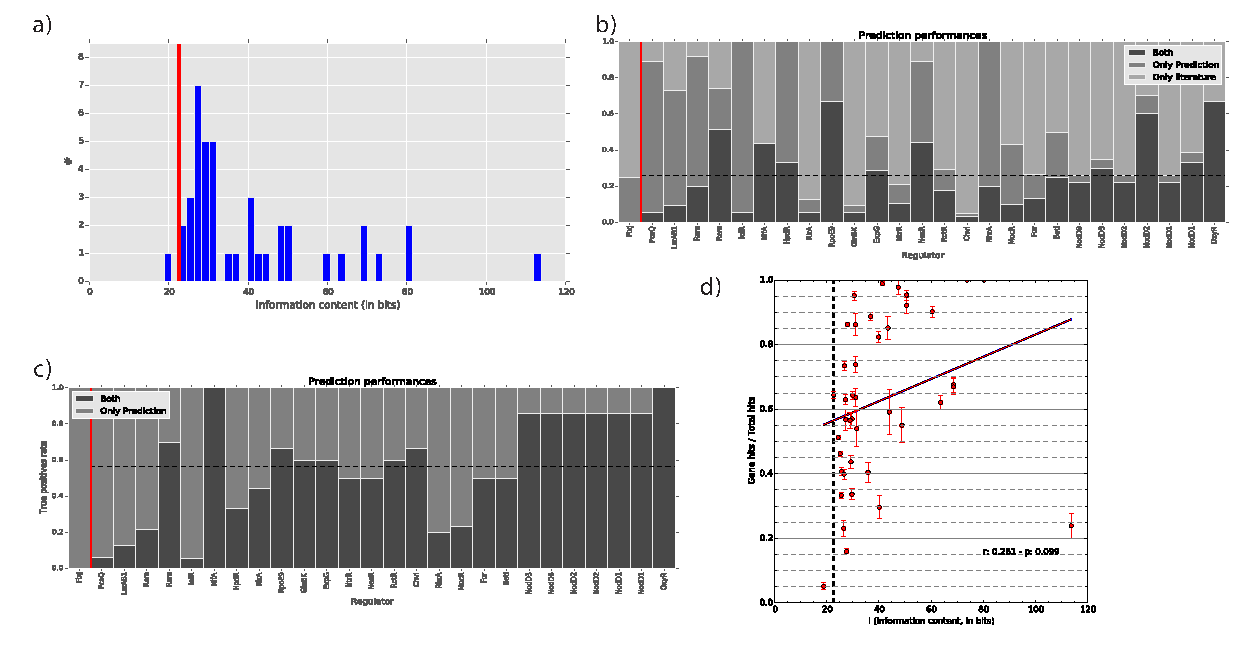
\includegraphics[width=1\textwidth]{./figures/Appendix_1/1_reg}
  	\caption{\label{fig:reg1} General characteristics of the presented TF predictions and quality control. a) Information content frequencies for the 41 analysed TFs: vertical line indicates the minimum information content, as measured for \textit{S. meliloti} strain Rm1021; b-c) comparison between TFBS predictions and the reported experimental results in strain Rm1021: the dashed horizontal line indicates the mean value for the TFs with information content higher than the minimum value; d) correlation between the TFs information content and the signal-to-noise ratio: vertical bars indicate the error level measured in all the strains.}
\end{figure}%
For FixJ two separate motifs acting together have been described \cite{ferrieres2002two}, one above and one slightly below the threshold: both motifs have been used.\\
We applied a novel TFBS prediction approach to overcome common problems associated with the prediction algorithms and maximize accuracy and sensitivity \cite{van2009mechanisms}, including operon predictions to recover most of the downstream regulated genes (see Materials and methods).\\
 The predictions accuracy was determined with a comparison with the downstream regulons reported in the literature, when available (Figure~\ref{fig:reg1} (b and c)); the average accuracy of the predictions was found to be around 55\%, with a tendency to positively correlate with the motif information gain (Figure SM2).\\
On the other hand, a relatively high number of downstream genes were predicted only in the literature.\\
This behaviour may be explained by the fact that most regulons have been defined on the basis of gene expression data; since these experiments are not focused on genes directly under the control of a specific TF, many targets can be regulated by TFs which are downstream in the regulatory cascade and therefore cannot be predicted by our search strategy.\\
Predicted TFBS in genes upstream regions against TFBS predicted in coding regions were considered a signal to noise ratio (upstream hits on total hits) to measure the predictions quality (Figure~\ref{fig:reg1} (d)); for more than 70\% of the analysed TF the observed ratio was above 50\%, with a very poor correlation with the motif information content.\\
Taken together these results show that our predictions are of fairly good quality. We further experimentally confirmed some of the predictions on a subset of predicted promoters of the NodD regulon (Table SM2).\\%
\begin{figure}[!tb]
	\centering
	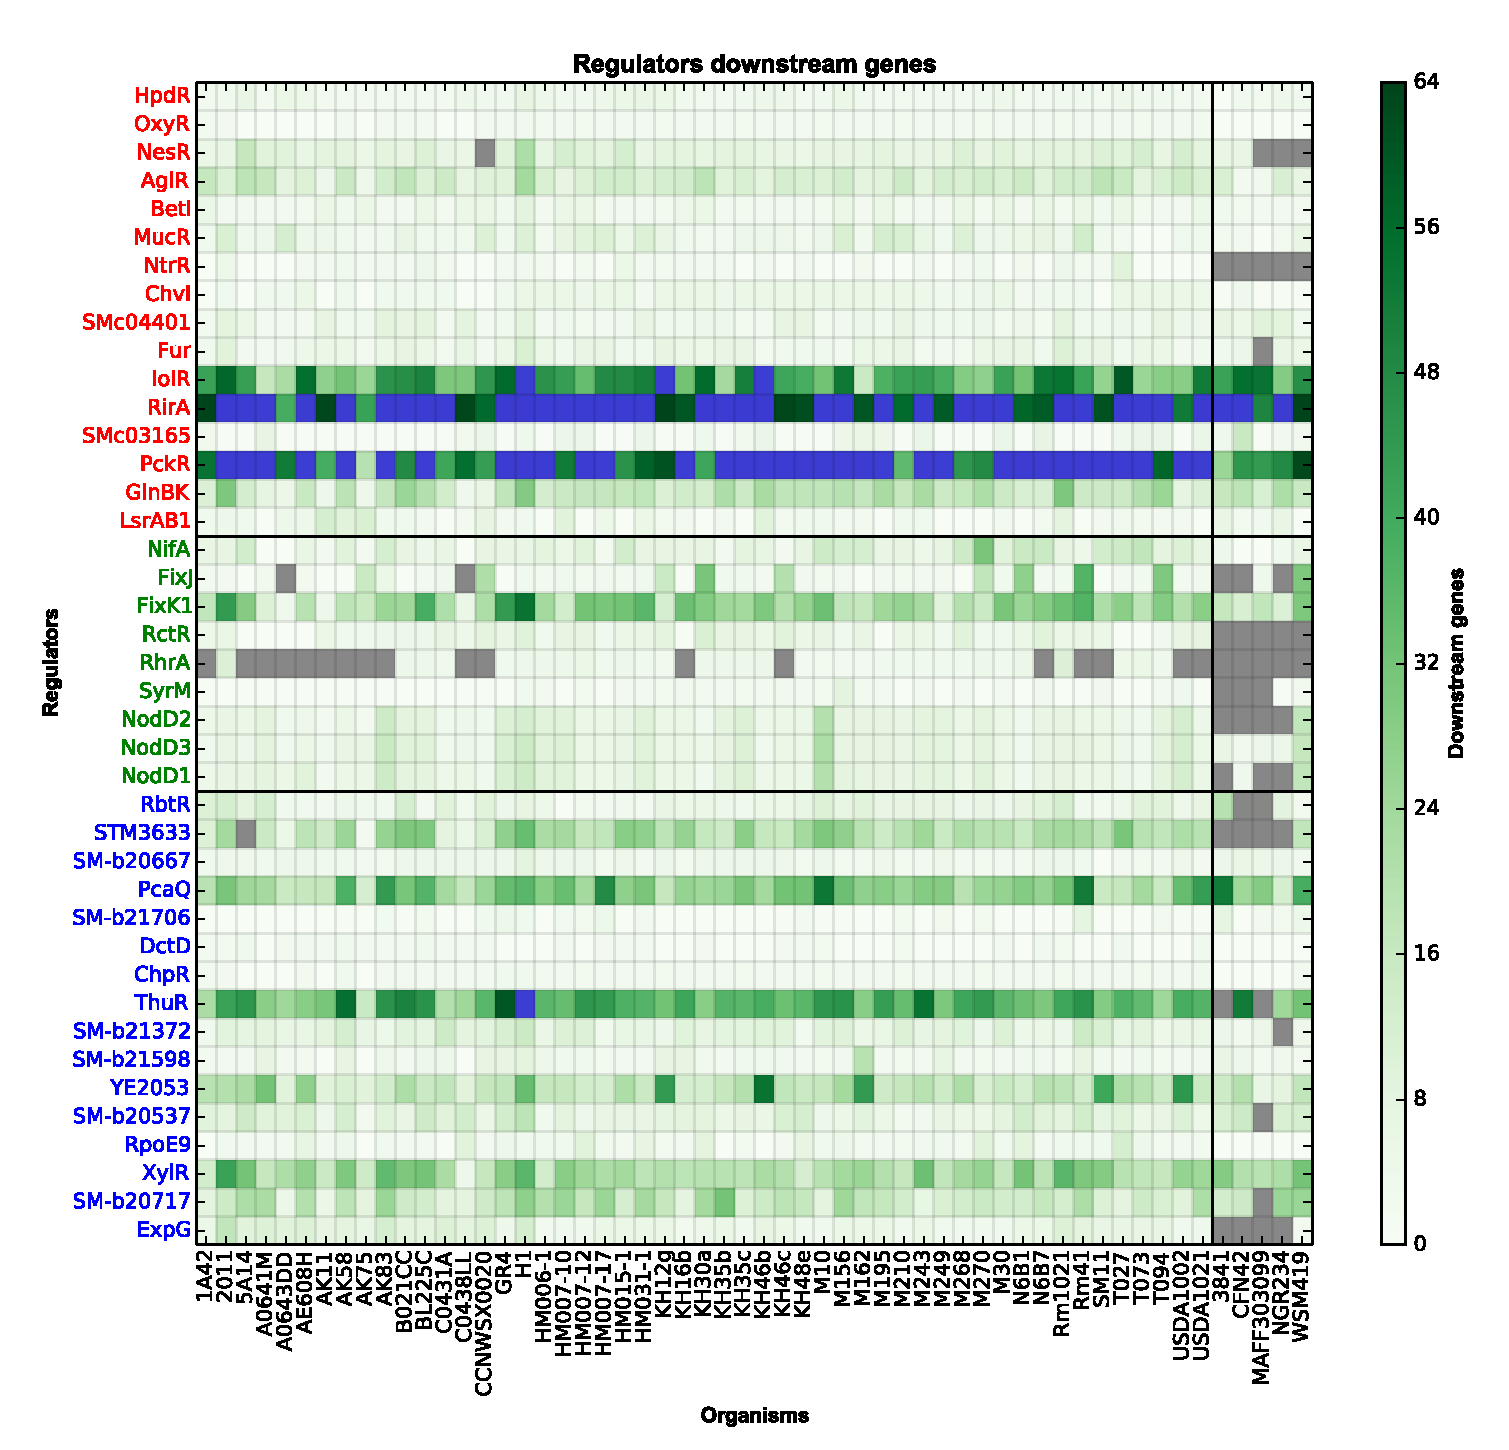
\includegraphics[width=0.7\textwidth]{./figures/Appendix_1/2_reg}
  	\caption{\label{fig:reg2} Variability in regulon size. Color intensity indicates the number of downstream regulated genes in each strain; gray squares indicate the TF absence in the genome of that particular strain. Blue squares indicate that there are more than 64 genes predicted to be under the control of the TF. TFs are colored according to the replicon they belong to: red for chromosome, green for the pSymA megaplasmid and blue for the pSymB chromid}
\end{figure}%
Little variability in the number of genes under the control of each TF was observed between the \textit{S. meliloti} strains (Figure~\ref{fig:reg2} and Table \ref{tab:regulonstats}).\\
Each TF was predicted to control the transcription of about 12 genes in average, with RirA showing the largest regulon (71.6 genes average) and SyrM the smallest one, controlling the transcription of a single gene (1.1 average).\\
\begin{table}[!ht]
\centering
\tiny
\begin{tabular}{ c c c c c c c c c c }
\hline
    ~ & ~ & \multicolumn{2}{ c }{\textit{S. meliloti}} & \multicolumn{2}{ c }{Outgroups} \\
    Regulator & $Replicon^{a}$ & Mean regulon size           & $MAD^{b}$  & Mean regulon size          & $MAD^{b}$  \\
    \hline\hline
    HpdR       & Chromosome        & 3.10  & 1.0  & 2.4           & 1.0  \\
    OxyR       & Chromosome        & 1.71  & 0.0  & 0.0           & 0.0  \\
    NesR       & Chromosome        & 8.24           & 1.0  & 6.0           & NA  \\
    AglR       & Chromosome        & 11.69  & 2.0   & 6.4           & 4.0 \\
    BetI       & Chromosome        & 3.22  & 0.0  & 2.2           & 0.0  \\
    MucR       & Chromosome        & 5.20  & 1.0  & 2.4           & 0.0  \\
    NtrR       & Chromosome        & 1.57  & 2.0  & NA           & NA  \\
    ChvI       & Chromosome        & 3.53  & 1.0  & 0.6           & 0.0  \\
    SMc04401   & Chromosome        & 4.04  & 1.0  & 6.4           & 9.0  \\
    Fur        & Chromosome        & 4.45  & 2.0  & 4.5           & 1.0  \\
    IolR       & Chromosome        & 41.80  & 10.0 & 45.4          & 7.0 \\
    RirA       & Chromosome        & 71.55  & 8.0  & 78.2          & 4.0 \\
    SMc03165   & Chromosome        & 1.69   & 0.0  & 4.4           & 1.0 \\
    PckR       & Chromosome        & 69.80  & 13.0 & 45.0          & 3.0 \\
    GlnBK      & Chromosome        & 15.35  & 4.0  & 16.2          & 2.0 \\
    LsrAB1     & Chromosome        & 2.86  & 2.0 & 3.4           & 3.0  \\
    NifA       & pSymA        & 8.02  & 2.0  & 2.6           & 3.0  \\
    FixJ       & pSymA        & 5.86  & 1.0  & 16.5          & NA \\
    FixK1      & pSymA        & 24.27  & 6.0 & 16.8          & 5.0 \\
    RctR       & pSymA        & 4.59  & 2.0  & NA           & NA  \\
    RhrA       & pSymA        & 3.79  & 1.0  & NA           & NA  \\
    SyrM       & pSymA        & 1.10  & 0.0  & 1.0           & NA  \\
    NodD1      & pSymA        & 6.77  & 2.0  & 10.0          & NA \\
    NodD2      & pSymA        & 6.41  & 2.0  & 17.0          & NA \\
    NodD3      & pSymA        & 6.71  & 2.0  & 6.4           & 2.0 \\
    RbtR       & pSymB        & 5.67  & 2.0  & 9.67 & 17.0 \\
    STM3633    & pSymB        & 19.72          & 4.0  & 17.0          & NA \\
    SM-b20667  & pSymB        & 3.18  & 1.0  & 4.0           & 0.0  \\
    PcaQ       & pSymB        & 27.82  & 5.0  & 31.2          & 10.0 \\
    SM-b21706  & pSymB        & 0.80 & 0.0  & 3.0           & 2.0  \\
    DctD       & pSymB        & 1.24  & 1.0  & 0.0           & 0.0  \\
    ChpR       & pSymB        & 1.88  & 0.0  & 0.4           & 0.0  \\
    ThuR       & pSymB        & 37.63  & 7.0  & 36.0          & 28.0 \\
    SM-b21372  & pSymB        & 7.33  & 2.0  & 3.5           & 0.0  \\
    SM-b21598  & pSymB        & 3.51  & 1.0  & 3.4           & 1.0  \\
    YE2053     & pSymB        & 19.47  & 4.0 & 13.0          & 6.0 \\
    RpoE9      & pSymB        & 3.35  & 1.0 & 0.0           & 0.0  \\
    XylR       & pSymB        & 22.61  & 5.0 & 24.2          & 2.0 \\
    SM-b20717  & pSymB        & 15.24  & 4.0 & 19.25         & 11.0 \\
    SM-b20537  & pSymB        & 7.77  & 3.0 & 12.0          & 1.0 \\
    ExpG       & pSymB        & 6.0            & 2.0 & 2.0           & NA  \\
\hline
\end{tabular}
\caption{\label{tab:regulonstats} Regulatory network general statistics over the strains used in this study. $^{a}$ Position according to the Rm1021 reference strain; $^{b}$ Mean Absolute Deviation; NA: not defined}
\end{table}
TFs with lower information gain showed a tendency to control a larger number of genes (Figure SM2), which confirms the influence of the information content on motif recognition.\\
The regulons were found to have similar size in the outgroups; therefore the regulon is at least conserved in size between different species; this could be the result of the conservation of the upstream sequences across the species.\\
However, given the high plasticity in gene content for bacterial genomes, this hypothesis seems less likely; energy constraints on transcription/translation would appear to be a more realistic explanation. We then expected the composition of the regulon to vary across and between the species.\\
Besides similar regulon sizes, we found that an average 40\% of genes belonging to a regulon belong to the accessory genome (Table \ref{tab:regulonconservation}); this implies that although variable, each TF recruits a similar number of genes under its control, at least in the species analysed here.\\
The mechanisms that can explain this phenomenon should therefore be related with both the variability in upstream regions of conserved genes and in the genes whose presence varies across and between the species.\\

\begin{table}[!ht]
\centering
\tiny
\begin{tabular}{ c c c c }
\hline
Regulator & Replicon & \textit{S. meliloti} & \emph{Outgroups}$^{a}$ \\
\hline\hline
HpdR      & Chromosome         & 0.56        & 0.95          \\
OxyR      & Chromosome         & 1.00        & 1.00          \\
NesR      &  Chromosome        & 0.57        & 0.52          \\
AglR      & Chromosome         & 0.57        & 0.48          \\
BetI      & Chromosome         & 0.33        & 0.50          \\
MucR      & Chromosome         & 0.89        & 0.71          \\
NtrR      & Chromosome         & 0.56        & NA              \\
ChvI      &  Chromosome        & 0.98        & 0.86          \\
SMc04401  & Chromosome         & 0.56        & 0.74          \\
Fur       & Chromosome         & 0.49        & 0.73          \\
IolR      & Chromosome         & 0.59        & 0.52          \\
RirA      & Chromosome         & 0.58        & 0.56          \\
SMc03165  & Chromosome         & 0.68        & 0.65          \\
PckR      & Chromosome         & 0.60        & 0.56          \\
GlnBK     & Chromosome         & 0.58        & 0.63          \\
LsrAB1    & Chromosome         & 0.56        & 0.71          \\
NifA      & pSymA         & 0.57        & 0.74          \\
FixJ      & pSymA         & 0.56        & 0.63          \\
FixK1     & pSymA         & 0.56        & 0.63          \\
RctR      & pSymA         & 0.57        & NA              \\
RhrA      & pSymA         & 0.56        & NA              \\
SyrM      & pSymA         & 0.57        & 0.00          \\
NodD1     & pSymA         & 0.56        & 0.65          \\
NodD2     & pSymA         & 0.56        & 0.66          \\
NodD3     & pSymA         & 0.57        & 0.69          \\
RbtR      & pSymB         & 0.57        & 0.46          \\
STM3633   & pSymB         & 0.57        & 0.63          \\
SM-b20667 & pSymB         & 0.57        & 0.53          \\
PcaQ      & pSymB         & 0.57        & 0.51          \\
SM-b21706 & pSymB         & 0.96        & 0.75          \\
DctD      & pSymB         & 1.00        & 1.00          \\
ChpR      & pSymB         & 0.57        & 1.00          \\
ThuR      & pSymB         & 0.58        & 0.47          \\
SM-b21372 & pSymB         & 0.57        & 0.51          \\
SM-b21598 & pSymB         & 0.57        & 0.70          \\
YE2053    & pSymB         & 0.58        & 0.50          \\
RpoE9     & pSymB         & 0.99        & 0.60          \\
XylR      & pSymB         & 0.57        & 0.54          \\
SM-b20717 & pSymB         & 0.56        & 0.52          \\
SM-b20537 & pSymB         & 0.56        & 0.50          \\
ExpG      & pSymB         & 0.56        & 0.45         \\
\hline
\end{tabular}
\caption{\label{tab:regulonconservation} Regulatory network conservation in \textit{S. meliloti} and near rhizobial species. For each regulator the number of conserved downstream genes over the average regulon size is reported. $^{a}$ \textit{S. meliloti} strain Rm1021 is also considered. NA: not defined}
\end{table}

We couldn't predict the regulon of TFs with very low information content.\\
Predictions for low information content TF, showed a very poor accuracy and precision when compared to experimental data found in the literature (data not shown); an efficient search strategy for such TFs using PSSM has still to be developed. However, from an evolutionary point of view, since those TFs are predicted to bind rather “aspecifically” to many sites along the genome, this would result in a large divergence of regulons between strains, as recently reported in comparison among species \cite{quinn2014bacterial}.\\

\subsubsection{Regulatory network evolution at the species level}
To better understand the pattern of variability of the regulatory network within and between species, we have compared it to the divergence among strains based on the pangenome; we expected the regulatory network differences to depend on both divergence in upstream sequences and patterns of genes presence/absence. 

Following the results of the pangenome analysis, the \emph{S. meliloti} and the outgroups pangenomes have been classified into three non-overlapping groups, and for each one a distance matrix between each strain/species has been constructed (see Materials and methods): 1) alignments of core genes, 2) alignments of upstream regions of the core genes, and 3) presence/absence profiles of accessory genes.
 The regulatory network distance has been computed using the metric previously used by Babu and collaborators \cite{babu2006evolutionary}.
 Intuitively, after some point, the divergence in upstream regions should be paralleled by a larger distance in the regulatory network, since the divergence in the sequence will at some point determine a loss/gain of TFBS and therefore have an impact on the structure of the regulatory network.

Similarly, a larger difference in gene content should also be mirrored by a higher variability in the regulatory network, since new genes may be recruited in the network and TFs may be lost/gained.
 On the other hand, we don't expect to observe a strong correlation between coding sequences divergence and changes in the regulon; this is also due to the lower divergence at the coding level between strains, implying that regulon diversity inside a species should be driven by gene content variability and upstream sequences variability. %
\begin{figure}[!tb]
	\centering
	\includegraphics[width=1\textwidth]{./figures/Appendix_1/3_reg}
  	\caption{\label{fig:reg3} Correlations between pangenome diversity and regulatory network distances. R and S indicate the Pearson's and Spearman's correlation coefficients between the regulatory network and each pangenome partition distances. a) correlations inside the \textit{S. meliloti} species; and b) correlation between the outgroups}
\end{figure}%
These hypotheses on patterns of correlations between pangenome evolution and regulatory divergence were confirmed only at the species level (Figure~\ref{fig:reg3} (a)).
The comparison between \textit{S. meliloti} strains showed that the distance in the regulatory network is correlated with both the distance in upstream regions and with gene content (the accessory genome); as expected, the divergence of coding regions showed no significant correlation with the regulatory network distance (Figure~\ref{fig:reg3} (a)). 
Intriguingly, when considering the outgroup species, all three partitions of the pangenome (core, upstream and accessory) were found to be similarly correlated with the regulatory network distance (Figure~\ref{fig:reg3} (b)).
Since the divergence in coding sequences cannot directly influence transcriptional regulation, we proposed that the most likely explanation of the observed very similar correlations is the overall genome divergence between species, which ultimately is reflected by a higher divergence at the regulatory network level.
This is also confirmed by the high correlation between coding regions, upstream regions and dispensable genome (data not shown).
We then concluded that the regulatory network evolution can be correlated with changes in promoter sequence and in the pangenome composition only at the species level, at least in \textit{S. meliloti}.

\subsubsection{Evolutionary dynamics of regulatory networks at different phylogenetic distances}
The dynamics of the evolution of the regulatory network showed remarkable differences between the intra- and inter-specific levels.
Each observed regulatory interaction in the two datasets (\textit{S. meliloti} and the outgroups) and its state across all strains was used to build a hidden markov model (HMM) to infer the preferred state transitions in our predictions (see Materials and methods), that corresponds to the ways the gene regulatory network can grow and shrink.
The possible states of a target gene depend on the presence of the TF, the target gene itself and the upstream TFBS. %
\begin{figure}[!tb]
	\centering
	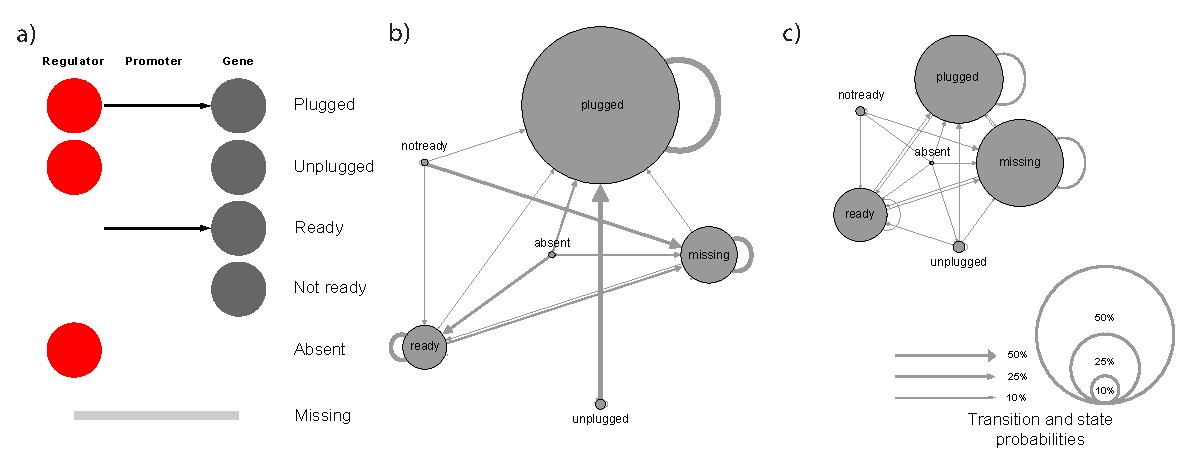
\includegraphics[width=0.8\textwidth]{./figures/Appendix_1/4_reg}
  	\caption{\label{fig:reg4} Regulatory network dynamics. a) Graphical representation of the six states in which each regulatory link (a gene found with a TFBS in at least one genome) can be found in the \textit{S. meliloti} species and between the outgroup species; b) states probabilities and states transitions probabilities inside the \textit{S. meliloti} species: nodes and edges sizes are proportional to the probability in the model; c) states probabilities and states transitions probabilities between the outgroup species}
\end{figure}%
 Then, each target gene can be found in one of six different states (Figure~\ref{fig:reg4} (a): the "plugged" state, the only functional one, which corresponds to a target gene with a TFBS in its promoter region and the TF present in the genome, and other five non-functional states.
 These states miss: i) the TFBS ("unplugged"), ii) the TF ("ready"), iii) both the TF and the TFBS ("not ready"), iv) the regulated gene ("absent") or v) both the TF and the gene itself ("missing").
This HMM can be used to estimate the probability for state transitions, that is the probability of observing a change from one state to another in time.
 Therefore, by looking at the transition probabilities modelled on our predicted regulatory networks we could get an insight on the evolutionary dynamics of the regulatory network, specifically how the gene regulatory network changes in evolution by adding or removing genes.

According to the model, the most represented state in the \textit{S. meliloti} regulatory network is the "plugged" one, indicating conservation of regulatory interactions at the species level (Figure~\ref{fig:reg4} (b) and Table SM3).
More interestingly, the model predicts that the most frequent way through which the regulatory network grows is through the recruitment of "unplugged" genes.
 Very little probability was given to the "plugged" to "missing" transition, indicating that genes belonging to the gene regulatory network are rarely removed from the genome.
 On the other hand, genes with no TFBS and its cognate TF were frequently found to result in the loss of the gene ("not ready" to "missing"), highlighting the importance of regulatory interactions for gene conservation at the species level.
 When considering a wider phylogenetic level (the outgroups), the broader variability in TF gene targets resulted in the "plugged" and "missing" state as equally probable, indicating that regulons might evolve by adding and removing new elements to a conserved kernel of gene targets (Figure~\ref{fig:reg4} (c) and Table SM3).
 This is also reflected in a smaller probability that a target gene i) remains in the "plugged" state when compared to the \textit{S. meliloti} species level, and ii) acquires a TFBS.
 On the other hand, the same probability as inside \textit{S. meliloti} species was observed for the transition "not ready" to "missing", which seems to confirm the importance of regulatory features in explaining the dispensable genome evolution.
 Consequently, a striking different dynamics of regulatory circuitry evolution seems to be present in relation to the taxonomic ranks; at the species level, robust networks are formed and they tend to include new genes from the species pangenome, which then may be fixed if they provide a fitness gain.
On the contrary, when comparing wider taxonomic ranges, regulatory networks are less conserved and apparently genes are included in each species' genome directly with their regulatory features (in a sort of “plug-and-play” model).
% However, we cannot a priori exclude that some of these differences between intra- and inter-species evolutionary behaviour may be overestimated due to the lack of detailed information on the outgroups TFBS.

\subsubsection{Replicon-specific regulation and cross-regulation}
Transcription factors with replicon preference were found to have functional signatures in accordance with the functions encoded in the three main replicons of \textit{S. meliloti}.
 Using a clustering approach on normalized gene hits on each replicon we have found that 19 TFs preferentially regulate genes belonging to one of the three replicons: five to the chromosome (NtrR, OxyR, NesR, ChvI and SMc03165), six to the pSymB chromid (SM-b21706, SM-b20667, ChpR, RbtR, SM-b21598 and SM-b21372) and eight to the symbiotic megaplasmid pSymA (SyrM, NodD3, RhrA, NodD1, NodD2, FixJ, FixK1 and NifA) (Figure~\ref{fig:reg5} (a)); these TFs are also encoded by the same replicon. %
\begin{figure}[!tb]
	\centering
	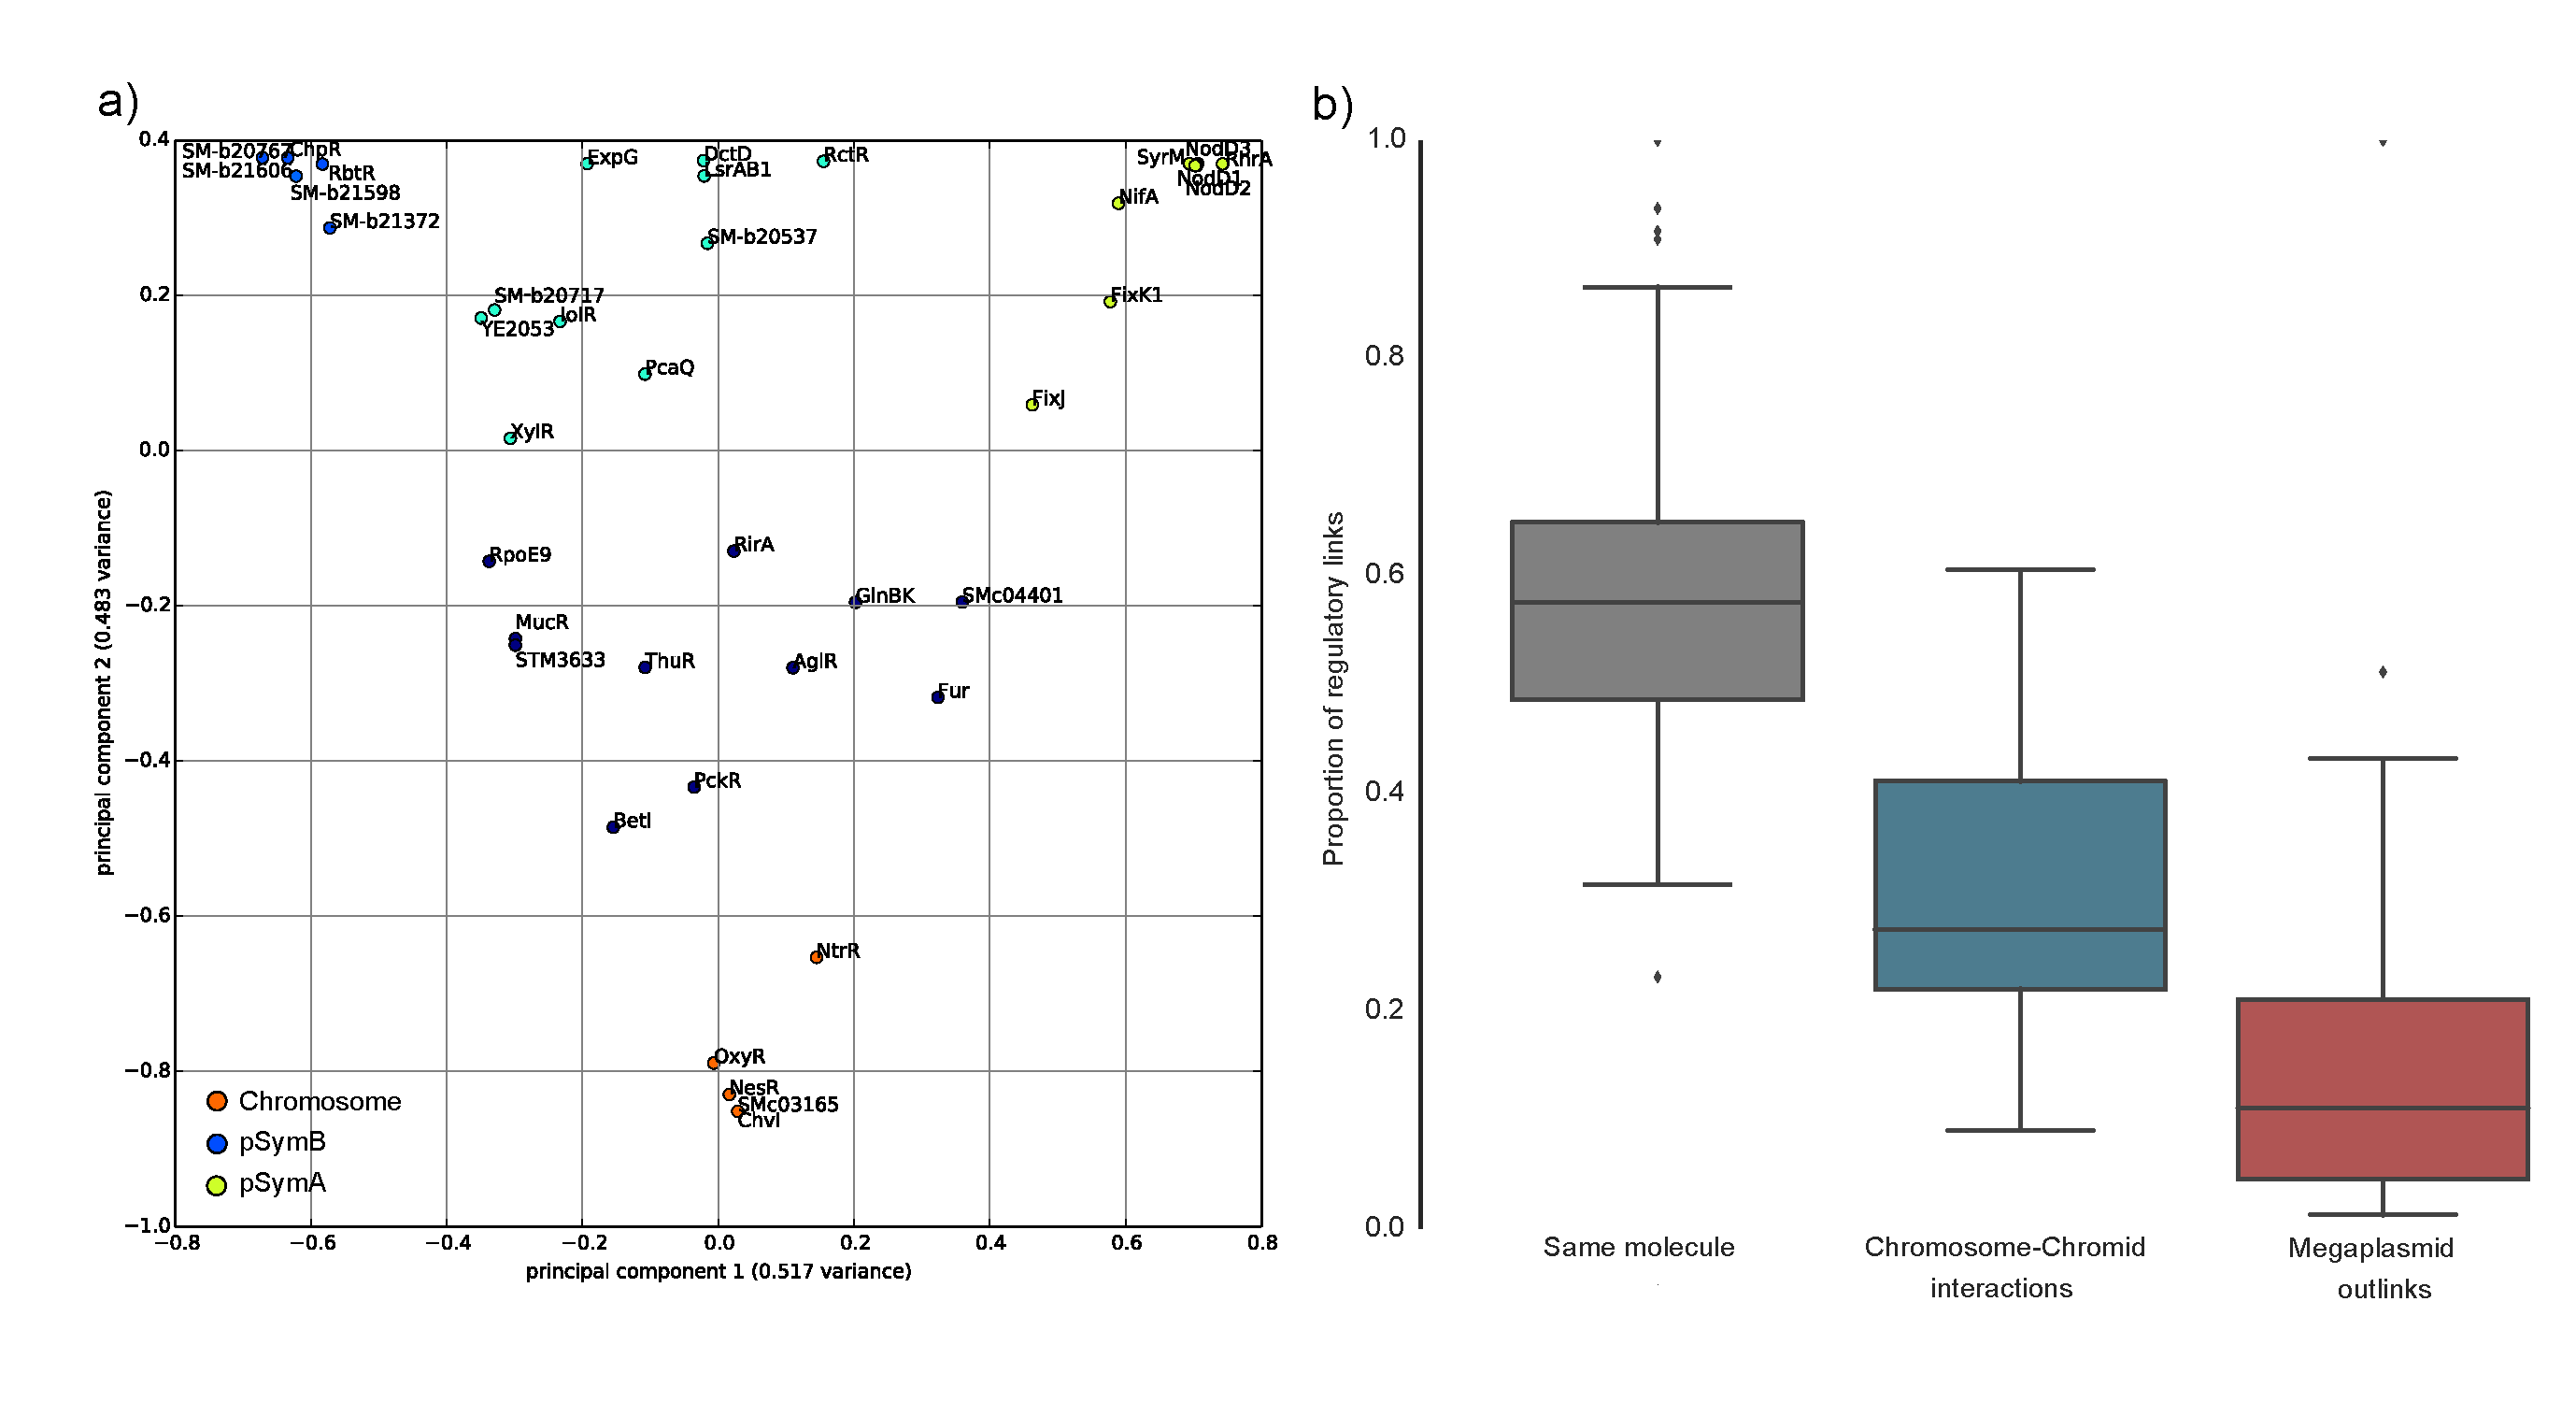
\includegraphics[width=1\textwidth]{./figures/Appendix_1/5_reg}
  	\caption{\label{fig:reg5} TFs preferentially associated with a replicon. a) K-means clustering of the normalized proportion of genes regulated in each replicon of \textit{S. meliloti}, visualized in a two-dimensional PCA; b) Variability in the number of regulatory links in the same replicon and between replicons. All differences are significant (t-test p-value $<$ 0.05)}
\end{figure}%
The six TFs located in the pSymB chromid (whose regulon is also preferentially located on pSymB) appear to mostly regulate the transport and metabolism of various carbon and nitrogen sources, including ribitol (RbtR), tagatose, sorbitol and mannitol (SM-b21372), ribose (SM-b21598), lactose (SM-b21706) and tartrate, succinate, butyrate and pyruvate (SM-b20667).
 The eight TFs present in the symbiotic megaplasmid pSymA (with regulons preferentially located on pSymA) were found to be involved in the regulation of key symbiotic processes, including nitrogenase synthesis and functioning through micro-aerophilia (FixJ, FixK1 and NifA), nod-factors biosynthesis (SyrM, NodD1, NodD2 and NodD3), and iron scavenging (RhrA).

A functional enrichment analysis using COG annotations (Figure SM3) on genes belonging to the regulons of the replicon-biased TFs confirmed this general observation: no functional category was enriched in the chromosome.
 The G category (\emph{carbohydrate metabolism and transport}) was enriched in genes regulated by pSymB encoded TFs, in agreement with the role of chromid pSymB in providing metabolic versatility to \textit{S. meliloti}.
 The C (\emph{energy production and conversion}), U (\emph{intracellular trafficing and secretion}) and T (\emph{Signal Transduction}) categories were enriched in genes under the control of pSymA-harboured TFs, which show some relationship with the establishment on the plant symbiosis.
 This analysis allowed us to depict a scenario where a significant part of the regulatory network is replicon-specific, with a tendency to maintain the functional signature of the host replicon, thus confirming earlier reports on the evolutionary independence of chromids and megaplasmids in \textit{S. meliloti} \cite{harrison2010introducing, galardini2013replicon}.

Interestingly, a fraction of TFs have target genes which span over different replicons, and show a preference for cross regulation between the chromosome and the chromid (Figure~\ref{fig:reg5} (b)).
The presence of cross-replicon regulons, may indeed allow a stabilization of genomic structure, genetically and metabolically connecting chromosome encoded functions with those present in the other two \textit{S. meliloti} replicons.
 In the evolutionary model of the chromid \cite{harrison2010introducing, galardini2013replicon, maclean2014examination}, the stabilization of the chromid into the host genome is related to the acquisition of essential (core) genes in a previously introgressed megaplasmid which gained niche-specific genes.
 Here we found that for TFs encoded on the chromosome (as AglR, GlnBK, IolR, BetI, LsrAB, MucR, PckR, RirA, NesR, RctR) a variable number of target genes are present on pSymB (Supplemental Material S1). The preference for cross-regulation between the chromosome and the chromid, as opposed to the megaplasmid uncovers an additional mechanism by which a chromid integrates itself in bacterial pangenomes.


\subsection{Discussion}

Regulatory networks are key components of cell's response to environmental changes. In the past years, several works have highlighted a high transcriptomic variability, in addition to genomic variation, in strains or individuals from the same species \cite{Cavalieri24102000, kvitek2008variations}.
Consequently, regulatory network variation can have profound impact on local adaptation and fitness of organisms. Recent studies have confirmed that bacterial regulatory networks are able to tolerate the addition of new genes in the transcriptional network \cite{isalan2008evolvability}, which in turn can serve as raw material for selection to operate. Using our original combined search strategy, we indeed found variability in regulon composition within the \textit{S. meliloti} species, which in fact accounted on average on 40\% of the regulon of each strain. On the other hand the regulon size was found to be conserved even outside the species boundary. This could suggest that even though the genes under the control of a TF vary between strains, there is a general constraint on the size of the transcriptional response. Whether this is due to energy constraints or simply an effect due to the genome base composition is yet to be clarified. 

The regulatory network distance (as defined in \cite{babu2006evolutionary}) correlates with upstream regions sequence divergence and patterns of genes presence/absence in the dispensable genome suggest that they both influence the regulatory network composition; the sequence divergence in upstream regions can result in the appearance or disappearance of TFBS, thus changing the regulatory network content. The genes presence/absence patterns in the dispensable genome can also have a strong impact on the regulatory network, with the introduction of new genes with a TFBS. This indicates that the evolution of bacterial regulatory networks, as that of the pangenome can be influenced by mechanisms of gene acquisitions, such as lateral gene transfer, and it's not only linked to gradual mutations in upstream regions.

The evolutionary dynamics of the regulatory network demonstrates the presence of selective pressures that govern gene presence/absence patterns in the dispensable genome. Indeed, even if a significant difference in the state transitions of regulatory links inside and outside the species boundary has been shown,  we have observed a similar tendency to disappear from the pangenome for genes that lack both a TFBS and its cognate TF. This indicates that the dynamics governing pangenome evolution may not be neutral, but also depend on the presence of those genes inside the regulatory network. In fact, fit of theoretical models to the pangenome of several bacterial species has already confirmed that pangenome evolution is under selective pressures \cite{lobkovsky2013gene}; we suggest that regulatory networks have an important role in shaping the bacterial gene content and contribute to genes fitness, which in turn may be linked to environmental adaptation. 

Moreover, the preference of nineteen TFs for target genes on one of the three replicons of \textit{S. meliloti} indicates that in multipartite bacterial genomes, similarly to replicon-dependent patterns of evolution in gene and functions content \cite{galardini2013replicon}, a replicon-specific transcriptional regulation is to be expected. At the same time, a significant number of cross-links between the chromosome and the chromid uncovers an for the first time an additional mechanism by which new replicons integrate into a bacterial pangenome.

% You may title this section "Methods" or "Models". 
% "Models" is not a valid title for PLoS ONE authors. However, PLoS ONE
% authors may use "Analysis" 
\subsection{Materials and Methods \label{sec:mat}}

\subsubsection{Genome sequences}
The 51 genomic sequences belonging to \textit{Sinorhizobium meliloti} and the five genomic sequences from closely related symbiotic species are listed in Table SM4.

\subsubsection{Orthology}
The orthology relationships inside the 51 \textit{S. meliloti} strains has been computed using the Blast-BBH algorithm implemented in the DuctApe suite (version 0.13.0)\cite{galardini2014ductape}, using default parameters. The same analysis has been conducted on the five closely related species with the addition of the Rm1021 reference strain, using the BLOSUM62 scoring matrix to account for their greater sequence diversity.

\subsubsection{Regulators estimation}
The number of regulators present in each genome has been estimated using COG annotations. The similarity of each protein against the COG database has been measured with a rpsblast scan \cite{altschul1990basic}, using an E-value threshold of 1e-10. Each protein mapped to the COG category K (Transcription) has been considered as a putative regulator.

\subsubsection{Regulatory motifs collection}
The 83 regulators whose PSSM has been extracted are listed in Table SM1. For those motifs retrieved from the literature, we collected the upstream regions of the regulated genes and (when available), the consensus binding sites from bibliographical records; the upstream regions have then been analysed with the \textit{meme} program \cite{bailey2009meme}(version 4.9.0), using the model that retrieved the PSMM with higher similarity to literature. Twenty-two motif files have been generated using the information retrieved from the RhizoRegNet database \cite{krol2011rhizoregnet}. Fifteen motif files have been generated using the information retrieved from the RegTransBase database \cite{kazakov2007regtransbase}. For the 5 regulators having more than one predicted motif, for instance those having a variable length (FixJ, RpoD, RpoE2, RpoH1 and RpoH2), one motif file for each motif length has been generated.
All the retrieved motifs have been converted to HMM models using the \textit{hmmbuild} program from the HMMer suite \cite{eddy2009new, johnson2010hidden, eddy2011accelerated}(version 3.1b1), using the alignments present in the MEME motif file.
It has been previously shown that in bacterial genomes TFBS can be reliably distinguished from background DNA only if their information content is higher than the minimum information content for the target genome, which depends on the genome size and composition \cite{wunderlich2009different} (this simplification of course ignores other factors such accessibility or proximity of the RNA polymerase). The information gain of the TFBS with respect to the genome is calculated using the Kullback-Leibler divergence between the corresponding nucleotide frequencies \cite{berg1987selection}, and it has been shown to correlate with the motif length and base composition of the motif with respect to the surrounding genome sequence. TF motifs with sufficient information content also tend to show less variability in their regulon composition between species \cite{quinn2014bacterial}; by focusing our analysis on such TFs we ensured a more precise analysis.
The information content of each motif has been calculated as suggested by Wunderlich et al \cite{wunderlich2009different}, using the Rm1021 reference genome for the calculation of the minimum information content; given the dependence of this variable on genome size and the fact that all the \textit{S. meliloti} strains have similar genome size, there has been no need to calculate a strain specific threshold. Motifs whose information content was found to be lower the minimum information content have been discarded with exception of FixJ, which has two distinct PSSM, one of which is above the threshold. In the presence of more than one source for a regulator (literature, RhizoRegNet or RegTransBase), the motif file having the highest information content has been considered in the final analysis.

\subsubsection{Search of regulatory motifs occurrences}
For each genome, background k-mers frequencies have been calculated using the \textit{fasta-get-markov} program from the MEME suite (version 4.9.0)\cite{bailey2009meme}, using 3 as the maximum value for k.
Each regulatory motif has been searched inside each genomic sequence using four scanning algorithms. The \textit{mast} program from the MEME suite (version 4.9.0)\cite{bailey2009meme} has been used with an E-value threshold of 100 and the use of a genome-specific background file. The \textit{matrix-scan} program from the RSAT suite \cite{van2003regulatory, thomas2008rsat, thomas2011rsat} has been used with a P-value threshold of 0.001, the background file and a pseudocount of 0.01, as suggested by Nishida et al. \cite{nishida2009pseudocounts}. The \textit{Bio.motifs} package from the Biopython library (version 1.62b)\cite{cock2009biopython} has been used with a false negative rate threshold of 0.05 and a pseudocount of 0.01, as suggested by Nishida et al. \cite{nishida2009pseudocounts}. The \textit{nHMMer} program from the HMMer suite (version 3.1b1)\cite{eddy2009new, johnson2010hidden, eddy2011accelerated} has been used with an E-value threshold of 100 and with all the heuristic filters turned off.
Each regulatory motif hit has been parsed, separating the hits being present in the upstream region of a gene from the others. The upstream region has been defined as the intergenic region in front of the first codon with a maximum size of 600 bp. In the case of a palindrome motif, the motif orientation has been ignored.

The distributions of the raw scores has been tested using a normality test, as implemented in the SciPy library (version 0.13.3)\cite{d1971omnibus}\cite{jones2001scipy}. The score threshold has been determined through the calculation of the raw scores quartiles (Q1 and Q3) and defining the score threshold ($\tau_S$ in Eq. \ref{scoreT}) in order to consider only the upper outliers \cite{hojo1931distribution}.

\begin{equation}
\label{scoreT}
\tau_S= Q3 + (1.5 (Q3-Q1)).
\end{equation}


For the Biopython method the bit score has been used, while for the RSAT, HMMer and MEME methods the negative base 10 logarithm of the E-value has been considered. The regulatory motifs predicted by at least three methods have been considered for further analysis. 

\subsubsection{Experimental confirmation of pomoters}
Upstream sequences from selected putative target genes of NodD regulon were analysed (see Table SM2). Sequences (approximately 400 nt upstream the translation start site of the gene) were amplified from crude lisates of \textit{S. meliloti} strains and cloned into pTO2 vector (which carries GFPuv as reporter gene \cite{karunakaran2005family}) by using  \textit{SalI} and  \textit{KnpI} restriction sites. Recombinant clones of \textit{E. coli} S17-1 strain were selected by gentamycin resistance and verified by sequencing of inserted fragments. Positive clones were used for transferring recombinant pOT2 vectors to  \textit{S. meliloti} Rm1021 by bi-parental conjugation by using previously described protocols \cite{pini2014molecular}\cite{pini2013divj}. \textit{S. meliloti} Rm1021 recombinant strains were then tested for GFP fluorescence after incubation of a 5 ml culture grown at the mid-exponential phase with 1 microM luteolin (Sigma-Aldrich) in liquid TY medium at 30$^{\circ}$C for 3h. GFP fluorecence was measured on a Infine200 Pro plate reader (Tecan). Measures were taken in triplicate and normalized to cell growth estimates as absorbance to 600nm.

\subsubsection{Operon prediction}
The operons belonging to the 56 genomes of this study have been predicted using the operon prediction software (version 1.2)\cite{westover2005operon}, using a beta threshold of 0.7 and a probability threshold of 0.5. The number and length of the predicted operons in each strain are listed in Table SM5.

\subsubsection{Replicon mapping}
Each contig of the 44 \textit{S. meliloti} draft genomes has been mapped to the seven complete genomes using CONTIGuator (version 2.7.3)\cite{galardini2011contiguator}, using a 15\% coverage threshold and considering blast hits over 1000 bp in length. A contig has been considered mapped to a replicon When it has been found mapped to the replicon in at least five complete genomes, or when it has been mapped to the replicon in at least one complete genome and to no replicon in the others.

The number of average gene hits have been divided for each replicon (either from a complete genome or a draft genome) and normalized by the number of genes belonging to each replicon in the Rm1021 reference strain. Regulators with preferential regulatory hits in a specific replicon have been highlighted performing a k-means clustering (k=5, selected using an elbow test \cite{ward1963hierarchical}) and plotted using the two principal components of the proportion of hits in each repliconusing the scikits-learn package (version 0.14.1)\cite{pedregosa2011scikit}. Only the three main replicons (chromosome, pSymB and pSymA) have been considered. COG categories enrichment have been tested using a Fisher's exact test, as implemented in the DendroPy package \cite{sukumaran2010dendropy}.

\subsubsection{Phylogenetic distance}
Phylogenetic distance inside the \textit{S. meliloti} pangenome and the pangenome of the five related species has been computed as described in a previous work \cite{galardini2013replicon}. The pangenome has been divided in three fractions, allowing the use of three distinct phylogenetic distances. The "core" distance has been calculated through the alignment of all the nucleotide sequences of each core gene, discarding those genes where at least one sequence was 60bp shorter or longer with respect to the other sequences. The "upstream" distance has been calculated through the alignment of the core genes upstream regions, discarding sequences below 5bp in length. The alignments have been calculated using MUSCLE (version 3.8.31)\cite{edgar2004muscle} and the bayesian tree has been inferred using MrBayes (version 3.2.0)\cite{ronquist2012mrbayes}. The distance matrix for both distance categories has been computed from the phylogenetic tree using the textit{Bio.Phylo} package inside the Biopython library (version 1.62b)\cite{talevich2012bio}. The "accessory" distance has been calculated through the construction of a presence/absence binary matrix for all the dispensable genome OGs; the distance between each strain has been then calculated using the Jaccard distance measure, as implemented in the SciPy library (version 0.13.3)\cite{jones2001scipy}.

\subsubsection{Regulatory network distance}
The distance between each strain inside the \textit{S. meliloti} and the other five related species regulatory network has been computed using the distance in the presence/absence of regulatory interactions as suggested in the work of Babu and collaborators \cite{babu2006evolutionary}. The distance between strain A and B is computed using Eq. \ref{babu}.

\begin{equation}D_{AB} = 1 - \cfrac{core_{AB}}{total_{AB}},
\label{babu}
\end{equation}

where $core_{AB}$ and $total_{AB}$ represent the number of conserved and total regulatory interactions, respectively.

Pearson and Spearman correlation coefficients between the pangenome and the regulatory network distance have been calculated using the implementations of the SciPy library (version 0.13.3)\cite{jones2001scipy}, removing the outliers with mean absolute deviation $>$ 3.5.

\subsubsection{Regulatory network transistions}
The state transitions of the regulatory network has been inferred by encoding them in a hidden markov model. Each one of the regulatory links observed in at least one strain has been tested for their state in each organism, following the labelling of Figure~\ref{fig:reg4} (a). Specifically, each regulatory link in the network of each organism could belong to one of the following categories:

\begin{itemize}
\item \textbf{Plugged:} regulator, gene and TFBS present
\item \textbf{Unplugged:} regulator and gene present, TFBS absent
\item \textbf{Ready:} gene and TFBS present, regulator absent
\item \textbf{Not ready:} gene present, regulator and TFBS absent
\item \textbf{Absent:} regulator present, gene and TFBS absent
\item \textbf{Missing:} regulator, gene and TFBS absent
\end{itemize}

The hidden markov model has been constructed using the Baum-Welch algorithm \cite{jelinek1975design}, as implemented in the GHMM python library. Transitions probability between states has been inferred averaging 1000 HMMs, constructed through a randomization of organisms order. 

\subsubsection{Results analysis and visualization}
Regulatory motifs data has been analysed and visualized using the NumPy \cite{van2011numpy} and matplotlib \cite{hunter2007matplotlib} libraries inside the iPython environment \cite{perez2007ipython}. Regulatory networks have been built using the networkx library \cite{networkx} and visualized using Gephi \cite{bastian2009gephi}.

\subsubsection{Data and methods availability}
Genomic sequences, regulatory motif files and search and analysis scripts are available as separate git repositories. The rhizoreg repository (https://github.com/combogenomics/rhizoreg/tree/paper), contains the input data; the regtools repository (https://github.com/combogenomics/regtools/tree/paper) contains the main scripts used to conduct the analysis.


%%-----------
%% Backmatter
%%-----------
\backmatter
\chaptermark{Bibliography}
\renewcommand{\sectionmark}[1]{\markright{#1}}
\bibliographystyle{unsrt}                           %Use alpha codes for references
\sectionmark{Bibliography}
\addcontentsline{toc}{chapter}{Bibliography}        %Force addition of Bibliography to TOC    
\bibliography{References}                                 %Appendix A
\mainmatter
\newthumb
\logvartrue
\chapter{Abreviations}

\begin{itemize}
\item \textbf{DNA}: Deoxyribonucleic acid
\item \textbf{RNA}: Ribonucleic acid
\item \textbf{rRNA}: Ribosomial RNA
\item \textbf{16S}: Component of the 30S small subunit of prokaryotic ribosomes
\item \textbf{BSC}: Biological species concept
\item \textbf{PhSC}: Phenetic species concept
\item \textbf{ESC}: Evolutionary species concept
\item \textbf{ACE}: Abundance-based coverage estimator
\item \textbf{MRR}: Mark-release-recapture method

\item \textbf{PCR}: Polymerase Chain Reaction
\item \textbf{ORF}: Open Reading Frame
\item \textbf{ASCII}: American Standard Code for Information Interchange
\item \textbf{HMM}: Hidden Markov Model
\item \textbf{RBS}: Ribosome Binding Site
\item \textbf{BLAST}: Basic Local Alignment Search Tool
\item \textbf{KEGG}: Kyoto Encyclopedia of genes and genomes
\item \textbf{GO}: Gene Ontology
\item \textbf{COG}: Cluster of Orthologous groups
\item \textbf{LUCA}: Last Universal Common Ancestor
\item \textbf{HGT}: Horizontal Gene Transfer
\item \textbf{BBH}: Bidirectional Best Hit
\item \textbf{NGS}: Next Generation Sequencing
\item \textbf{Mb}: Megabase
\item \textbf{PCR}: Polymerase Chain Reaction
\item \textbf{dNTP}: Deoxynucleoside Triphosphate
\item \textbf{rRNA}: Ribosomial RNA
\item \textbf{PGPR}: Plant growth-promoting rhizobacteria
\item \textbf{ISR}: Induced systemic resistance
\item \textbf{BNF}: Biological nitrogen fixation
\item \textbf{ATP}: Adenosine triphosphate
\item \textbf{Mb}: Megabase
\item \textbf{CGH}: Comparative genomics hybridization
\item \textbf{API}: Application programming interface
\item \textbf{PM}: Phenotype microarray
\item \textbf{API}: Application programming interface
\item \textbf{AV}: Activity index
\item \textbf{PCA}: Principal component analysis
\end{itemize}									%Appendix B

\end{document}
% % % EOF % % %